
\section*{CHƯƠNG 3. THIẾT KẾ HỆ THỐNG}
\setcounter{section}{3}
\setcounter{subsection}{0} %LƯU Ý MỖI LẦN THÊM CHƯƠNG MỚI CẦN THÊM CÂU NÀY ĐỂ RESET THỨ TỰ CỦA SUBSECTON VỀ 1
\setcounter{table}{0} % LƯU Ý SAU MỖI LẦN GỌI BẢNG HAY HÌNH ẢNH PHẢI THÊM CÂU NÀY ĐỂ RESET THỨ TỰ
\setcounter{figure}{0} %% LƯU Ý SAU MỖI LẦN GỌI BẢNG HAY HÌNH ẢNH PHẢI THÊM CÂU NÀY ĐỂ RESET THỨ TỰ
\addcontentsline{toc}{section}{\numberline{}CHƯƠNG 3. THIẾT KẾ HỆ THỐNG}

Chương này sẽ tập trung mô tả quá trình thiết kế hệ thống, từ cấu trúc tổng thể đến các thành phần chi tiết, dựa trên những phân tích đã thực hiện trong Chương 2.
Mở đầu là xây dựng sơ đồ kiến trúc hệ thống.
Tiếp theo, chương tập trung vào thiết kế giao diện người dùng và các chức năng chính cho app cùng server.
Nội dung chính được thể hiện qua hình ảnh và sơ đồ minh họa, không chỉ mô tả chi tiết luồng hoạt động mà còn làm rõ cách các thành phần trong hệ thống phối hợp, hỗ trợ lẫn nhau.
\subsection{Sơ đồ tổng quan kiến trúc của hệ thống}

\begin{figure}[H]
	\centering
	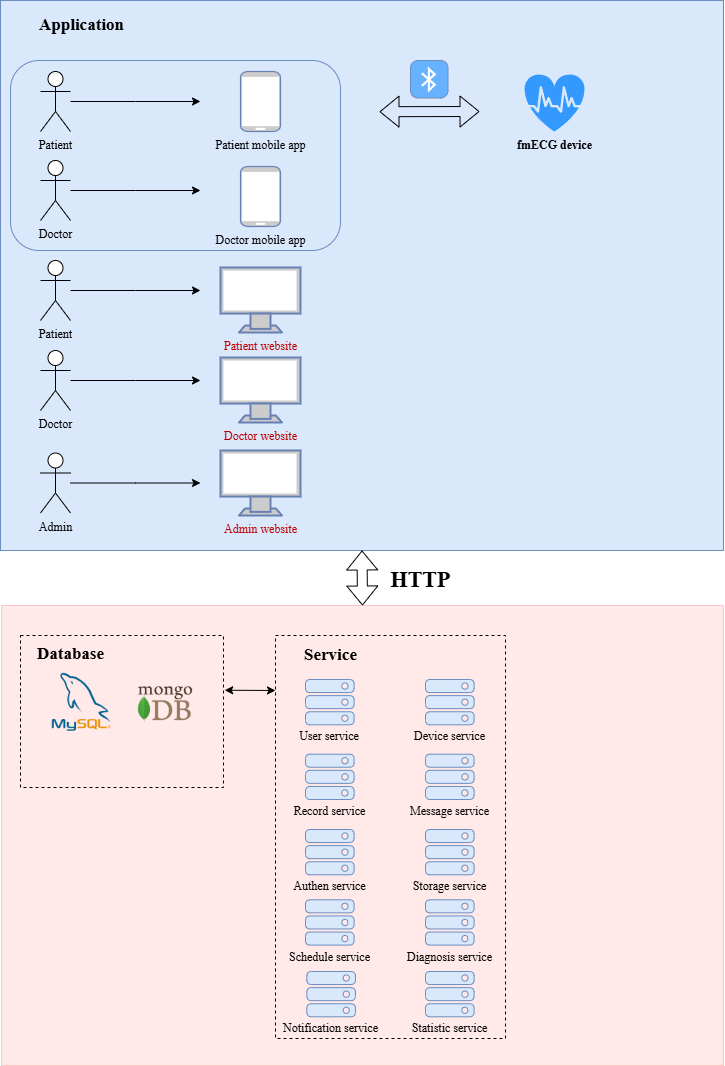
\includegraphics[width=12cm,height=16cm]{Images/System/fmECG_architecture-System_Architecture.drawio.png}
	\caption[Tổng quan kiến trúc hệ thống]{\bfseries \fontsize{12pt}{0pt}\selectfont Tổng quan kiến trúc hệ thống}
	\label{fmECG_architecture-System} %đặt tên cho ảnh
\end{figure}
Hệ thống bao gồm ba thành phần chính: Máy chủ (Server), Thiết bị (Device) và Ứng dụng (Web và App).
Mỗi thành phần đảm nhiệm một vai trò quan trọng, cùng phối hợp để đảm bảo hoạt động của toàn bộ hệ thống như được minh họa trong hình vẽ.

Hình \ref{fmECG_architecture-System} thể hiện ba phần:

\begin{adjustwidth}{1.5em}{}
	\begin{itemize}
		\item Device (Thiết bị): Gồm các thiết bị phần cứng đo các dữ liệu sức khỏe tim mạch, có khả năng kết nối với ứng dụng di động của bệnh nhân thông qua Bluetooth.
		\item Application (Ứng dụng): Bao gồm ứng dụng di động và website, phục vụ nhu cầu sử dụng của bệnh nhân, bác sĩ và quản trị viên.
		\item Server (Máy chủ): Chứa các dịch vụ (Services) xử lý yêu cầu từ ứng dụng và quản lý cơ sở dữ liệu.
	\end{itemize}
\end{adjustwidth}

Trong sơ đồ kiến trúc hệ thống, bệnh nhân sử dụng ứng dụng di động (Mobile App) để kết nối trực tiếp với thiết bị (Device).
Ứng dụng di động thuộc Khối Ứng dụng (Application), chịu trách nhiệm giao tiếp với Khối Máy chủ (Server) thông qua các API và giao thức HTTP.
Khi yêu cầu được nhận từ Application, Server sẽ thực hiện xử lý dữ liệu thông qua các dịch vụ (Services) được thiết kế riêng biệt.
Tùy theo loại yêu cầu, các dịch vụ này sẽ truy xuất hoặc cập nhật dữ liệu trong cơ sở dữ liệu, sau đó gửi kết quả phản hồi cho người dùng,
hoàn thiện quá trình tương tác giữa người dùng và hệ thống.\begin{adjustwidth}{1.5em}{}
	\begin{itemize}
		\item Authen Service: Đảm nhận các nhiệm vụ liên quan đến bảo mật hệ thống, bao gồm mã hóa dữ liệu nhạy cảm, tạo và xác minh token để đảm bảo tính an toàn khi truy cập,
		      quản lý phân quyền người dùng đối với API,và thực hiện mã hóa thông tin trước khi lưu trữ nhằm ngăn chặn rò rỉ dữ liệu.
		\item User Service: Xử lý toàn bộ các thao tác liên quan đến người dùng, như tạo tài khoản mới, xác minh thông tin đăng nhập, lấy thông tin cá nhân của người dùng,
		      đồng thời hỗ trợ cập nhật và chỉnh sửa thông tin cá nhân khi cần thiết.
		\item Device Service: Chịu trách nhiệm quản lý thiết bị, bao gồm các chức năng như thêm mới, chỉnh sửa thông tin, xóa thiết bị,
		      và cập nhật tình trạng thiết bị hoặc thông số liên quan để đảm bảo thiết bị hoạt động đúng trong hệ thống.
		\item Storage Service: Quản lý và vận hành hệ thống lưu trữ dữ liệu, bao gồm lưu trữ file, tài liệu, và các thông tin quan trọng của hệ thống.
		      Đồng thời, đảm bảo tính nhất quán của dữ liệu thông qua cơ chế xử lý race condition, khóa truy cập và đồng bộ hóa dữ liệu trong các trường hợp truy cập đồng thời,
		      cũng như tối ưu hóa hiệu suất lưu trữ và truy xuất dữ liệu.
		\item Record Service: Xử lý các dữ liệu liên quan đến phiên đo, bao gồm thêm mới, cập nhật, xóa dữ liệu, và xử lý các file đo được từ thiết bị trước khi lưu trữ hoặc gửi đến người dùng.
		\item Message Service: Quản lý toàn bộ các yêu cầu liên quan đến nhắn tin, bao gồm gửi, nhận, lưu trữ tin nhắn, hỗ trợ các nhóm trò chuyện giữa những người dùng trong hệ thống.
		\item Schedule Service: Đảm nhiệm việc quản lý lịch khám, bao gồm đặt lịch và xử lý các phản hồi liên quan, nhằm đảm bảo quy trình đặt lịch diễn ra mượt mà giữa bệnh nhân, bác sĩ và hệ thống.
		\item Diagnosis Service: Quản lý các tác vụ liên quan đến chẩn đoán, bao gồm thêm mới và chỉnh sửa thông tin chẩn đoán cho bệnh nhân, đảm bảo dữ liệu chính xác và hỗ trợ quá trình điều trị hiệu quả.
		\item Notification Service: Đảm bảo quản lý hiệu quả các thông báo cho người dùng, từ việc gửi thông báo sự kiện, cảnh báo, đến nhắc nhở,
		      giúp người dùng cập nhật kịp thời các thông tin quan trọng từ hệ thống.
		\item Statistic Service: Chịu trách nhiệm tổng hợp số liệu thống kê trong hệ thống, bao gồm số lượng người dùng (bệnh nhân và bác sĩ),
		      số thiết bị, và dữ liệu phiên đo theo từng tháng, nhằm cung cấp thông tin phục vụ quản lý hiệu quả.
	\end{itemize}
\end{adjustwidth}

Sau đây là mô tả chi tiết về từng khối nhỏ hơn trong kiến trúc hệ thống, dựa trên các đối tượng đã được xác định trong hệ thống.
\newpage
\subsection{Sơ đồ khối phần mềm}

\subsubsection{Application dành cho bệnh nhân}
\begin{figure}[H]
  \centering
  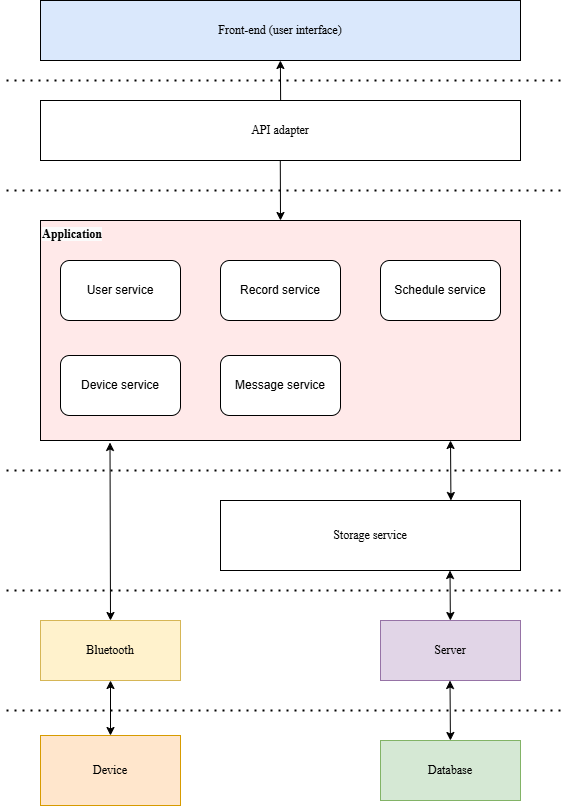
\includegraphics[width=12cm,height=14cm]{Images/System/fmECG_architecture-Patient-App.drawio.png}
  \caption[Sơ đồ khối application dành cho bệnh nhân]{\bfseries \fontsize{12pt}{0pt}\selectfont Sơ đồ khối ứng dụng di động dành cho bệnh nhân}
  \label{fmECG_architecture-Patient-App} %đặt tên cho ảnh
\end{figure}
Tầng trên cùng trong sơ đồ hình \ref{fmECG_architecture-Patient-App} là User Interface (Giao diện người dùng), nơi bệnh nhân trực tiếp tương tác với hệ thống thông qua API Adapter để gửi yêu cầu và nhận phản hồi.
Các yêu cầu này được xử lý bởi các Services chính, bao gồm User Service, Device Service, Record Service, Schedule Service, Diagnosis Service, Notification Service và Storage Service.

Những Services này được thiết kế nhằm đáp ứng các nhu cầu của bệnh nhân, từ quản lý thông tin cá nhân, mượn và trả thiết bị, theo dõi lịch sử dữ liệu phiên đo, cho đến việc quản lý lịch khám,
tra cứu thông tin chẩn đoán cho từng lịch khám. Ngoài ra, hệ thống còn đảm bảo việc gửi thông báo nhắc nhở kịp thời và hỗ trợ bệnh nhân trao đổi thông tin với bác sĩ một cách liền mạch và hiệu quả.

\subsubsection{Application dành cho bác sĩ}
\begin{figure}[H]
  \centering
  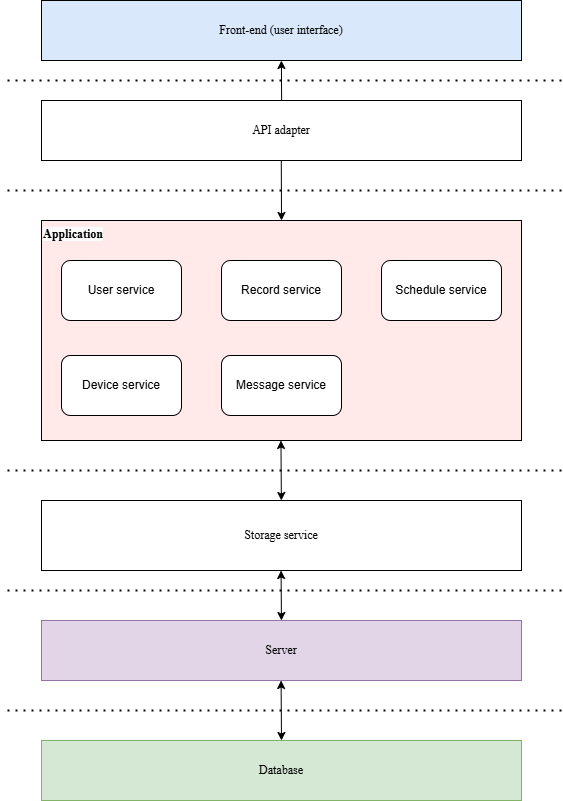
\includegraphics[width=12cm,height=14cm]{Images/System/fmECG_architecture-Doctors.drawio.png}
  \caption[Sơ đồ khối application dành cho bác sĩ]{\bfseries \fontsize{12pt}{0pt}\selectfont Sơ đồ khối ứng dụng di động dành cho bác sĩ}
  \label{fmECG_architecture-Doctor} %đặt tên cho ảnh
\end{figure}
Tương tự với bệnh nhân, sơ đồ hình \ref{fmECG_architecture-Doctor} được xây dựng để hỗ trợ bác sĩ thực hiện các nhiệm vụ chuyên môn thông qua giao diện người dùng và API Adapter, đảm bảo việc xử lý thông tin diễn ra nhanh chóng và hiệu quả.

Các Services chính, bao gồm User Service, Device Service, Record Service, Schedule Service, Diagnosis Service, Notification Service và Storage Service, đóng vai trò quan trọng trong việc hỗ trợ bác sĩ.
Các nhiệm vụ được tập trung vào việc theo dõi và phân tích dữ liệu phiên đo từ bệnh nhân, quản lý lịch khám, chấp nhận hoặc từ chối yêu cầu đặt lịch, ghi nhận thông tin chẩn đoán, và trao đổi trực tiếp với bệnh nhân.
Hơn nữa, hệ thống cung cấp khả năng tự động gửi thông báo về lịch khám và nhắc nhở các cuộc khám sắp tới, giúp bác sĩ quản lý thời gian và công việc hiệu quả hơn.

Cách tiếp cận này không chỉ hỗ trợ bác sĩ tổ chức công việc thuận lợi mà còn góp phần nâng cao hiệu quả điều trị cho bệnh nhân.

\subsubsection{Website cho quản trị viên}
\begin{figure}[H]
  \centering
  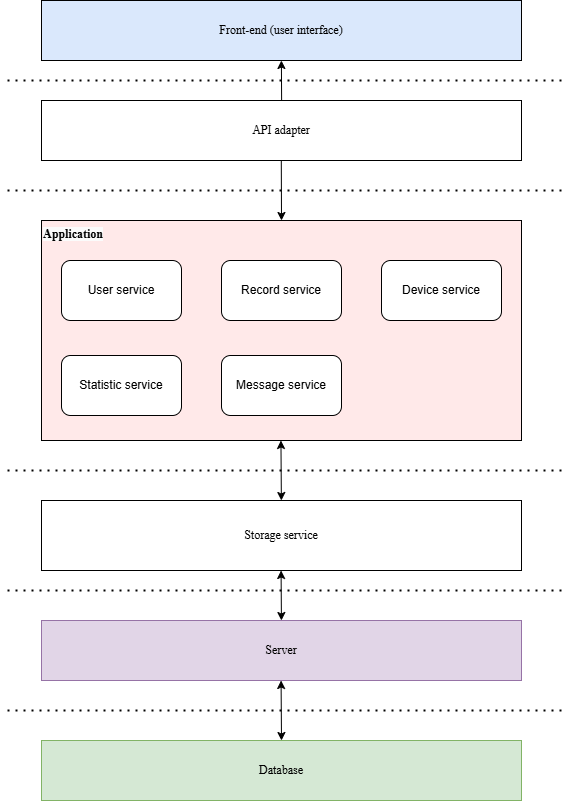
\includegraphics[width=12cm,height=14cm]{Images/System/fmECG_architecture-Admin.drawio.png}
  \caption[Sơ đồ khối Website dành cho quản trị viên]{\bfseries \fontsize{12pt}{0pt}\selectfont Sơ đồ khối Website dành cho quản trị viên}
  \label{fmECG_architecture-Admin} %đặt tên cho ảnh
\end{figure}
Về cơ bản, website dành cho admin có cấu trúc tương tự như website hay là app dành cho bác sĩ và bệnh nhân.
Admin sẽ có quyền quản lý toàn bộ thông tin người dùng, thiết bị, bản ghi.

\subsection{Thiết kế cơ sở dữ liệu}

\subsubsection{Chuyển đổi từ mô hình thực thể liên kết sang mô hình quan hệ}
Dựa trên bảng mô tả các thực thể và thuộc tính, chúng em tiến hành chuyển đổi từ mô hình thực thể liên kết thành mô hình quan hệ như sau.

\begin{itemize}
	\item Tài khoản đăng nhập (\textbf{ID tài khoản đăng nhập}, Địa chỉ email đăng ký, Mật khẩu truy cập)
	\item Token đăng nhập (\textbf{ID token đăng nhập}, ID tài khoản đăng nhập, Token làm mới, Hạn sử dụng, Trạng thái token)
	\item Vai trò người dùng (\textbf{ID vai trò}, Tên vai trò)
	\item Trạng thái hoạt động (\textbf{ID trạng thái người dùng}, Mô tả trạng thái người dùng)
	\item Người dùng (\textbf{ID người dùng}, ID tài khoản đăng nhập, ID vai trò người dùng, ID trạng thái hoạt động, Tên đầy đủ, Ngày tháng năm sinh, Giới tính, Số liên lạc, Đường dẫn ảnh đại diện, Thông tin bổ sung)
	\item Loại thiết bị (\textbf{ID loại thiết bị}, Tên loại thiết bị)
	\item Trạng thái thiết bị (\textbf{ID trạng thái thiết bị}, Mô tả trạng thái thiết bị)
	\item Thiết bị (\textbf{ID thiết bị}, ID người dùng thiết bị, ID loại thiết bị, ID trạng thái thiết bị, Tên thiết bị, Thông tin chi tiết về thiết bị, Ngày bắt đầu thời gian mượn, Ngày kết thúc thời gian mượn)
	\item Thông số kỹ thuật (\textbf{ID thông số kỹ thuật}, ID thiết bị, Loại thông số, Tên thông số, Giá trị thông số, Mô tả chi tiết thông số)
	\item Dữ liệu phiên đo (\textbf{ID dữ liệu phiên đo}, ID bệnh nhân, ID thiết bị, Loại bản ghi, Đường dẫn lưu trữ dữ liệu phiên đo, Thời gian bắt đầu thu thập dữ liệu, Thời gian kết thúc thu thập dữ liệu)
	\item Trạng thái lịch khám (\textbf{ID trạng thái lịch khám}, Mô tả trạng thái lịch khám)
	\item Kết quả lịch khám (\textbf{ID kết quả lịch khám}, Mô tả kết quả lịch khám)
	\item Lịch khám (\textbf{ID lịch khám}, ID bệnh nhân, ID bác sĩ, ID trạng thái lịch khám, ID kết quả lịch khám, Thời gian bắt đầu lịch khám, Thời gian kết thúc lịch khám)
	\item Thông báo liên quan đến lịch khám (\textbf{ID thông báo}, ID lịch khám, Loại thông báo, Nội dung thông báo, Trạng thái thông báo, Trạng thái đã xem, Lý do từ chối lịch khám)
	\item Chẩn đoán (\textbf{ID chẩn đoán}, ID lịch khám, Thông tin chẩn đoán)
	\item Tin nhắn (\textbf{ID tin nhắn}, ID người gửi, ID nhóm trò chuyện nhận tin nhắn, Nội dung tin nhắn, Thời gian gửi tin nhắn)
	\item Nhóm trò chuyện (\textbf{ID nhóm trò chuyện}, Tên nhóm trò chuyện, Người tạo nhóm, Danh sách thành viên nhóm, Sự kiện gửi tin nhắn, Sự kiện nhận tin nhắn)

\end{itemize}
\subsubsection{Chuẩn hoá 3NF}
Các bảng đã được thiết kế theo nguyên tắc chuẩn hoá 3NF, vì không có thuộc tính lặp lại và các thuộc tính không phụ thuộc vào một tập hợp con của khóa chính.

\paragraph{Chuẩn hoá bảng Tài khoản}
\mbox{}
\begin{table}[H]
	\caption{\bfseries \fontsize{12pt}{0pt}\selectfont Bảng chuẩn hoá bảng Tài khoản đăng nhập}
	\centering
	\begin{tabularx}{0.9\textwidth}{|X|X|}
		\hline
		\textbf{Danh sách thuộc tính} & ID tài khoản đăng nhập, Địa chỉ email đăng ký, Mật khẩu truy cập                                   \\
		\hline
		\textbf{Quy tắc nghiệp vụ}    & \textbf{Phụ thuộc hàm}                                                                             \\
		\hline
		Mỗi tài khoản có một ID riêng, có duy nhất Địa chỉ email đăng ký, Mật khẩu truy cập
		                              & \parbox[t]{\linewidth}{$\text{ID tài khoản} \rightarrow$ Địa chỉ email đăng ký, Mật khẩu truy cập} \\
		\hline
		\multicolumn{2}{|X|}{$\Rightarrow \text{Khoá chính của bảng: ID tài khoản đăng nhập}$}                                             \\
		\multicolumn{2}{|X|}{$\Rightarrow \text{Bảng Tài khoản đăng nhập đã ở 3NF}$}                                                       \\
		\hline
	\end{tabularx}
\end{table}

\paragraph{Chuẩn hoá bảng Token đăng nhập}
\mbox{}
\begin{table}[H]
	\caption{\bfseries \fontsize{12pt}{0pt}\selectfont Bảng chuẩn hoá bảng Token đăng nhập}
	\centering
	\begin{tabularx}{0.9\textwidth}{|X|X|}
		\hline
		\textbf{Danh sách thuộc tính} & ID token đăng nhập, ID tài khoản đăng nhập, Token làm mới, Hạn sử dụng, Trạng thái token                         \\
		\hline
		\textbf{Quy tắc nghiệp vụ}    & \textbf{Phụ thuộc hàm}                                                                                           \\
		\hline
		Mỗi tài khoản có một ID token riêng, có duy nhất ID tài khoản, Token làm mới, Hạn sử dụng, Trạng thái token
		                              & \parbox[t]{\linewidth}{$\text{ID token} \rightarrow$ ID tài khoản, Token làm mới, Hạn sử dụng, Trạng thái token} \\
		\hline
		\multicolumn{2}{|X|}{$\Rightarrow \text{Khoá chính của bảng: ID token đăng nhập}$}                                                               \\
		\multicolumn{2}{|X|}{$\Rightarrow \text{Bảng Token đăng nhập đã ở 3NF}$}                                                                         \\
		\hline
	\end{tabularx}
\end{table}

\paragraph{Chuẩn hoá bảng Vai trò người dùng}
\mbox{}
\begin{table}[H]
	\caption{\bfseries \fontsize{12pt}{0pt}\selectfont Bảng chuẩn hoá bảng Vai trò người dùng}
	\centering
	\begin{tabularx}{0.9\textwidth}{|X|X|}
		\hline
		\textbf{Danh sách thuộc tính} & ID vai trò, Tên vai trò                                             \\
		\hline
		\textbf{Quy tắc nghiệp vụ}    & \textbf{Phụ thuộc hàm}                                              \\
		\hline
		Mỗi vai trò có một ID riêng, có duy nhất Tên vai trò
		                              & \parbox[t]{\linewidth}{$\text{ID vai trò} \rightarrow$ Tên vai trò} \\
		\hline
		\multicolumn{2}{|X|}{$\Rightarrow \text{Khoá chính của bảng: ID vai trò}$}                          \\
		\multicolumn{2}{|X|}{$\Rightarrow \text{Bảng Vai trò người dùng đã ở 3NF}$}                         \\
		\hline
	\end{tabularx}
\end{table}

\paragraph{Chuẩn hoá bảng Trạng thái hoạt động}
\mbox{}
\begin{table}[H]
	\caption{\bfseries \fontsize{12pt}{0pt}\selectfont Bảng chuẩn hoá bảng Trạng thái hoạt động}
	\centering
	\begin{tabularx}{0.9\textwidth}{|X|X|}
		\hline
		\textbf{Danh sách thuộc tính} & ID trạng thái người dùng, Mô tả trạng thái người dùng                                             \\
		\hline
		\textbf{Quy tắc nghiệp vụ}    & \textbf{Phụ thuộc hàm}                                                                            \\
		\hline
		Mỗi trạng thái người dùng có một ID riêng, có duy nhất Mô tả trạng thái người dùng
		                              & \parbox[t]{\linewidth}{$\text{ID trạng thái người dùng} \rightarrow$ Mô tả trạng thái người dùng} \\
		\hline
		\multicolumn{2}{|X|}{$\Rightarrow \text{Khoá chính của bảng: ID trạng thái người dùng}$}                                          \\
		\multicolumn{2}{|X|}{$\Rightarrow \text{Bảng Trạng thái hoạt động đã ở 3NF}$}                                                     \\
		\hline
	\end{tabularx}
\end{table}

\paragraph{Chuẩn hoá bảng Người dùng}
\mbox{}
\begin{table}[H]
	\caption{\bfseries \fontsize{12pt}{0pt}\selectfont Bảng chuẩn hoá bảng Người dùng}
	\centering
	\begin{tabularx}{0.9\textwidth}{|X|X|}
		\hline
		\textbf{Danh sách thuộc tính}                                                                                                                                                                                          & ID người dùng, ID tài khoản đăng nhập, ID vai trò người dùng, ID trạng thái hoạt động, Tên đầy đủ, Ngày tháng năm sinh, Giới tính, Số liên lạc, Đường dẫn ảnh đại diện, Thông tin bổ sung                                             \\
		\hline
		\textbf{Quy tắc nghiệp vụ}                                                                                                                                                                                             & \textbf{Phụ thuộc hàm}                                                                                                                                                                                                                \\
		\hline
		Mỗi người dùng có một ID riêng, có duy nhất ID tài khoản đăng nhập, ID vai trò người dùng, ID trạng thái hoạt động, Tên đầy đủ, Ngày tháng năm sinh, Giới tính, Số liên lạc, Đường dẫn ảnh đại diện, Thông tin bổ sung & \parbox[t]{\linewidth}{$\text{ID người dùng} \rightarrow$ ID tài khoản đăng nhập, ID vai trò người dùng, ID trạng thái hoạt động, Tên đầy đủ, Ngày tháng năm sinh, Giới tính, Số liên lạc, Đường dẫn ảnh đại diện, Thông tin bổ sung} \\
		\hline
		\multicolumn{2}{|X|}{$\Rightarrow \text{Khoá chính của bảng: ID người dùng}$}                                                                                                                                                                                                                                                                                                                                                                                  \\
		\multicolumn{2}{|X|}{$\Rightarrow \text{Bảng Người dùng đã ở 3NF}$}                                                                                                                                                                                                                                                                                                                                                                                            \\
		\hline
	\end{tabularx}
\end{table}

\paragraph{Chuẩn hoá bảng Loại thiết bị}
\mbox{}
\begin{table}[H]
	\caption{\bfseries \fontsize{12pt}{0pt}\selectfont Bảng chuẩn hoá bảng Loại thiết bị}
	\centering
	\begin{tabularx}{0.9\textwidth}{|X|X|}
		\hline
		\textbf{Danh sách thuộc tính} & ID loại thiết bị, Tên loại thiết bị                                             \\
		\hline
		\textbf{Quy tắc nghiệp vụ}    & \textbf{Phụ thuộc hàm}                                                          \\
		\hline
		Mỗi loại thiết bị có một ID riêng, có duy nhất Tên loại thiết bị
		                              & \parbox[t]{\linewidth}{$\text{ID loại thiết bị} \rightarrow$ Tên loại thiết bị} \\
		\hline
		\multicolumn{2}{|X|}{$\Rightarrow \text{Khoá chính của bảng: ID loại thiết bị}$}                                \\
		\multicolumn{2}{|X|}{$\Rightarrow \text{Bảng loại thiết bị đã ở 3NF}$}                                          \\
		\hline
	\end{tabularx}
\end{table}

\paragraph{Chuẩn hoá bảng Trạng thái thiết bị}
\mbox{}
\begin{table}[H]
	\caption{\bfseries \fontsize{12pt}{0pt}\selectfont Bảng chuẩn hoá bảng Trạng thái thiết bị}
	\centering
	\begin{tabularx}{0.9\textwidth}{|X|X|}
		\hline
		\textbf{Danh sách thuộc tính} & ID trạng thái thiết bị, Mô tả trạng thái thiết bị                                             \\
		\hline
		\textbf{Quy tắc nghiệp vụ}    & \textbf{Phụ thuộc hàm}                                                                        \\
		\hline
		Mỗi trạng thái thiết bị có một ID riêng, có duy nhất Mô tả trạng thái thiết bị
		                              & \parbox[t]{\linewidth}{$\text{ID trạng thái thiết bị} \rightarrow$ Mô tả trạng thái thiết bị} \\
		\hline
		\multicolumn{2}{|X|}{$\Rightarrow \text{Khoá chính của bảng: ID trạng thái thiết bị}$}                                        \\
		\multicolumn{2}{|X|}{$\Rightarrow \text{Bảng Trạng thái thiết bị đã ở 3NF}$}                                                  \\
		\hline
	\end{tabularx}
\end{table}

\paragraph{Chuẩn hoá bảng Thiết bị}
\mbox{}
\begin{table}[H]
	\caption{\bfseries \fontsize{12pt}{0pt}\selectfont Bảng chuẩn hoá bảng Thiết bị}
	\centering
	\begin{tabularx}{0.9\textwidth}{|X|X|}
		\hline
		\textbf{Danh sách thuộc tính} & ID thiết bị, ID người dùng thiết bị, Tên thiết bị, Thông tin chi tiết về thiết bị, Ngày bắt đầu thời gian mượn, Ngày kết thúc thời gian mượn \\
		\hline
		\textbf{Quy tắc nghiệp vụ}    & \textbf{Phụ thuộc hàm}                                                                                                                       \\
		\hline
		Mỗi thiết bị có một ID thiết bị riêng, có duy nhất tên thiết bị, loại thiết bị, thông tin thiết bị,
		ID người dùng thiết bị, trạng thái thiết bị, ngày bắt đầu sử dụng, ngày kết thúc sử dụng
		                              & \parbox[t]{\linewidth}{$\text{ID thiết bị} \rightarrow$ ID người dùng thiết bị, Tên thiết bị,
		Loại thiết bị, Thông tin thiết bị, Trạng thái thiết bị, Ngày bắt đầu sử dụng, Ngày kết thúc sử dụng}                                                                         \\
		\hline
		\multicolumn{2}{|X|}{$\Rightarrow \text{Khoá chính của bảng: ID thiết bị}$}                                                                                                  \\
		\multicolumn{2}{|X|}{$\Rightarrow \text{Bảng Thiết bị đã ở 3NF}$}                                                                                                            \\
		\hline
	\end{tabularx}
\end{table}

\paragraph{Chuẩn hoá bảng Thông số kỹ thuật}
\mbox{}
\begin{table}[H]
	\caption{\bfseries \fontsize{12pt}{0pt}\selectfont Bảng chuẩn hoá bảng Thông số kỹ thuật}
	\centering
	\begin{tabularx}{0.9\textwidth}{|X|X|}
		\hline
		\textbf{Danh sách thuộc tính} & ID thông số kỹ thuật, ID thiết bị, Loại thông số, Tên thông số, Giá trị thông số, Mô tả chi tiết thông số                                             \\
		\hline
		\textbf{Quy tắc nghiệp vụ}    & \textbf{Phụ thuộc hàm}                                                                                                                                \\
		\hline
		Mỗi thông số kỹ thuật sẽ có một ID riêng, có duy nhất ID thiết bị, Loại thông số, Tên thông số, Giá trị thông số, Mô tả chi tiết thông số
		                              & \parbox[t]{\linewidth}{$\text{ID thông số kỹ thuật} \rightarrow$ ID thiết bị, Loại thông số, Tên thông số, Giá trị thông số, Mô tả chi tiết thông số} \\
		\hline
		\multicolumn{2}{|X|}{$\Rightarrow \text{Khoá chính của bảng: ID thông số kỹ thuật}$}                                                                                                  \\
		\multicolumn{2}{|X|}{$\Rightarrow \text{Bảng Thông số kỹ thuật đã ở 3NF}$}                                                                                                            \\
		\hline
	\end{tabularx}
\end{table}

\paragraph{Chuẩn hoá bảng Dữ liệu phiên đo}
\mbox{}
\begin{table}[H]
	\caption{\bfseries \fontsize{12pt}{0pt}\selectfont Bảng chuẩn hoá bảng Dữ liệu phiên đo}
	\centering
	\begin{tabularx}{0.9\textwidth}{|X|X|}
		\hline
		\textbf{Danh sách thuộc tính} & ID dữ liệu phiên đo, ID bệnh nhân, ID thiết bị, Loại bản ghi, Đường dẫn lưu trữ dữ liệu phiên đo, Thời gian bắt đầu thu thập dữ liệu, Thời gian kết thúc thu thập dữ liệu                                             \\
		\hline
		\textbf{Quy tắc nghiệp vụ}    & \textbf{Phụ thuộc hàm}                                                                                                                                                                                                \\
		\hline
		Mỗi dữ liệu phiên đo có một ID riêng, có duy nhất ID bệnh nhân, ID thiết bị, Loại bản ghi, Đường dẫn lưu trữ dữ liệu phiên đo, Thời gian bắt đầu thu thập dữ liệu, Thời gian kết thúc thu thập dữ liệu
		                              & \parbox[t]{\linewidth}{$\text{ID dữ liệu phiên đo} \rightarrow$ ID bệnh nhân, ID thiết bị, Loại bản ghi, Đường dẫn lưu trữ dữ liệu phiên đo, Thời gian bắt đầu thu thập dữ liệu, Thời gian kết thúc thu thập dữ liệu} \\
		\hline
		\multicolumn{2}{|X|}{$\Rightarrow \text{Khoá chính của bảng: ID dữ liệu phiên đo}$}                                                                                                                                                                   \\
		\multicolumn{2}{|X|}{$\Rightarrow \text{Bảng Dữ liệu phiên đo đã ở 3NF}$}                                                                                                                                                                             \\
		\hline
	\end{tabularx}
\end{table}

\paragraph{Chuẩn hoá bảng Trạng thái lịch khám}
\mbox{}
\begin{table}[H]
	\caption{\bfseries \fontsize{12pt}{0pt}\selectfont Bảng chuẩn hoá bảng Trạng thái lịch khám}
	\centering
	\begin{tabularx}{0.9\textwidth}{|X|X|}
		\hline
		\textbf{Danh sách thuộc tính} & ID trạng thái lịch khám, Mô tả trạng thái lịch khám                                             \\
		\hline
		\textbf{Quy tắc nghiệp vụ}    & \textbf{Phụ thuộc hàm}                                                                          \\
		\hline
		Mỗi trạng thái lịch khám có một ID riêng, có duy nhất Mô tả trạng thái lịch khám
		                              & \parbox[t]{\linewidth}{$\text{ID trạng thái lịch khám} \rightarrow$ Mô tả trạng thái lịch khám} \\
		\hline
		\multicolumn{2}{|X|}{$\Rightarrow \text{Khoá chính của bảng: ID trạng thái lịch khám}$}                                         \\
		\multicolumn{2}{|X|}{$\Rightarrow \text{Bảng Trạng thái lịch khám đã ở 3NF}$}                                                   \\
		\hline
	\end{tabularx}
\end{table}

\paragraph{Chuẩn hoá bảng Kết quả lịch khám}
\mbox{}
\begin{table}[H]
	\caption{\bfseries \fontsize{12pt}{0pt}\selectfont Bảng chuẩn hoá bảng Kết quả lịch khám}
	\centering
	\begin{tabularx}{0.9\textwidth}{|X|X|}
		\hline
		\textbf{Danh sách thuộc tính} & ID kết quả lịch khám, Mô tả kết quả lịch khám                                             \\
		\hline
		\textbf{Quy tắc nghiệp vụ}    & \textbf{Phụ thuộc hàm}                                                                    \\
		\hline
		Mỗi Kết quả lịch khám có một ID riêng, có duy nhất Mô tả kết quả lịch khám
		                              & \parbox[t]{\linewidth}{$\text{ID kết quả lịch khám} \rightarrow$ Mô tả kết quả lịch khám} \\
		\hline
		\multicolumn{2}{|X|}{$\Rightarrow \text{Khoá chính của bảng: ID kết quả lịch khám}$}                                      \\
		\multicolumn{2}{|X|}{$\Rightarrow \text{Bảng Kết quả lịch khám đã ở 3NF}$}                                                \\
		\hline
	\end{tabularx}
\end{table}

\paragraph{Chuẩn hoá bảng Lịch khám}
\mbox{}
\begin{table}[H]
	\caption{\bfseries \fontsize{12pt}{0pt}\selectfont Bảng chuẩn hoá bảng Lịch khám}
	\centering
	\begin{tabularx}{0.9\textwidth}{|X|X|}
		\hline
		\textbf{Danh sách thuộc tính} & ID lịch khám, ID bệnh nhân, ID bác sĩ, ID trạng thái lịch khám, ID kết quả lịch khám, Thời gian bắt đầu lịch khám, Thời gian kết thúc lịch khám                                             \\
		\hline
		\textbf{Quy tắc nghiệp vụ}    & \textbf{Phụ thuộc hàm}                                                                                                                                                                      \\
		\hline
		Mỗi Lịch khám có một ID riêng, có duy nhất ID bệnh nhân, ID bác sĩ, ID trạng thái lịch khám, ID kết quả lịch khám, Thời gian bắt đầu lịch khám, Thời gian kết thúc lịch khám
		                              & \parbox[t]{\linewidth}{$\text{ID lịch khám} \rightarrow$ ID bệnh nhân, ID bác sĩ, ID trạng thái lịch khám, ID kết quả lịch khám, Thời gian bắt đầu lịch khám, Thời gian kết thúc lịch khám} \\
		\hline
		\multicolumn{2}{|X|}{$\Rightarrow \text{Khoá chính của bảng: ID  lịch khám}$}                                                                                                                                               \\
		\multicolumn{2}{|X|}{$\Rightarrow \text{Bảng Lịch khám đã ở 3NF}$}                                                                                                                                                          \\
		\hline
	\end{tabularx}
\end{table}

\paragraph{Chuẩn hoá bảng Thông báo liên quan đến lịch khám}
\mbox{}
\begin{table}[H]
	\caption{\bfseries \fontsize{12pt}{0pt}\selectfont Bảng chuẩn hoá bảng Thông báo liên quan đến lịch khám}
	\centering
	\begin{tabularx}{0.9\textwidth}{|X|X|}
		\hline
		\textbf{Danh sách thuộc tính} & ID thông báo, ID lịch khám, Loại thông báo, Nội dung thông báo, Trạng thái thông báo, Trạng thái đã xem, Lý do từ chối lịch khám                                             \\
		\hline
		\textbf{Quy tắc nghiệp vụ}    & \textbf{Phụ thuộc hàm}                                                                                                                                                       \\
		\hline
		Mỗi Thông báo liên quan đến lịch khám có một ID riêng, có duy nhất ID lịch khám, Loại thông báo, Nội dung thông báo, Trạng thái thông báo, Trạng thái đã xem, Lý do từ chối lịch khám
		                              & \parbox[t]{\linewidth}{$\text{ID thông báo} \rightarrow$ ID lịch khám, Loại thông báo, Nội dung thông báo, Trạng thái thông báo, Trạng thái đã xem, Lý do từ chối lịch khám} \\
		\hline
		\multicolumn{2}{|X|}{$\Rightarrow \text{Khoá chính của bảng: ID  thông báo}$}                                                                                                                                \\
		\multicolumn{2}{|X|}{$\Rightarrow \text{Bảng Thông báo liên quan đến lịch khám đã ở 3NF}$}                                                                                                                   \\
		\hline
	\end{tabularx}
\end{table}

\paragraph{Chuẩn hoá bảng Chẩn đoán}
\mbox{}
\begin{table}[H]
	\caption{\bfseries \fontsize{12pt}{0pt}\selectfont Bảng chuẩn hoá bảng Chẩn đoán}
	\centering
	\begin{tabularx}{0.9\textwidth}{|X|X|}
		\hline
		\textbf{Danh sách thuộc tính} & ID chẩn đoán, ID lịch khám, Thông tin chẩn đoán                                             \\
		\hline
		\textbf{Quy tắc nghiệp vụ}    & \textbf{Phụ thuộc hàm}                                                                      \\
		\hline
		Mỗi Chẩn đoán có một ID riêng, có duy nhất ID lịch khám, Thông tin chẩn đoán
		                              & \parbox[t]{\linewidth}{$\text{ID chẩn đoán} \rightarrow$ ID lịch khám, Thông tin chẩn đoán} \\
		\hline
		\multicolumn{2}{|X|}{$\Rightarrow \text{Khoá chính của bảng: ID  chẩn đoán}$}                                               \\
		\multicolumn{2}{|X|}{$\Rightarrow \text{Bảng Chẩn đoán đã ở 3NF}$}                                                          \\
		\hline
	\end{tabularx}
\end{table}

\paragraph{Chuẩn hoá bảng Tin nhắn}
\mbox{}
\begin{table}[H]
	\caption{\bfseries \fontsize{12pt}{0pt}\selectfont Bảng chuẩn hoá bảng Tin nhắn}
	\centering
	\begin{tabularx}{0.9\textwidth}{|X|X|}
		\hline
		\textbf{Danh sách thuộc tính} & ID tin nhắn, ID người gửi, ID nhóm trò chuyện nhận tin nhắn, Nội dung tin nhắn, Thời gian gửi tin nhắn                                             \\
		\hline
		\textbf{Quy tắc nghiệp vụ}    & \textbf{Phụ thuộc hàm}                                                                                                                             \\
		\hline
		Mỗi Tin nhắn có một ID riêng, có duy nhất ID người gửi, ID nhóm trò chuyện nhận tin nhắn, Nội dung tin nhắn, Thời gian gửi tin nhắn
		                              & \parbox[t]{\linewidth}{$\text{ID tin nhắn} \rightarrow$ ID người gửi, ID nhóm trò chuyện nhận tin nhắn, Nội dung tin nhắn, Thời gian gửi tin nhắn} \\
		\hline
		\multicolumn{2}{|X|}{$\Rightarrow \text{Khoá chính của bảng: ID  tin nhắn}$}                                                                                                       \\
		\multicolumn{2}{|X|}{$\Rightarrow \text{Bảng Tin nhắn đã ở 3NF}$}                                                                                                                  \\
		\hline
	\end{tabularx}
\end{table}

\paragraph{Chuẩn hoá bảng Nhóm trò chuyện}
\mbox{}
\begin{table}[H]
	\caption{\bfseries \fontsize{12pt}{0pt}\selectfont Bảng chuẩn hoá bảng Nhóm trò chuyện}
	\centering
	\begin{tabularx}{0.9\textwidth}{|X|X|}
		\hline
		\textbf{Danh sách thuộc tính} & ID nhóm trò chuyện, Tên nhóm trò chuyện, Người tạo nhóm, Danh sách thành viên nhóm, Sự kiện gửi tin nhắn, Sự kiện nhận tin nhắn                                             \\
		\hline
		\textbf{Quy tắc nghiệp vụ}    & \textbf{Phụ thuộc hàm}                                                                                                                                                      \\
		\hline
		Mỗi Nhóm trò chuyện có một ID riêng, có duy nhất Tên nhóm trò chuyện, Người tạo nhóm, Danh sách thành viên nhóm, Sự kiện gửi tin nhắn, Sự kiện nhận tin nhắn
		                              & \parbox[t]{\linewidth}{$\text{ID nhóm trò chuyện} \rightarrow$ Tên nhóm trò chuyện, Người tạo nhóm, Danh sách thành viên nhóm, Sự kiện gửi tin nhắn, Sự kiện nhận tin nhắn} \\
		\hline
		\multicolumn{2}{|X|}{$\Rightarrow \text{Khoá chính của bảng: ID  nhóm trò chuyện}$}                                                                                                                         \\
		\multicolumn{2}{|X|}{$\Rightarrow \text{Bảng Nhóm trò chuyện đã ở 3NF}$}                                                                                                                                    \\
		\hline
	\end{tabularx}
\end{table}

\subsubsection{Sơ đồ ERD}

\begin{figure}[H]
	\centering
	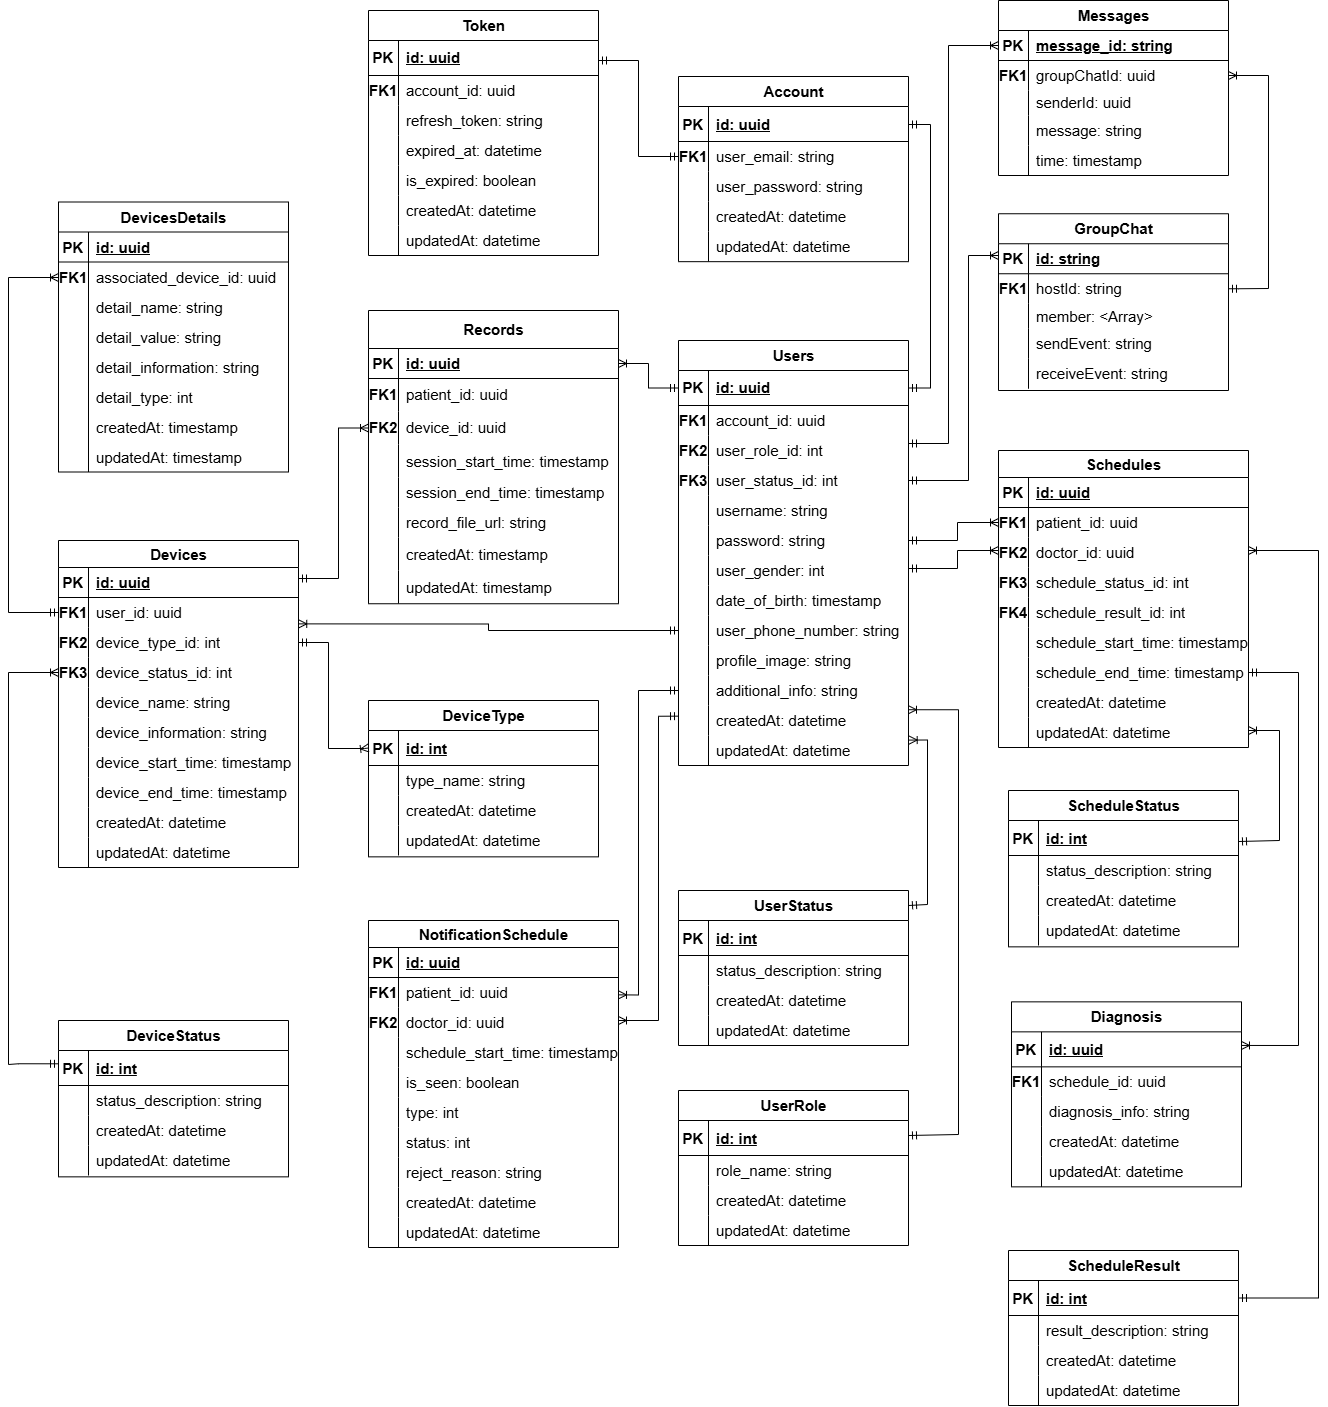
\includegraphics[width=15cm,height=15cm]{Images/system/ERD-db-Page-2.drawio.png}
	\caption[Sơ đồ ERD]{\bfseries \fontsize{12pt}{0pt}\selectfont Sơ đồ ERD}
	\label{fmECG_architecture-Database}
\end{figure}

\subsection{Thiết kế giao diện}

% Ứng dụng được thiết kế với giao diện hiện đại, sử dụng tông màu chủ đạo là trắng và xanh dương, mang lại cảm giác trang nhã và chuyên nghiệp, đồng thời phù hợp với hình ảnh đặc trưng của lĩnh vực y tế. Sự kết hợp này không chỉ tạo ấn tượng về sự tin cậy mà còn mang đến trải nghiệm người dùng dễ chịu, thân thiện.

% Dưới đây là các giao diện được em thiết kế trong App: 
% \begin{figure}[H]
% 	\centering
% 	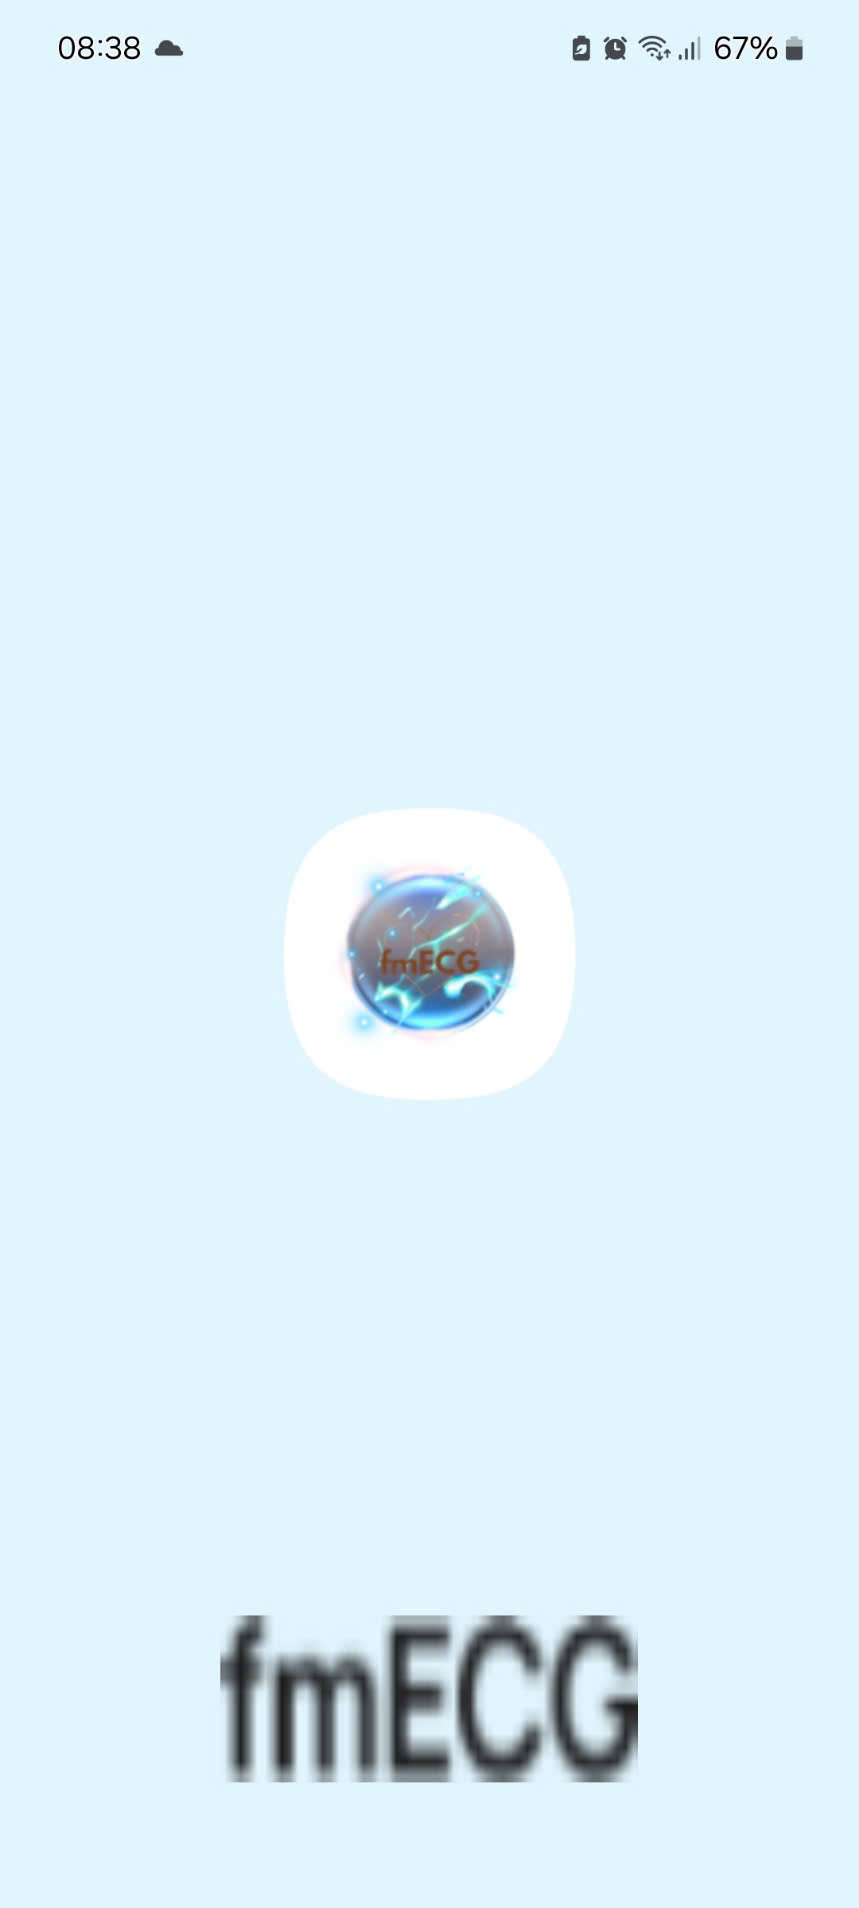
\includegraphics[width=8.5cm,height=18cm]{Images/AppUI/startApp.jpg}
% 	\caption[Giao diện khởi động app]{\bfseries \fontsize{12pt}{0pt}\selectfont Giao diện khởi động app}
% 	\label{startApp}
% \end{figure}
% Hình ảnh hiển thị biểu tượng chính của ứng dụng với nền màu xanh nhạt, mang lại cảm giác nhẹ nhàng và thân thiện với người dùng. Biểu tượng trung tâm là một quả cầu năng lượng với dòng chữ "fmECG," được tô điểm bằng hiệu ứng ánh sáng động, tượng trưng cho sự liên kết giữa công nghệ và y học hiện đại.
% \begin{figure}[H]
% 	\centering
% 	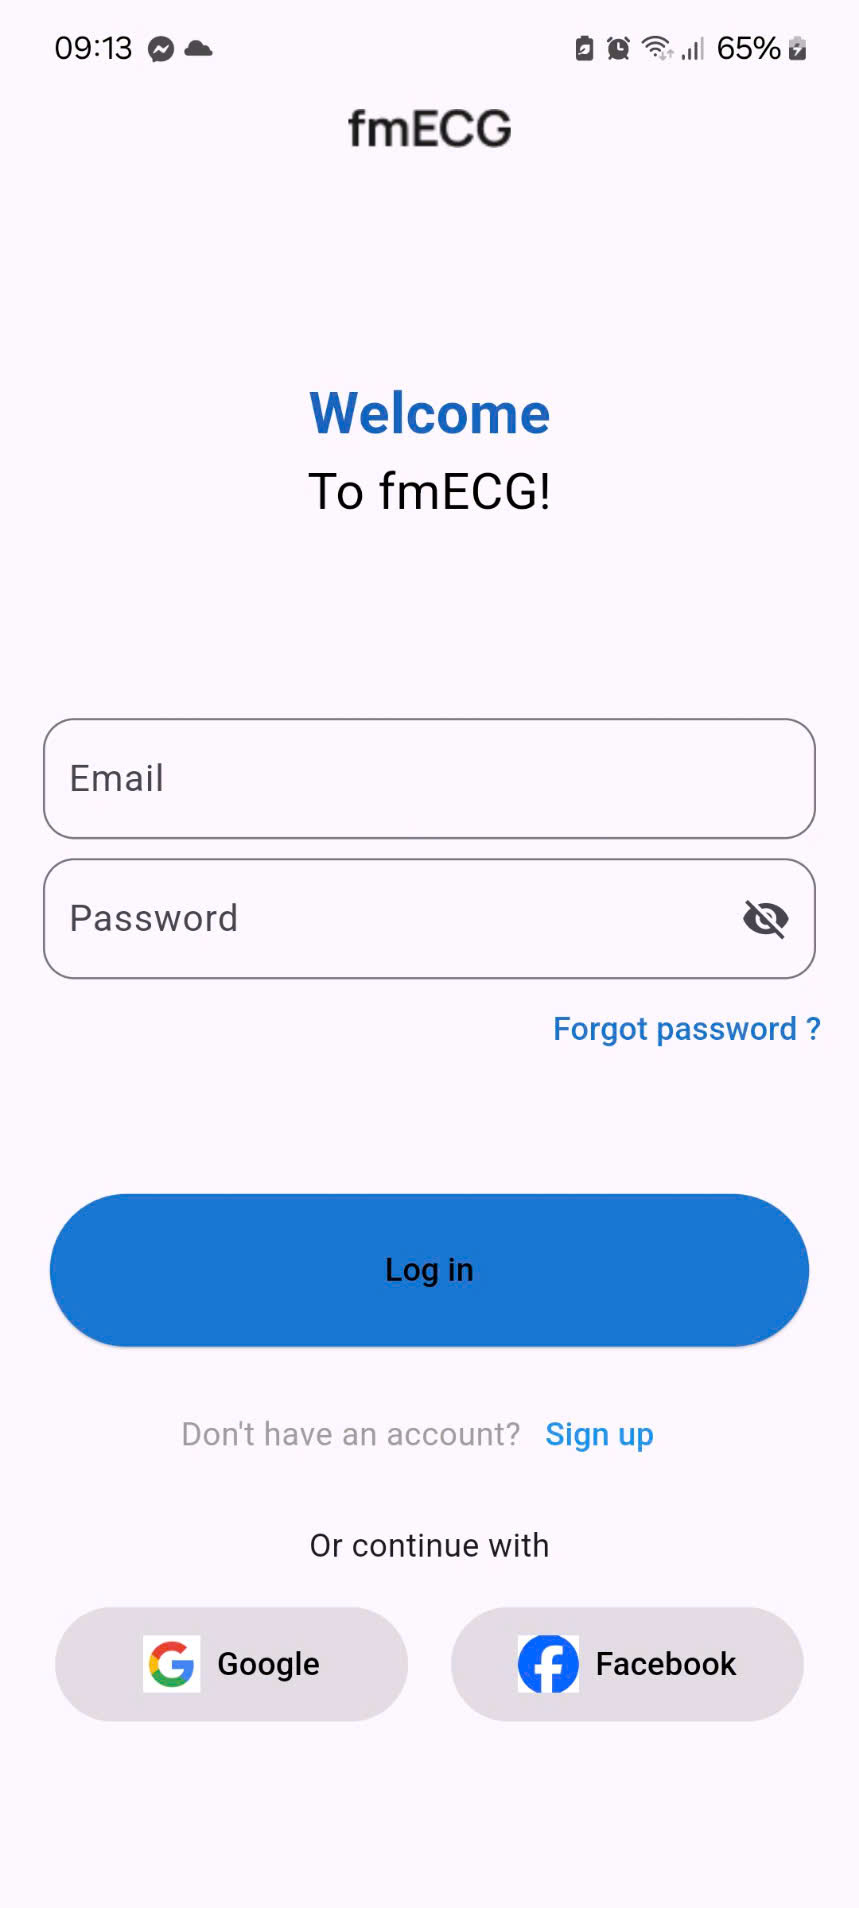
\includegraphics[width=8.5cm,height=18cm]{Images/AppUI/login.jpg}
% 	\caption[Giao diện trang đăng nhập]{\bfseries \fontsize{12pt}{0pt}\selectfont Giao diện trang đăng nhập}
% 	\label{login}
% \end{figure}
% Giao diện đăng nhập của ứng dụng "fmECG" được thiết kế đơn giản và thân thiện với người dùng. Ở phía trên cùng, tên ứng dụng "fmECG" được hiển thị rõ ràng, giúp người dùng dễ dàng nhận diện thương hiệu. Phía dưới là thông điệp chào mừng "Welcome to fmECG!" nhằm tạo cảm giác thân thiện và chuyên nghiệp. Giao diện cung cấp hai ô nhập thông tin: một ô dành cho "Email" và một ô cho "Password," với biểu tượng mắt đi kèm để hỗ trợ người dùng kiểm tra mật khẩu đã nhập.

% \begin{figure}[H] \centering 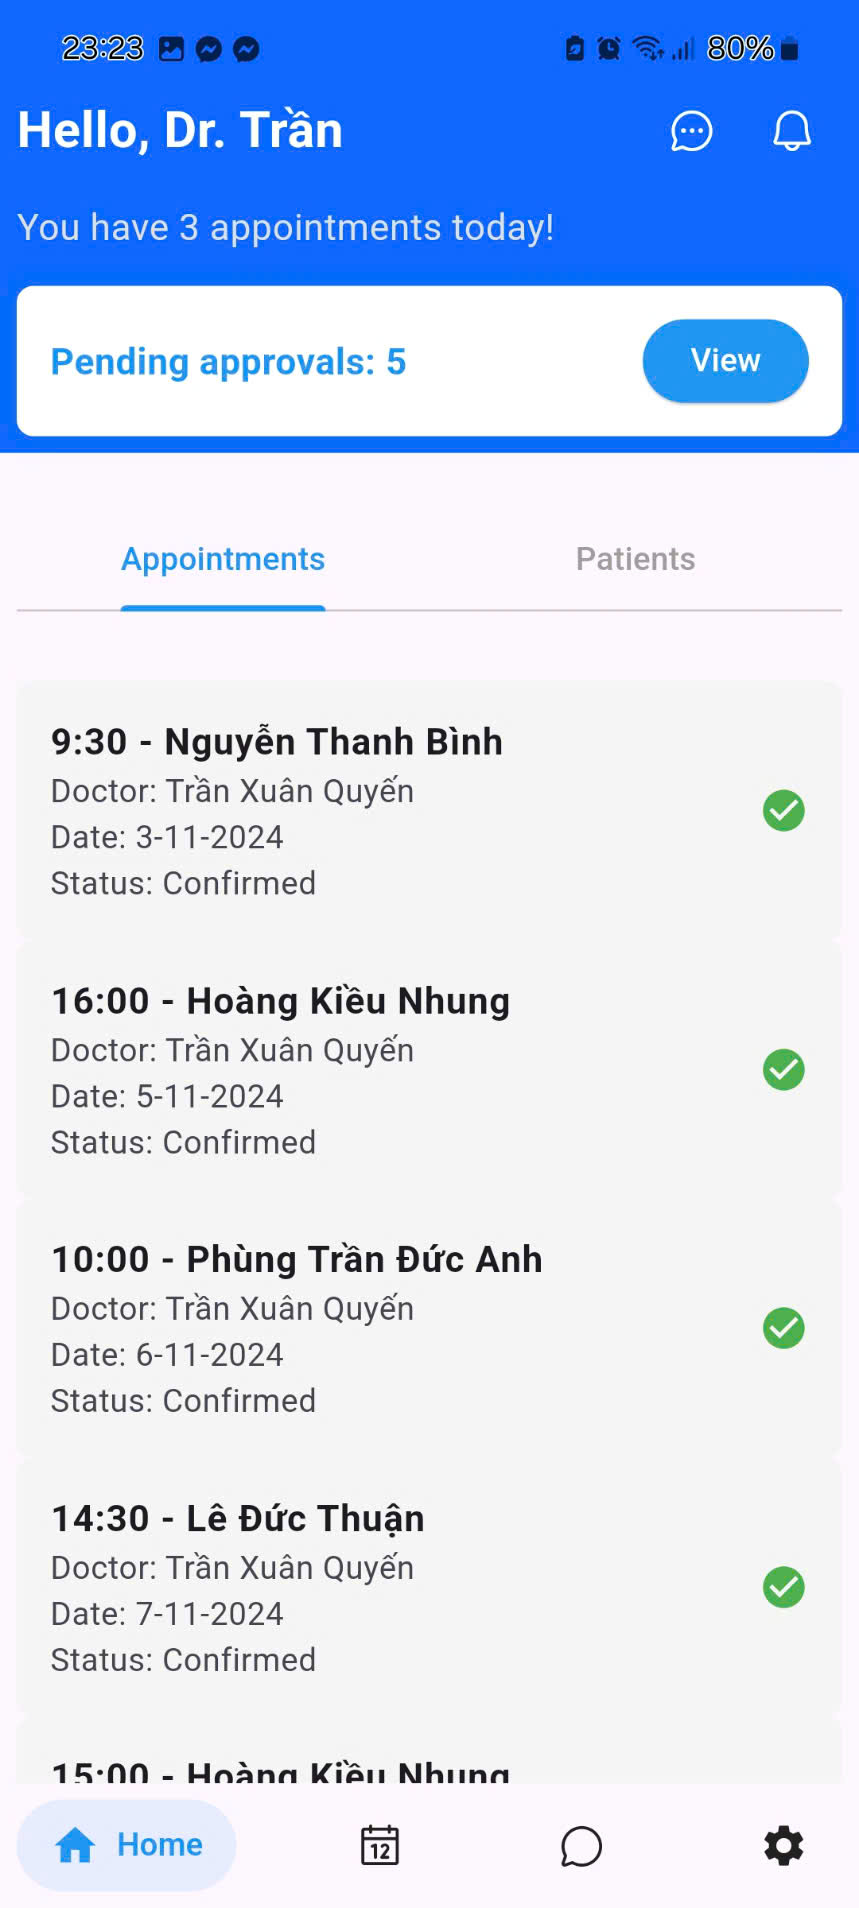
\includegraphics[width=8.5cm,height=18cm]{Images/AppUI/homePage1Doctor.jpg} \caption[Giao diện trang chủ của bác sĩ]{\bfseries \fontsize{12pt}{0pt}\selectfont Giao diện trang chủ của bác sĩ} \label{homeDoctor} \end{figure} 
% Trang chủ của bác sĩ được thiết kế để cung cấp thông tin tổng quan nhanh chóng và rõ ràng. Phần trên cùng hiển thị lời chào cá nhân hóa với số lượng cuộc hẹn trong ngày, đi kèm hai biểu tượng tin nhắn và thông báo ở góc phải để bác sĩ dễ dàng theo dõi thông tin quan trọng. Ngoài ra, mục "Pending approvals" hiển thị số yêu cầu đang chờ xử lý với nút "View" để chuyển hướng đến chi tiết. Phần dưới là danh sách các cuộc hẹn đã xác nhận, bao gồm thông tin thời gian, bệnh nhân, và trạng thái.

% \begin{figure}[H] \centering 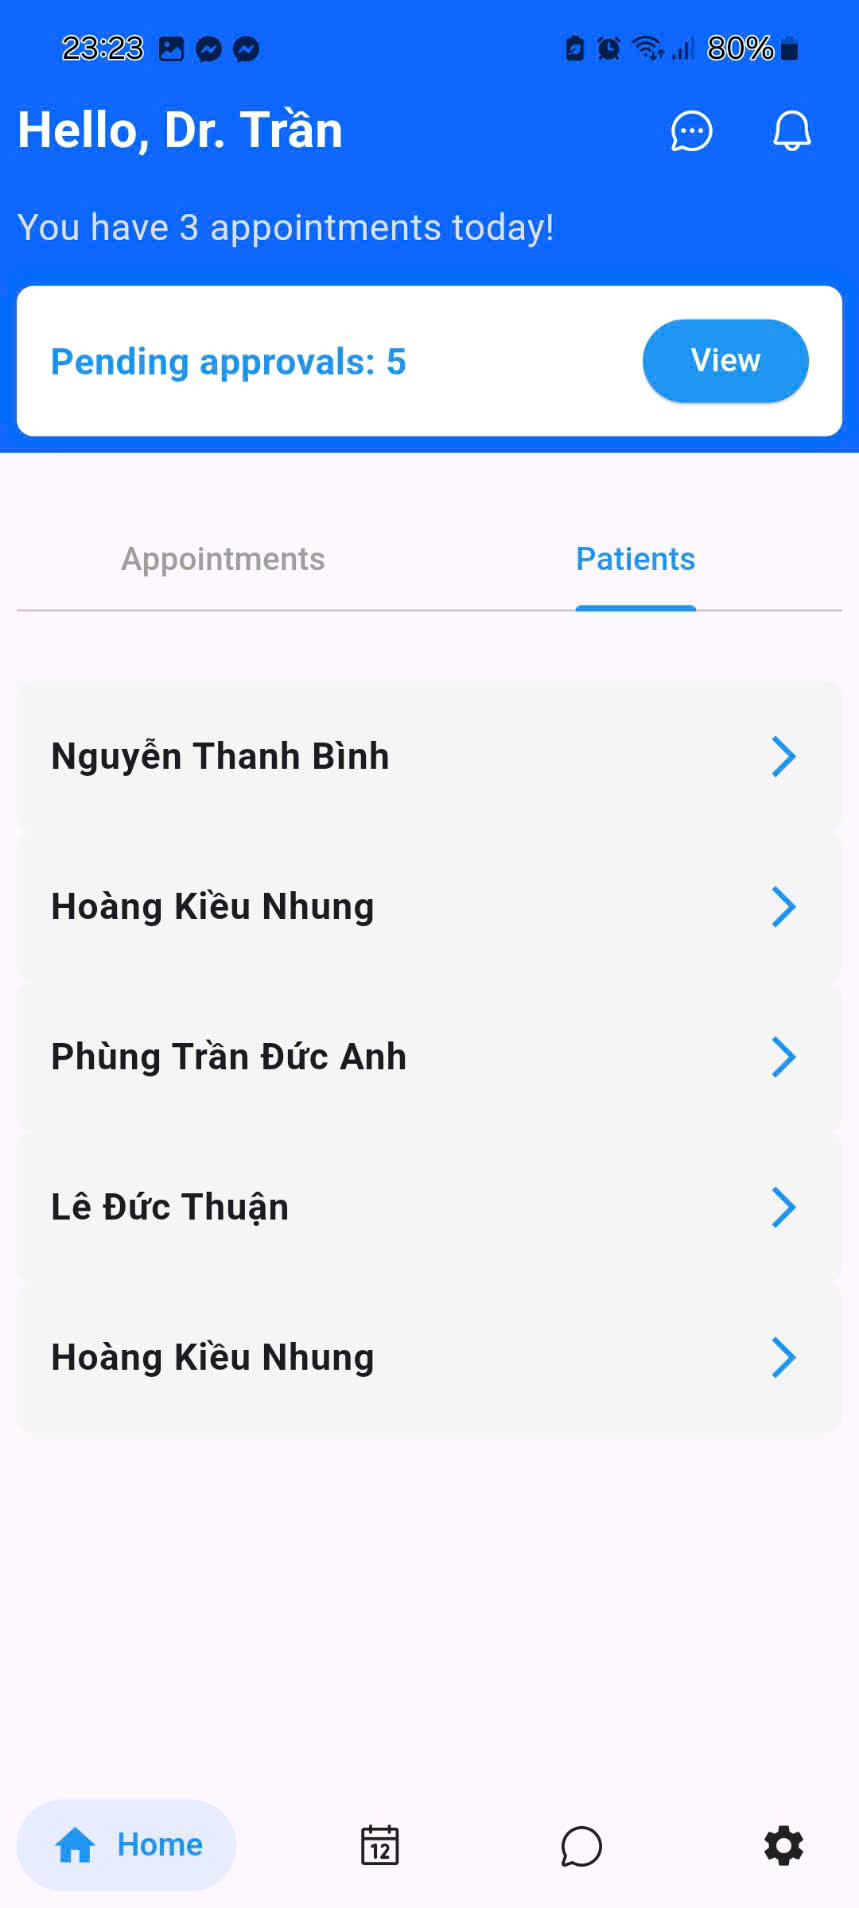
\includegraphics[width=8.5cm,height=18cm]{Images/AppUI/homePage2Doctor.jpg} \caption[Giao diện danh sách bệnh nhân của bác sĩ]{\bfseries \fontsize{12pt}{0pt}\selectfont Giao diện danh sách bệnh nhân của bác sĩ} \label{patientListDoctor} \end{figure} 
% Tab "Patients" trong giao diện bác sĩ hiển thị danh sách các bệnh nhân dưới dạng các mục riêng biệt. Mỗi mục bao gồm tên bệnh nhân cùng nút điều hướng để truy cập nhanh vào hồ sơ chi tiết của từng người. Thiết kế này giúp bác sĩ dễ dàng quản lý và theo dõi thông tin bệnh nhân của mình.

% \begin{figure}[H] \centering 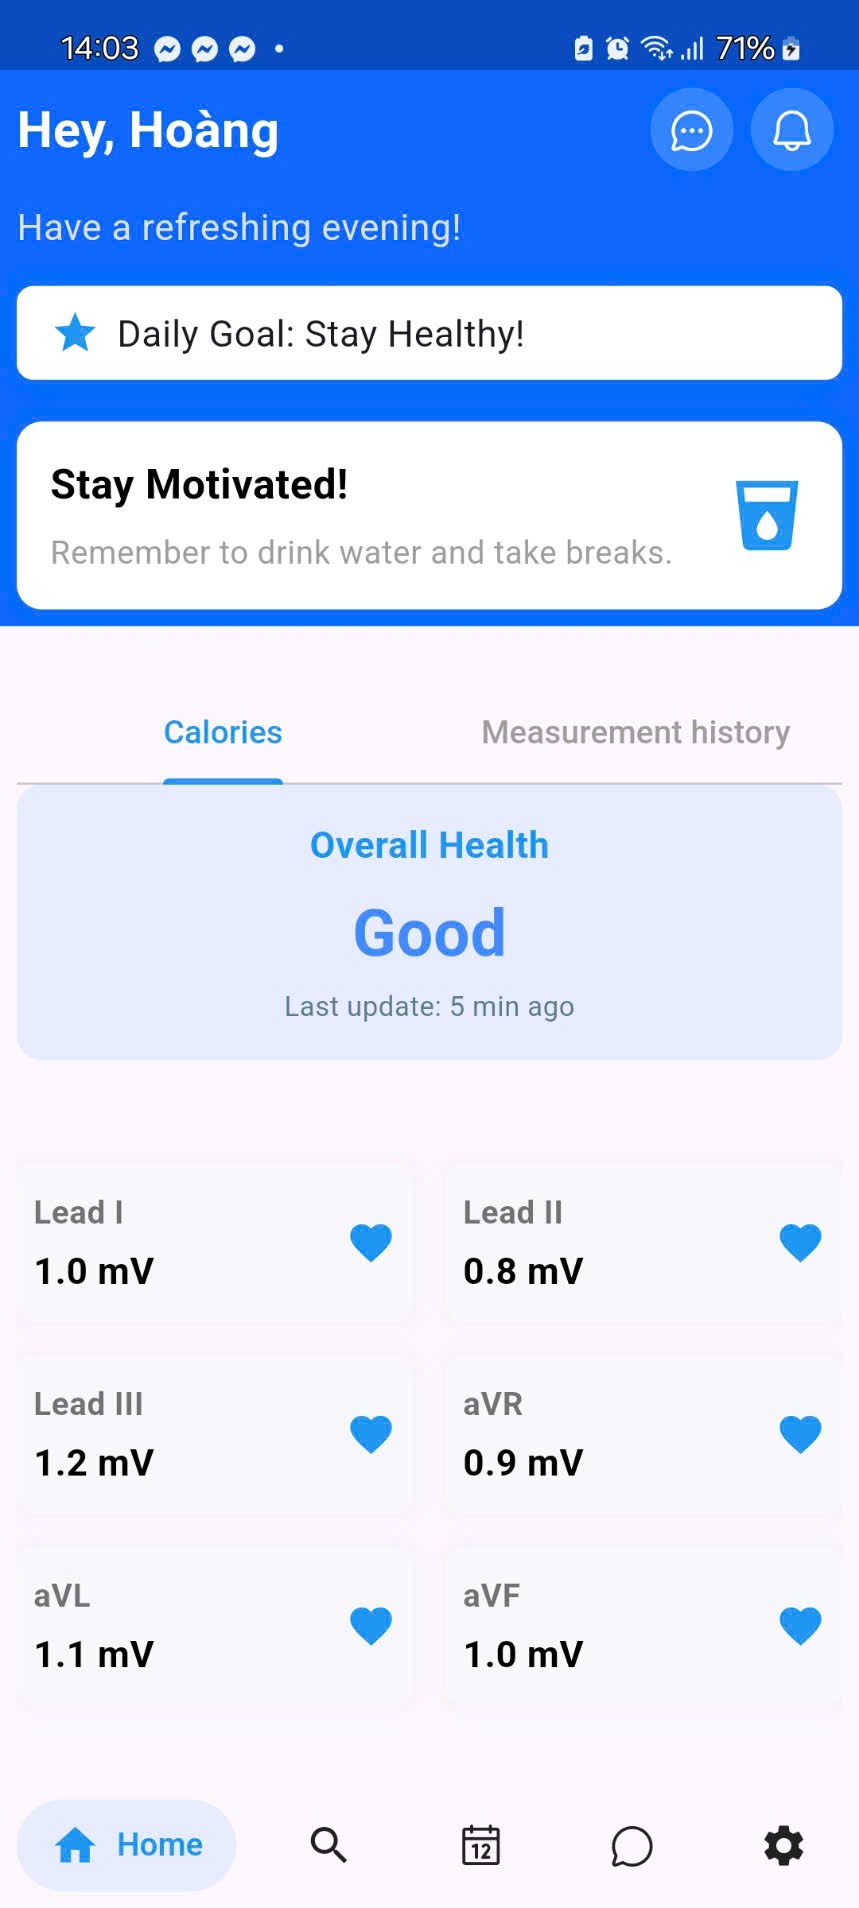
\includegraphics[width=8.5cm,height=18cm]{Images/AppUI/homePagePatient.jpg} \caption[Giao diện thông tin sức khỏe của bệnh nhân]{\bfseries \fontsize{12pt}{0pt}\selectfont Giao diện thông tin sức khỏe của bệnh nhân} \label{healthInfoPatient} \end{figure}
% Giao diện của bệnh nhân tập trung vào việc hiển thị trạng thái sức khỏe tổng quan với đánh giá "Overall Health: Good" được cập nhật gần nhất. Bên dưới là 6 số liệu liên quan đến điện tim, được trình bày rõ ràng và dễ hiểu. Những số liệu này đại diện cho các thông tin đo lường quan trọng, giúp bệnh nhân theo dõi tình trạng sức khỏe tim mạch của mình một cách trực quan. Giao diện hiện đại và thân thiện, mang đến trải nghiệm sử dụng thuận tiện và tối ưu.

% Sang giao diện đặt lịch:
% \begin{figure}[H]
% 	\centering
% 	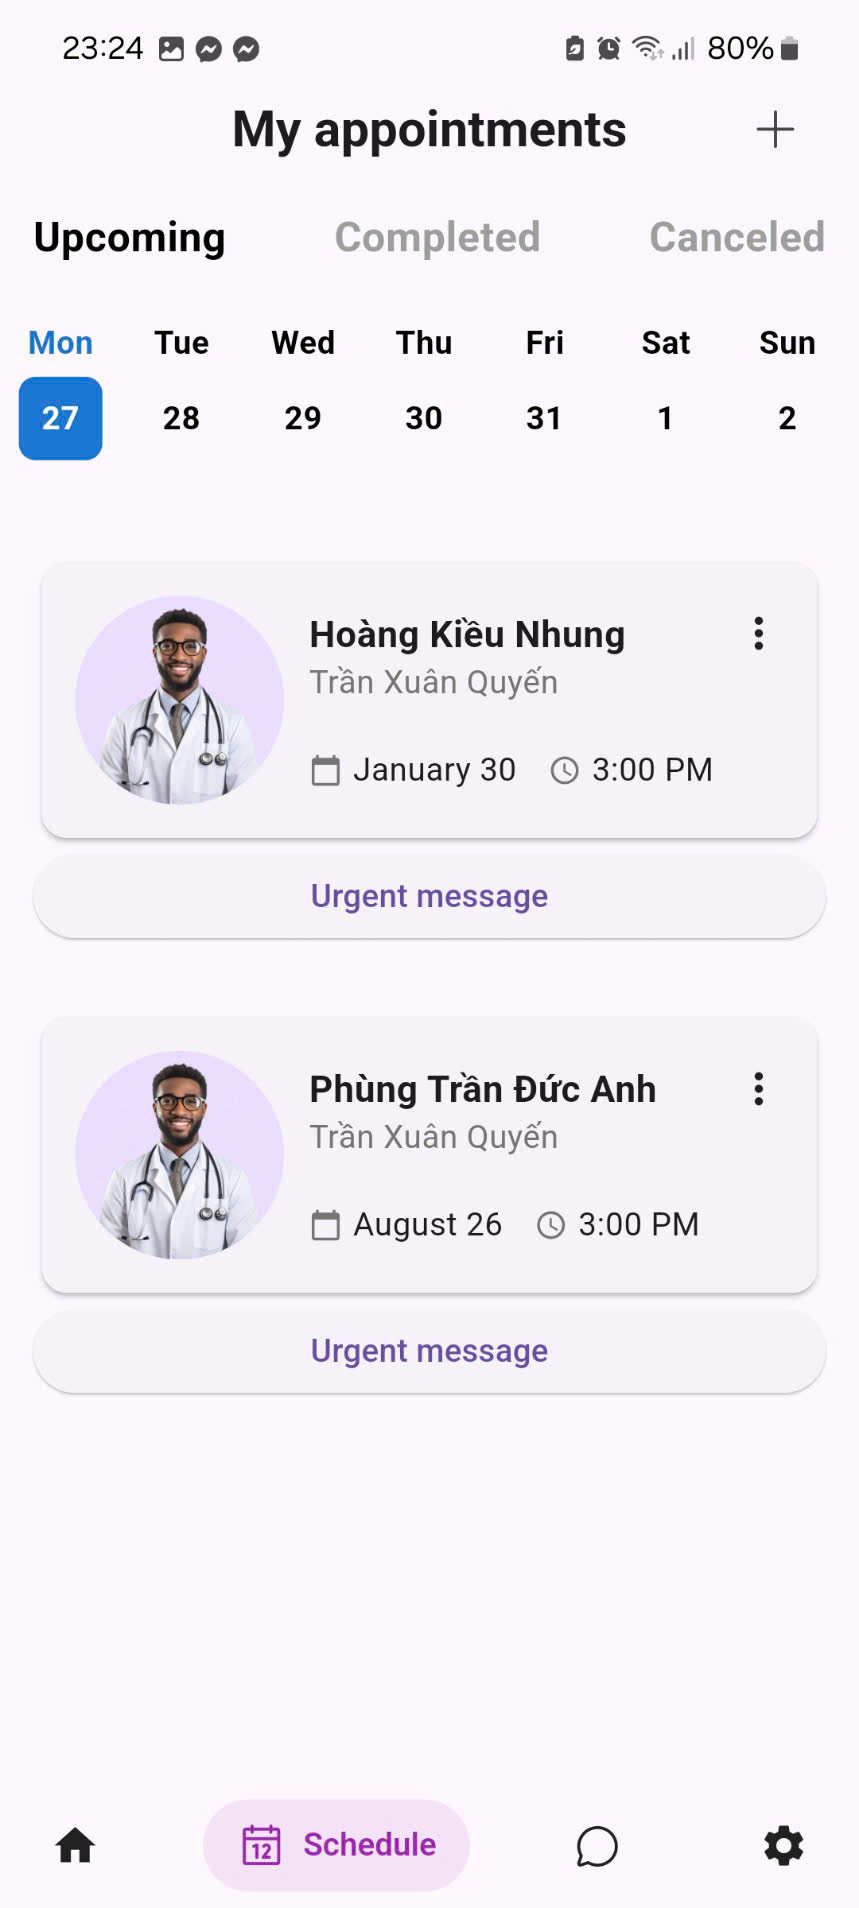
\includegraphics[width=8.5cm,height=18cm]{Images/AppUI/scheduleUpComing.jpg}
% 	\caption[Giao diện quản lý lịch của bác sĩ]{\bfseries \fontsize{12pt}{0pt}\selectfont Giao diện quản lý lịch của bác sĩ}
% 	\label{scheduleDoctor}
% \end{figure}
% Giao diện quản lý lịch của bác sĩ được chia thành ba tab chính: \textbf{Upcoming}, \textbf{Completed}, và \textbf{Canceled}. Tab \textbf{Upcoming} hiển thị danh sách các cuộc hẹn sắp tới với thông tin chi tiết như tên bệnh nhân, ngày và giờ hẹn, cùng nút "Urgent message" để liên lạc khẩn cấp khi cần thiết. 


% \begin{figure}[H]
% 	\centering
% 	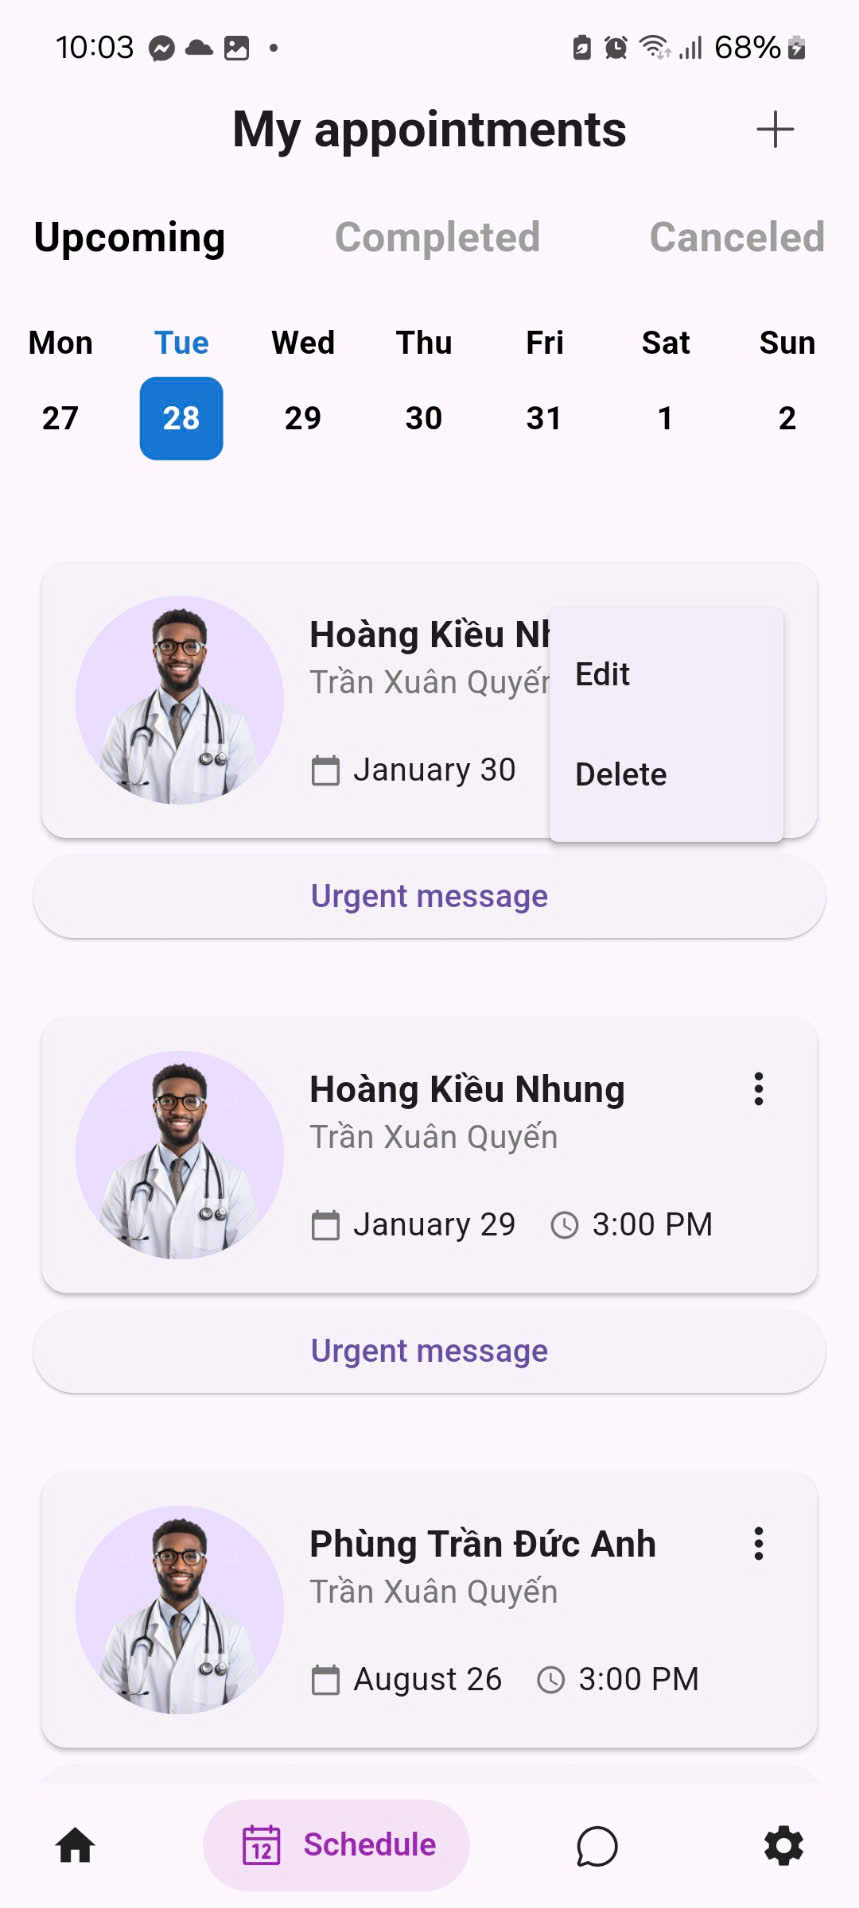
\includegraphics[width=8.5cm,height=18cm]{Images/AppUI/optionSchedule.jpg}
% 	\caption[Tùy chọn hủy lịch hẹn trong tab Upcoming]{\bfseries \fontsize{12pt}{0pt}\selectfont Tùy chọn hủy lịch hẹn trong tab Upcoming}
% 	\label{upcomingOptions}
% \end{figure}
% Trong tab \textbf{Upcoming}, mỗi cuộc hẹn đều có biểu tượng dấu ba chấm ở góc phải, cho phép bác sĩ truy cập vào các tùy chọn bổ sung. Một trong số đó là chức năng \textbf{Hủy lịch hẹn}. Khi nhấn vào tùy chọn này, một cửa sổ mới sẽ xuất hiện, yêu cầu bác sĩ nhập lý do hủy lịch.

% \begin{figure}[H]
% 	\centering
% 	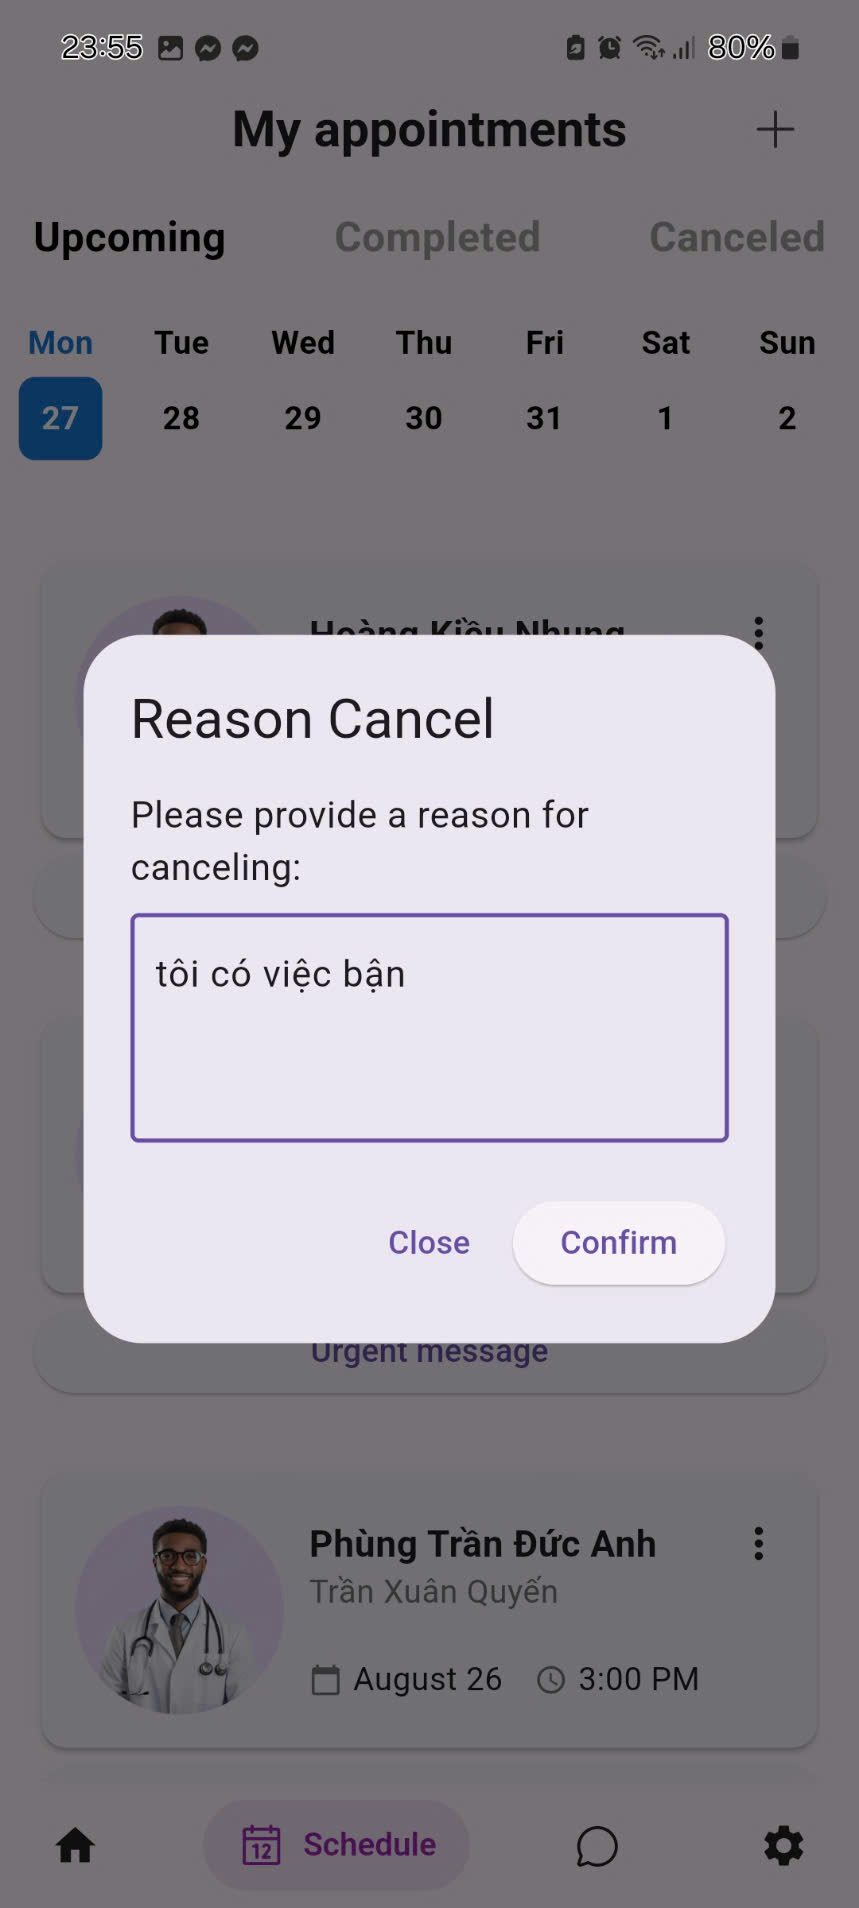
\includegraphics[width=8.5cm,height=18cm]{Images/AppUI/cancelledSchedule.jpg}
% 	\caption[Giao diện nhập lý do hủy lịch hẹn]{\bfseries \fontsize{12pt}{0pt}\selectfont Giao diện nhập lý do hủy lịch hẹn}
% 	\label{cancelAppointment}
% \end{figure}
% Giao diện nhập lý do hủy lịch hẹn cung cấp một ô nhập liệu để bác sĩ điền thông tin giải thích lý do hủy cuộc hẹn. Phía dưới là hai nút chức năng:
% \begin{itemize}
% 	\item \textbf{Cancel Appointment}: Xác nhận hủy lịch hẹn sau khi lý do được nhập.
% 	\item \textbf{Close}: Đóng cửa sổ mà không thực hiện thay đổi.
% \end{itemize}
% Chức năng này đảm bảo bác sĩ có thể quản lý lịch hẹn linh hoạt, đồng thời cung cấp thông tin rõ ràng cho bệnh nhân về lý do hủy lịch.


% Tab \textbf{Completed} tập hợp các cuộc hẹn đã hoàn thành. Khi nhấn vào một mục trong danh sách, bác sĩ sẽ được chuyển đến cửa sổ chi tiết, hiển thị thông tin bệnh nhân như tên, tuổi, giới tính, và số điện thoại, cùng với các tùy chọn thao tác như nhập thông tin chẩn đoán và tạo lịch tái khám. Tab \textbf{Canceled} cho phép bác sĩ theo dõi các cuộc hẹn đã bị hủy, hỗ trợ việc quản lý lịch sử làm việc dễ dàng hơn.

% \begin{figure}[H]
% 	\centering
% 	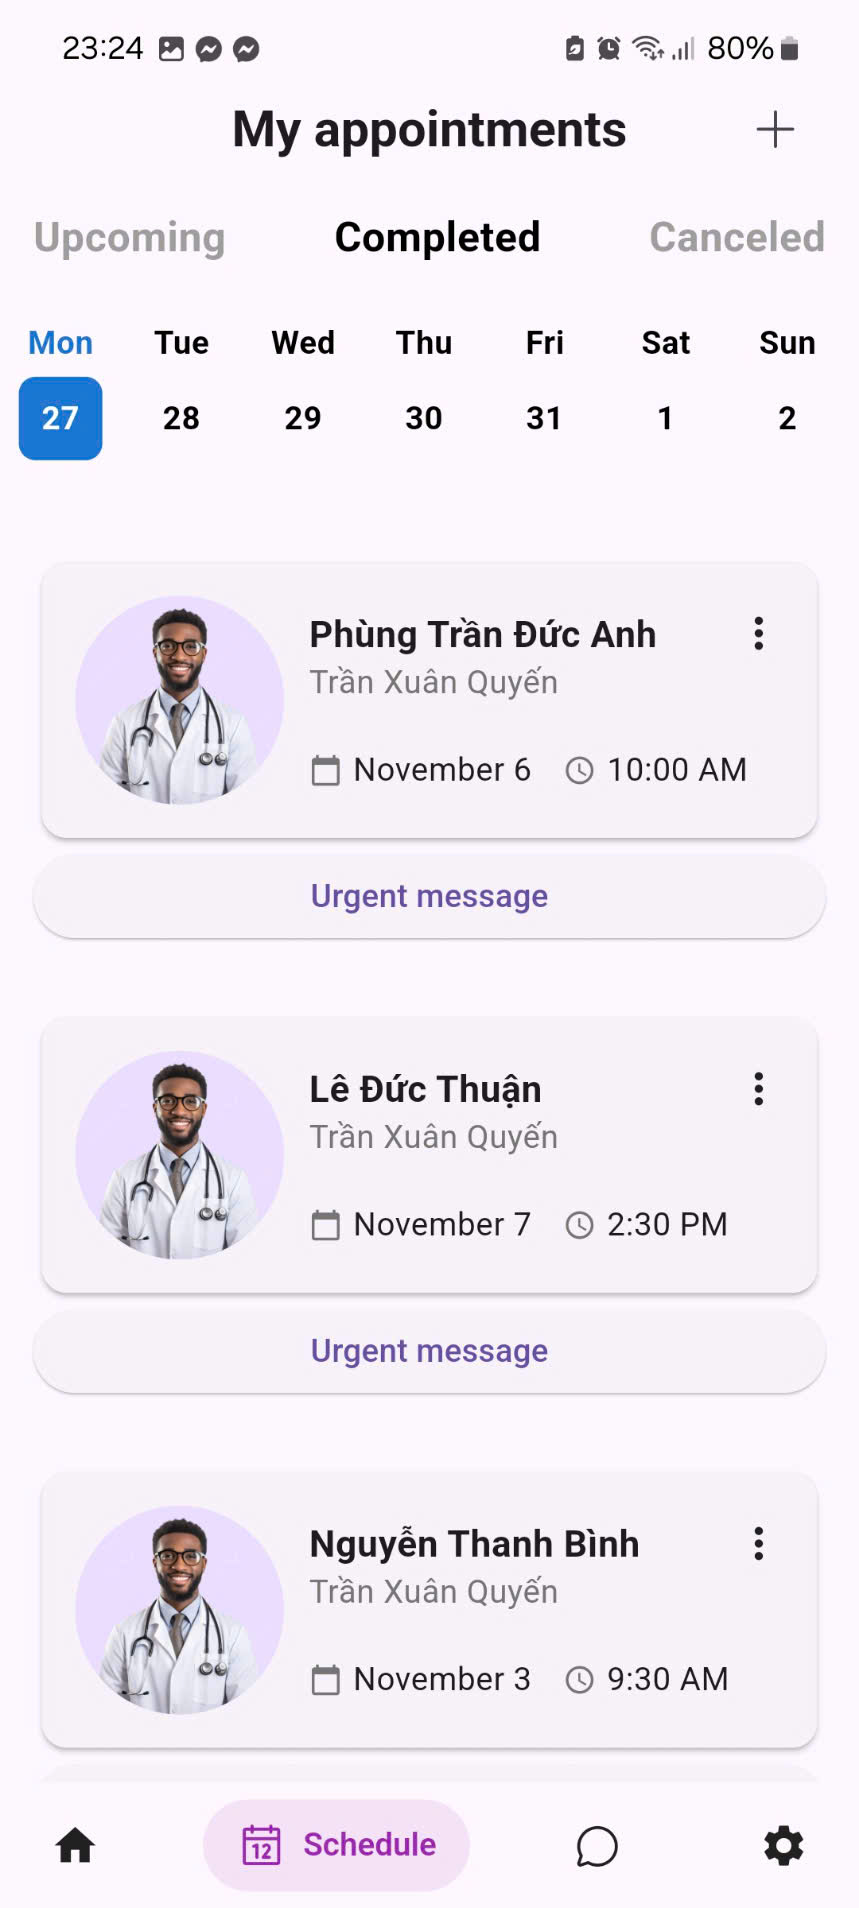
\includegraphics[width=8.5cm,height=18cm]{Images/AppUI/scheduleCompleted.jpg}
% 	\caption[Chi tiết thông tin bệnh nhân từ lịch đã hoàn thành]{\bfseries \fontsize{12pt}{0pt}\selectfont Chi tiết thông tin bệnh nhân từ lịch đã hoàn thành}
% 	\label{patientInfo}
% \end{figure}
% Khi truy cập vào thông tin chi tiết từ tab \textbf{Completed}, bác sĩ sẽ thấy toàn bộ thông tin về bệnh nhân, bao gồm tên, tuổi, giới tính, và số điện thoại. Bên dưới là các nút chức năng như:
% \begin{itemize}
% 	\item \textbf{Chẩn đoán}: Cho phép bác sĩ nhập hoặc chỉnh sửa thông tin chẩn đoán cho bệnh nhân.
% 	\item \textbf{Tạo lịch tái khám}: Hỗ trợ bác sĩ đặt lịch tái khám mới với giao diện chọn ngày và giờ trực quan.
% 	\item \textbf{Đóng cửa sổ}: Kết thúc thao tác và quay lại danh sách.
% \end{itemize}

% \begin{figure}[H]
% 	\centering
% 	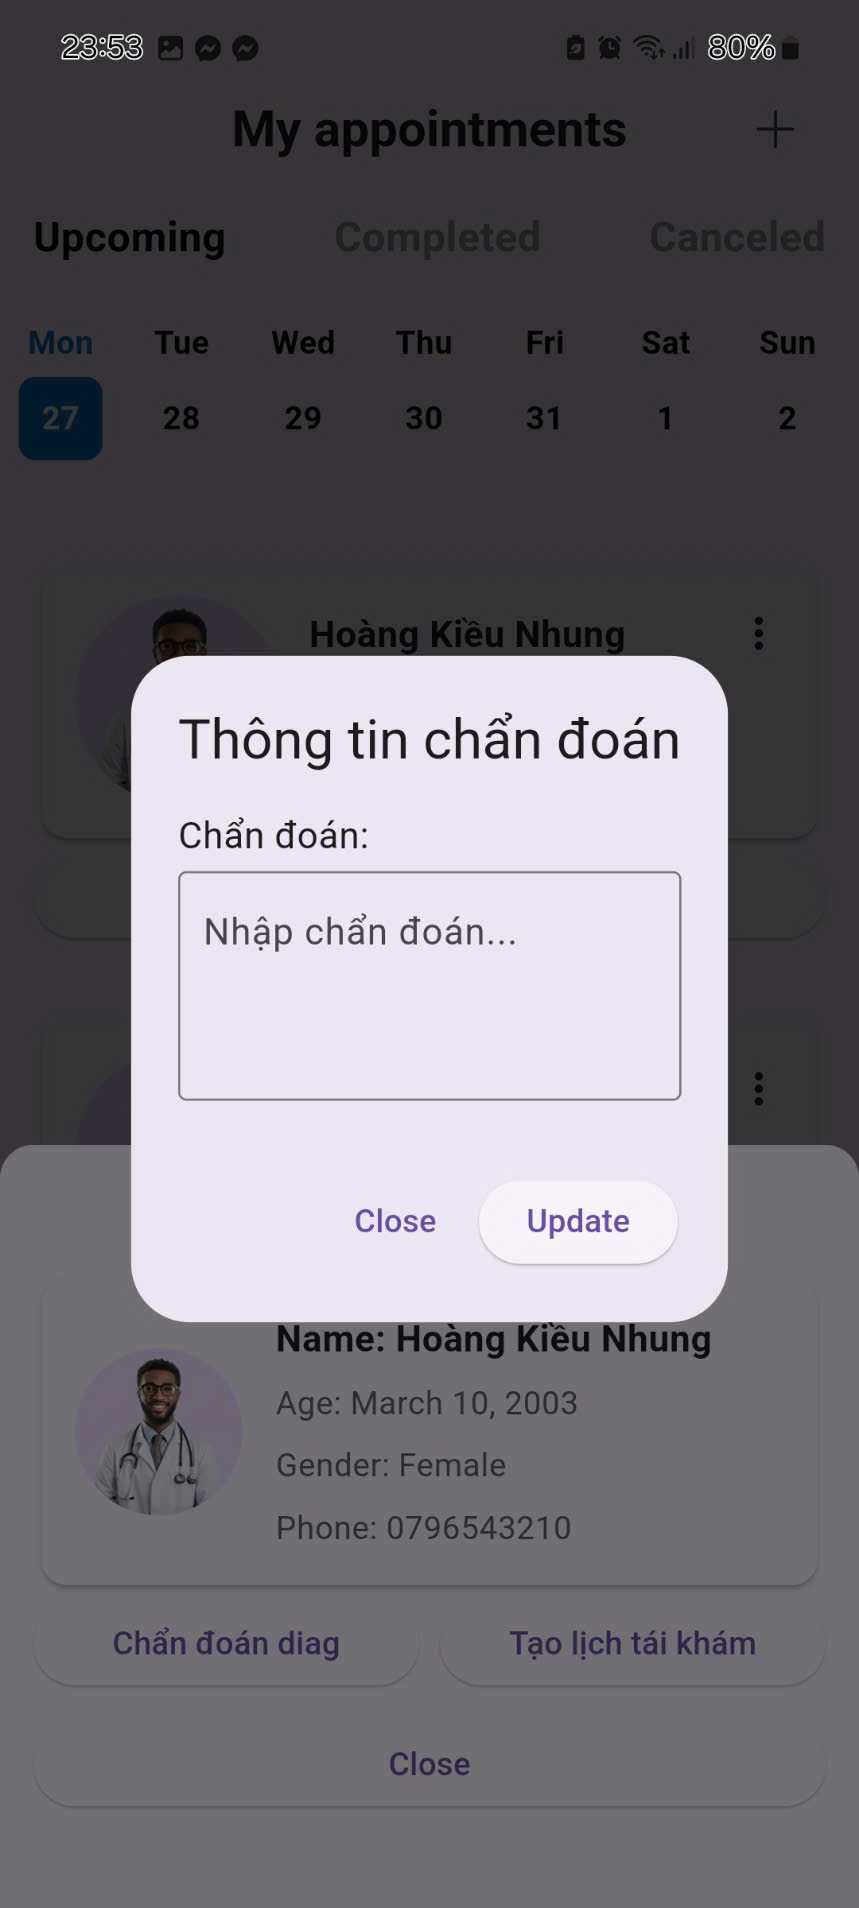
\includegraphics[width=8.5cm,height=18cm]{Images/AppUI/blockInputDIag.jpg}
% 	\caption[Cửa sổ cập nhật thông tin chẩn đoán]{\bfseries \fontsize{12pt}{0pt}\selectfont Cửa sổ cập nhật thông tin chẩn đoán}
% 	\label{diagnosisUpdate}
% \end{figure}
% Giao diện cập nhật chẩn đoán cung cấp một ô nhập liệu để bác sĩ thêm hoặc chỉnh sửa nội dung chẩn đoán, đi kèm nút \textbf{Update} để lưu thông tin mới.

% \begin{figure}[H]
% 	\centering
% 	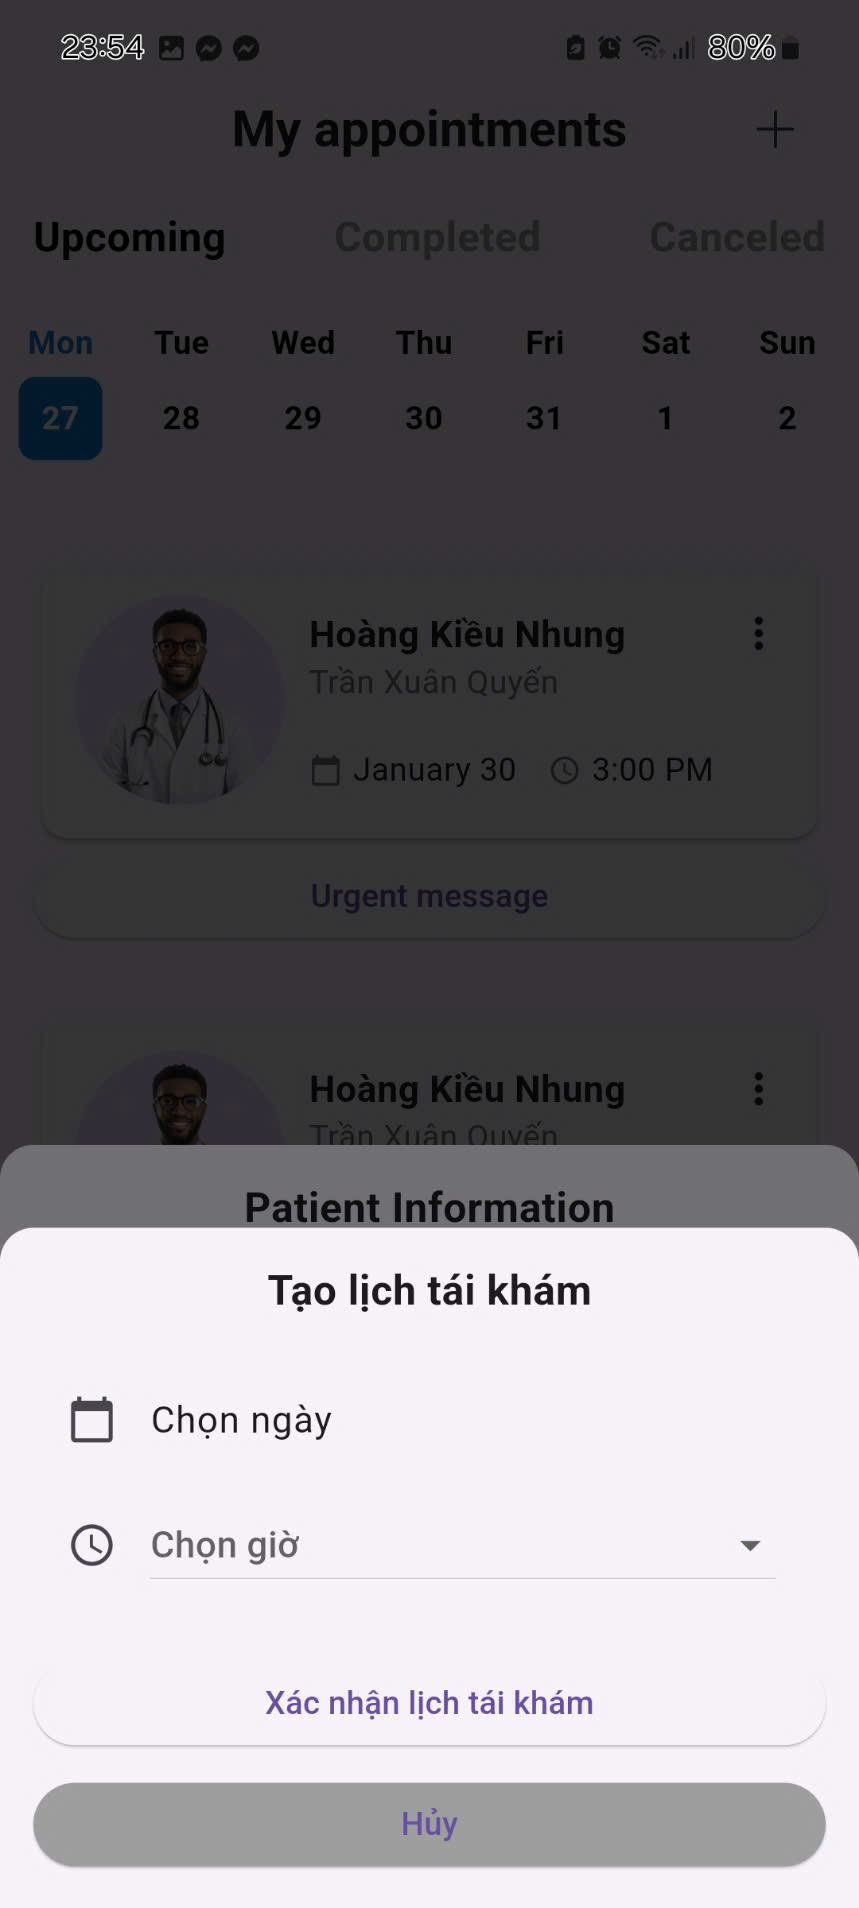
\includegraphics[width=8.5cm,height=18cm]{Images/AppUI/repickSchedule2.jpg}
% 	\caption[Cửa sổ tạo lịch tái khám]{\bfseries \fontsize{12pt}{0pt}\selectfont Cửa sổ tạo lịch tái khám}
% 	\label{reschedule}
% \end{figure}
% Giao diện đặt lịch tái khám cho phép bác sĩ chọn ngày và giờ, sau đó xác nhận bằng nút \textbf{Xác nhận lịch tái khám}. Điều này giúp đảm bảo việc quản lý các cuộc hẹn diễn ra mượt mà và hiệu quả.

\subsubsection{Màn hình khởi động và đăng nhập}

\begin{figure}[H]
	\centering
	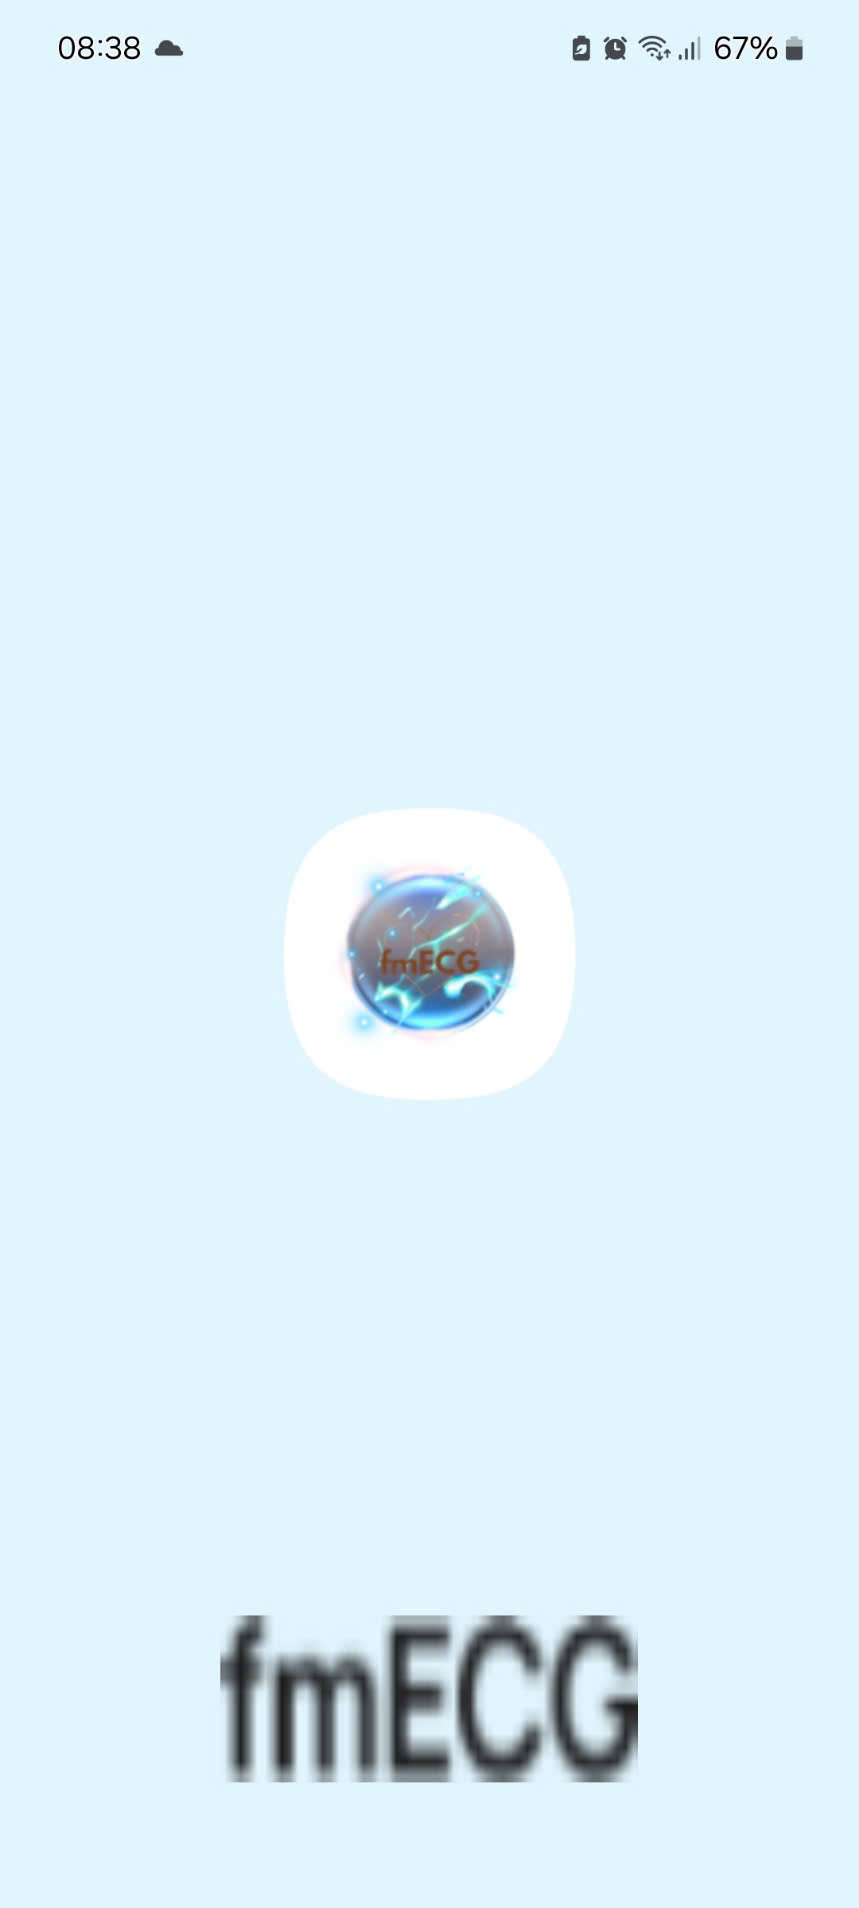
\includegraphics[width=8.5cm,height=18cm]{Images/AppUI/startApp.jpg}
	\caption[Giao diện khởi động app]{\bfseries \fontsize{12pt}{0pt}\selectfont Giao diện khởi động app}
	\label{startApp}
\end{figure}
Hình ảnh hiển thị biểu tượng chính của ứng dụng với nền màu xanh nhạt, mang lại cảm giác nhẹ nhàng và thân thiện với người dùng. Biểu tượng trung tâm là một quả cầu năng lượng với dòng chữ "fmECG," được tô điểm bằng hiệu ứng ánh sáng động, tượng trưng cho sự liên kết giữa công nghệ và y học hiện đại.

\begin{figure}[H]
	\centering
	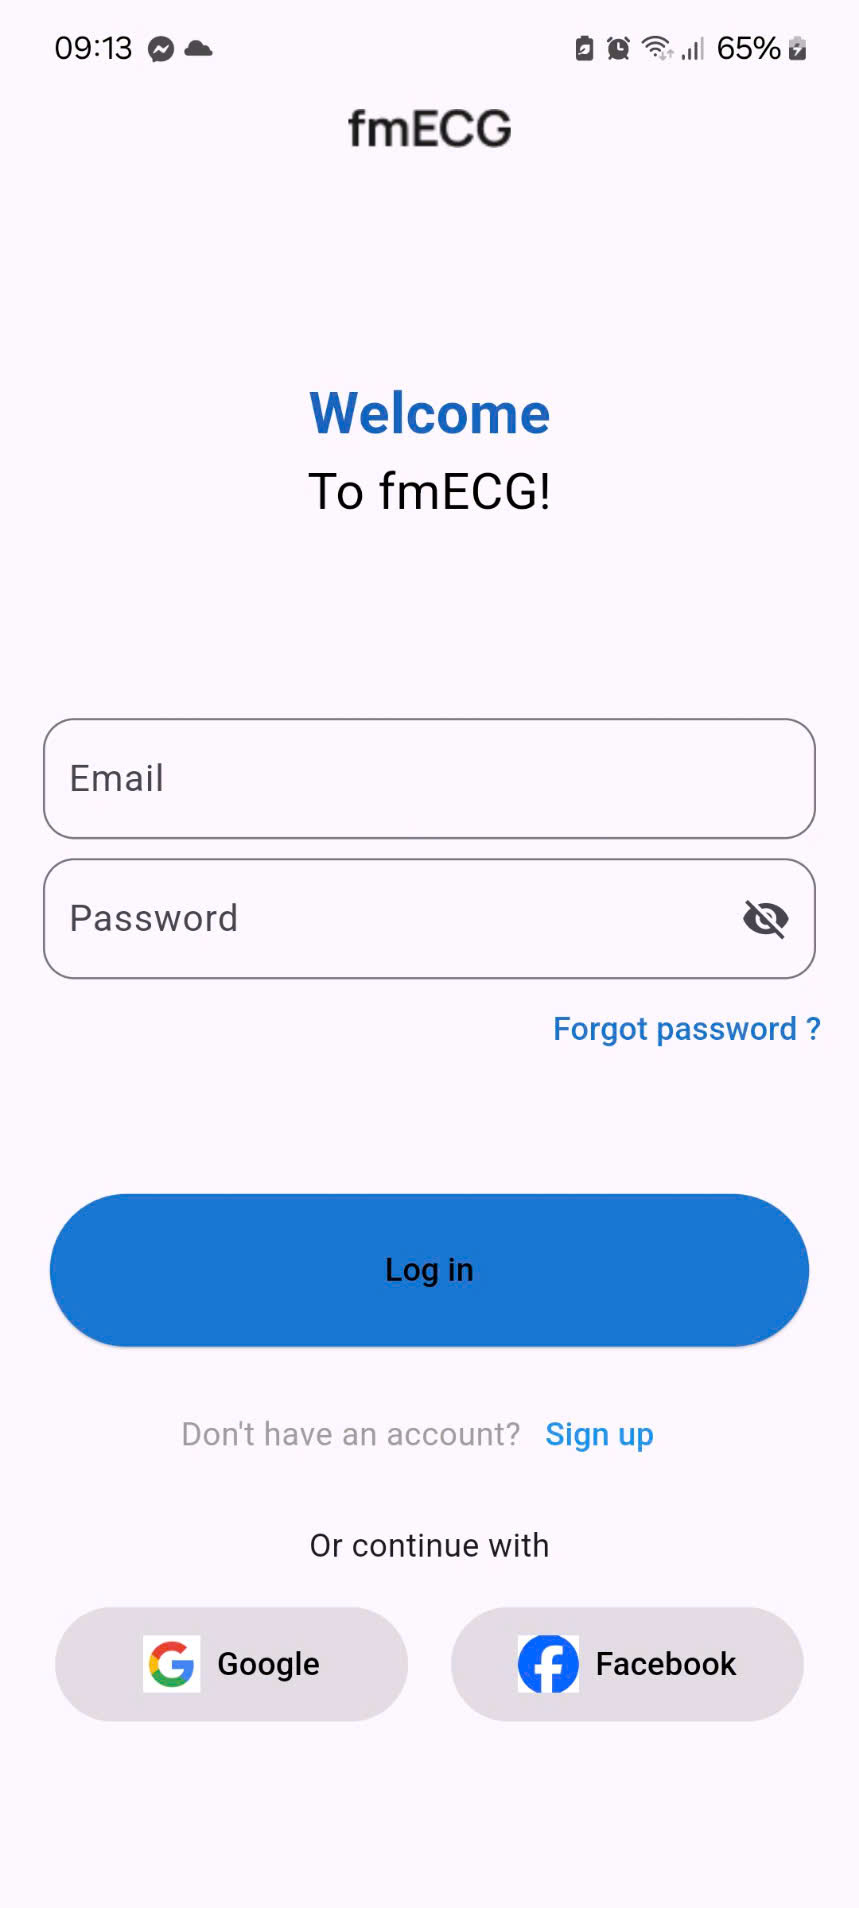
\includegraphics[width=8.5cm,height=18cm]{Images/AppUI/login.jpg}
	\caption[Giao diện trang đăng nhập]{\bfseries \fontsize{12pt}{0pt}\selectfont Giao diện trang đăng nhập}
	\label{login}
\end{figure}
Giao diện đăng nhập của ứng dụng "fmECG" được thiết kế đơn giản và thân thiện với người dùng. Ở phía trên cùng, tên ứng dụng "fmECG" được hiển thị rõ ràng, giúp người dùng dễ dàng nhận diện thương hiệu. Phía dưới là thông điệp chào mừng "Welcome to fmECG!" nhằm tạo cảm giác thân thiện và chuyên nghiệp. Giao diện cung cấp hai ô nhập thông tin: một ô dành cho "Email" và một ô cho "Password," với biểu tượng mắt đi kèm để hỗ trợ người dùng kiểm tra mật khẩu đã nhập.

\subsubsection{Giao diện của bác sĩ (Doctor)}

\begin{figure}[H]
	\centering
	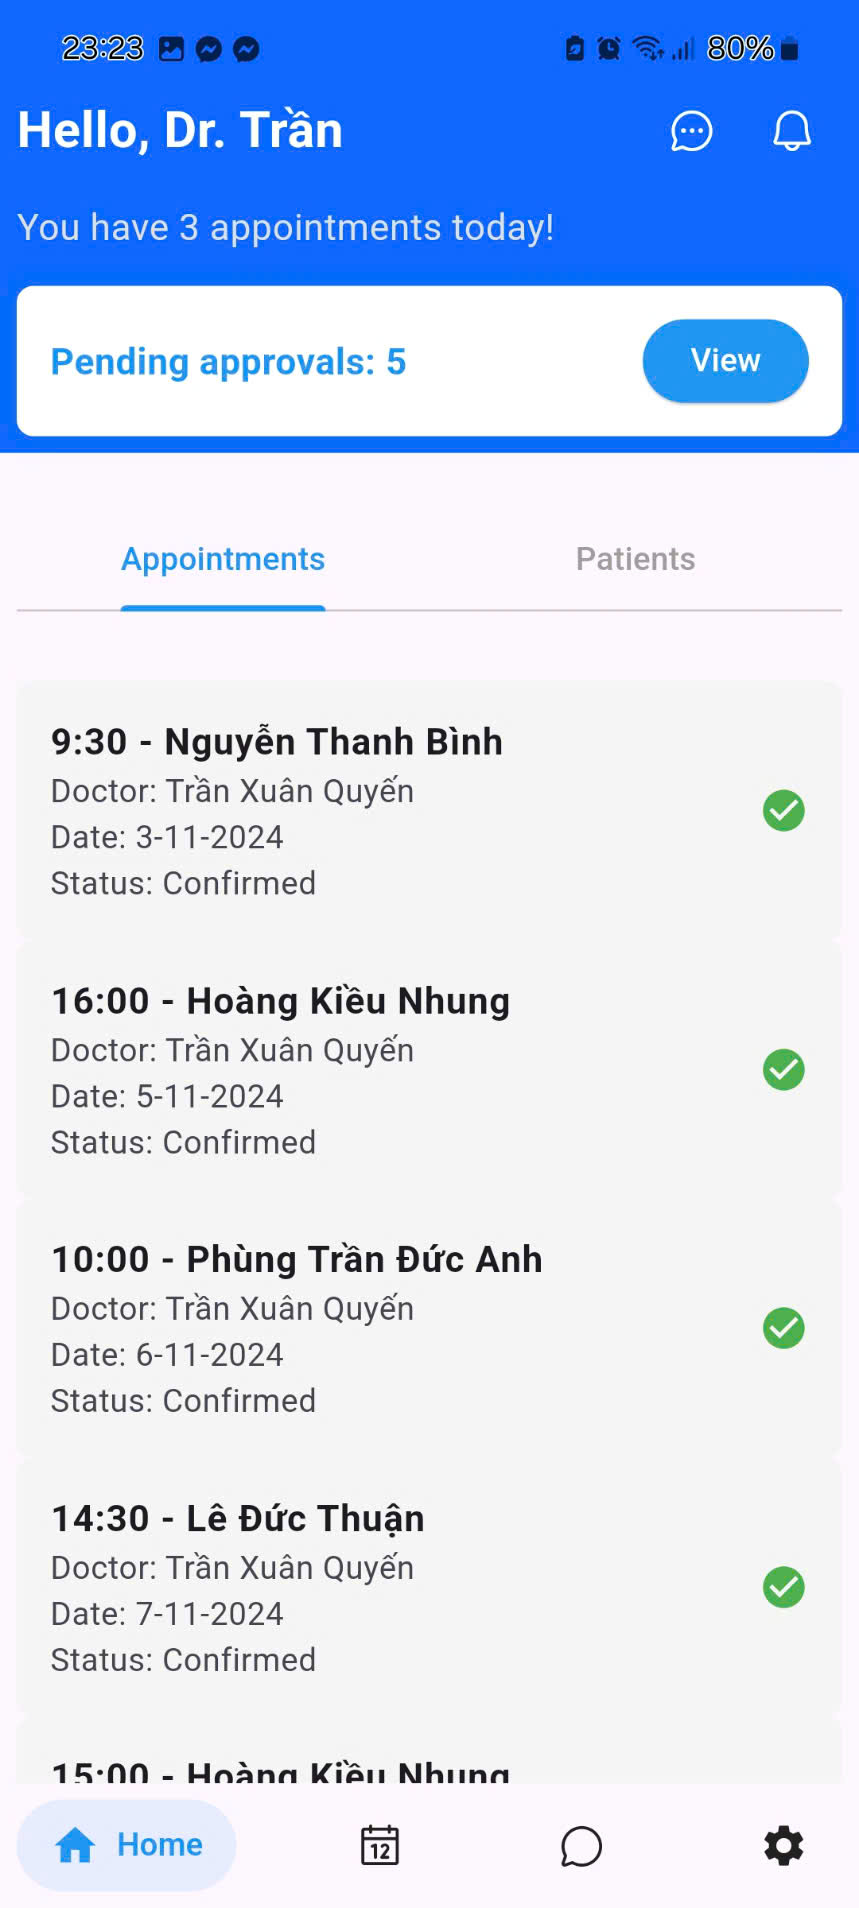
\includegraphics[width=8.5cm,height=18cm]{Images/AppUI/homePage1Doctor.jpg}
	\caption[Giao diện trang chủ của bác sĩ]{\bfseries \fontsize{12pt}{0pt}\selectfont Giao diện trang chủ của bác sĩ}
	\label{homeDoctor}
\end{figure}
Trang chủ của bác sĩ được thiết kế để cung cấp thông tin tổng quan nhanh chóng và rõ ràng. Phần trên cùng hiển thị lời chào cá nhân hóa với số lượng cuộc hẹn trong ngày, đi kèm hai biểu tượng tin nhắn và thông báo ở góc phải để bác sĩ dễ dàng theo dõi thông tin quan trọng. Ngoài ra, mục "Pending approvals" hiển thị số yêu cầu đang chờ xử lý với nút "View" để chuyển hướng đến chi tiết. Phần dưới là danh sách các cuộc hẹn đã xác nhận, bao gồm thông tin thời gian, bệnh nhân, và trạng thái.

\begin{figure}[H]
	\centering
	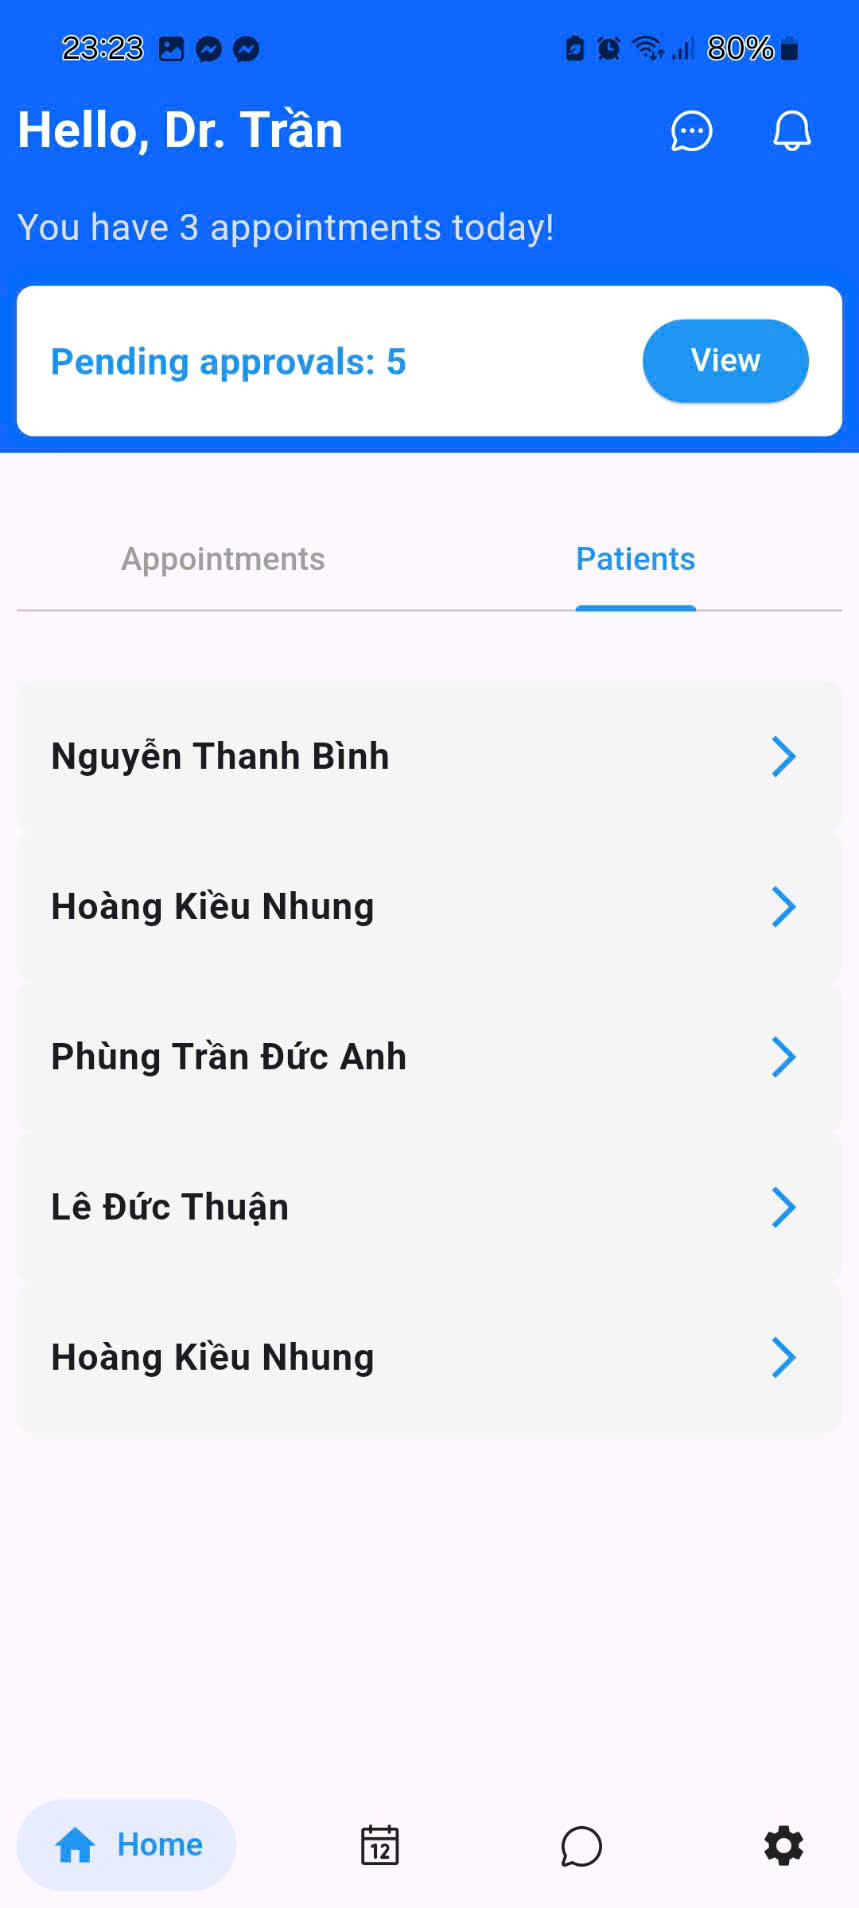
\includegraphics[width=8.5cm,height=18cm]{Images/AppUI/homePage2Doctor.jpg}
	\caption[Giao diện danh sách bệnh nhân của bác sĩ]{\bfseries \fontsize{12pt}{0pt}\selectfont Giao diện danh sách bệnh nhân của bác sĩ}
	\label{patientListDoctor}
\end{figure}
Tab "Patients" trong giao diện bác sĩ hiển thị danh sách các bệnh nhân dưới dạng các mục riêng biệt. Mỗi mục bao gồm tên bệnh nhân cùng nút điều hướng để truy cập nhanh vào hồ sơ chi tiết của từng người.

\begin{figure}[H]
	\centering
	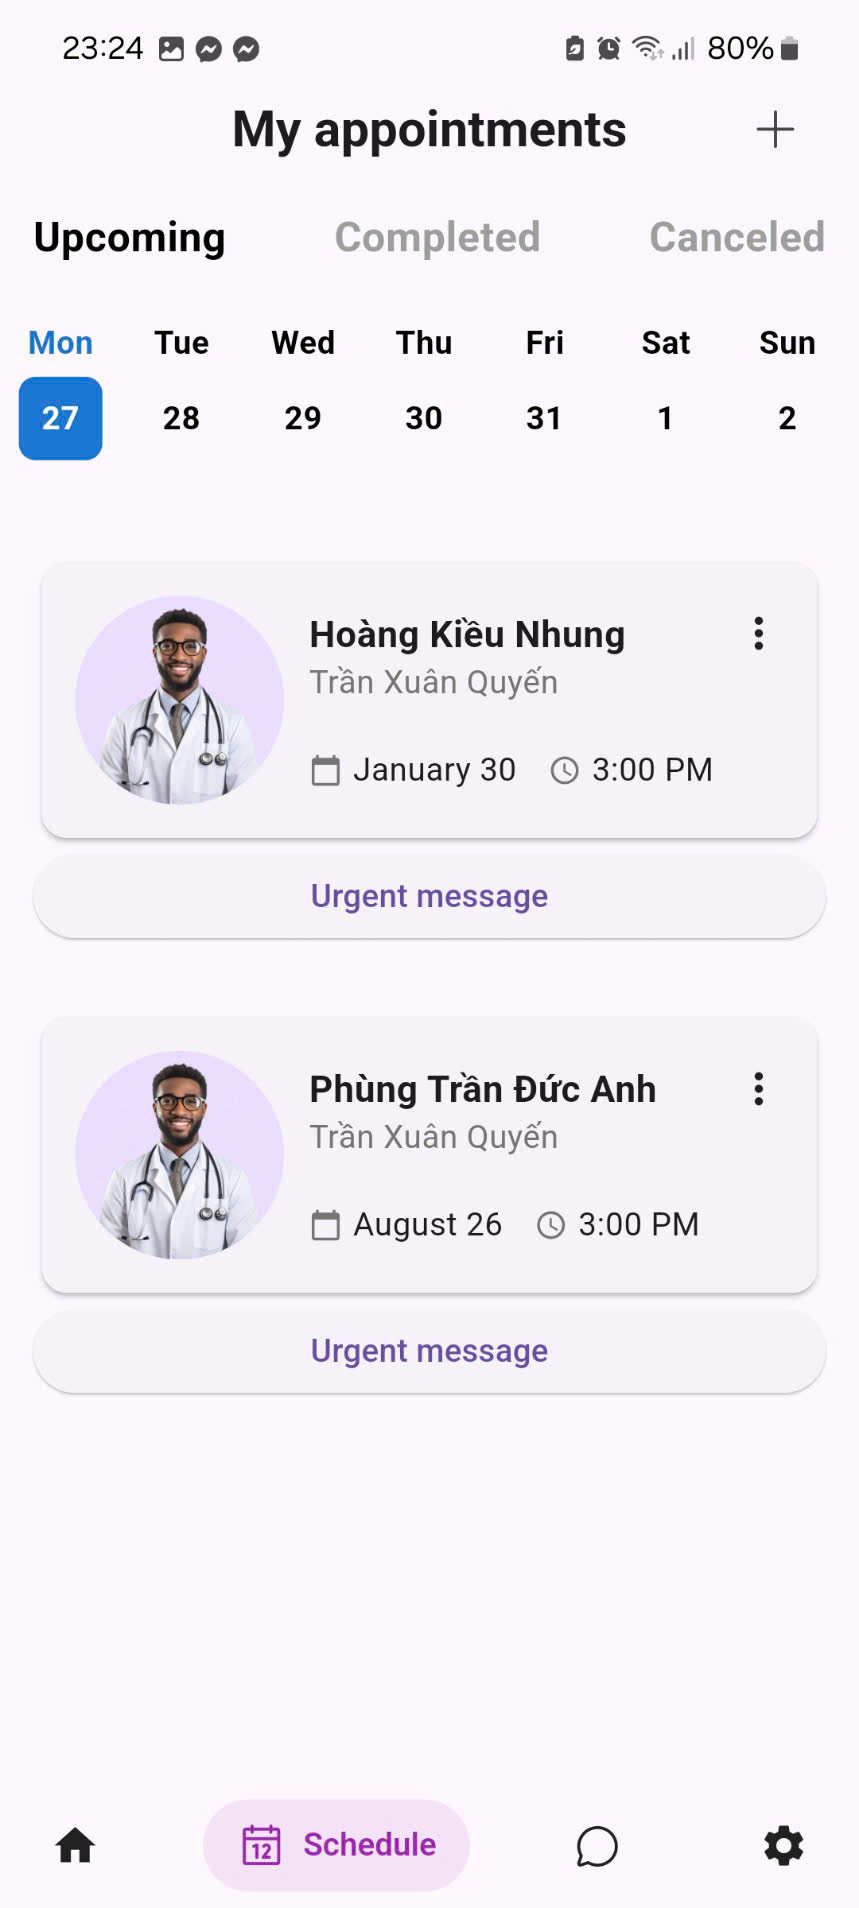
\includegraphics[width=8.5cm,height=18cm]{Images/AppUI/scheduleUpComing.jpg}
	\caption[Giao diện quản lý lịch của bác sĩ]{\bfseries \fontsize{12pt}{0pt}\selectfont Giao diện quản lý lịch của bác sĩ}
	\label{scheduleDoctor}
\end{figure}
Giao diện quản lý lịch của bác sĩ được chia thành ba tab chính: \textbf{Upcoming}, \textbf{Completed}, và \textbf{Canceled}. Tab \textbf{Upcoming} hiển thị danh sách các cuộc hẹn sắp tới với thông tin chi tiết như tên bệnh nhân, ngày và giờ hẹn, cùng nút "Urgent message" để liên lạc khẩn cấp khi cần thiết.

Sang giao diện đặt lịch:
\begin{figure}[H]
	\centering
	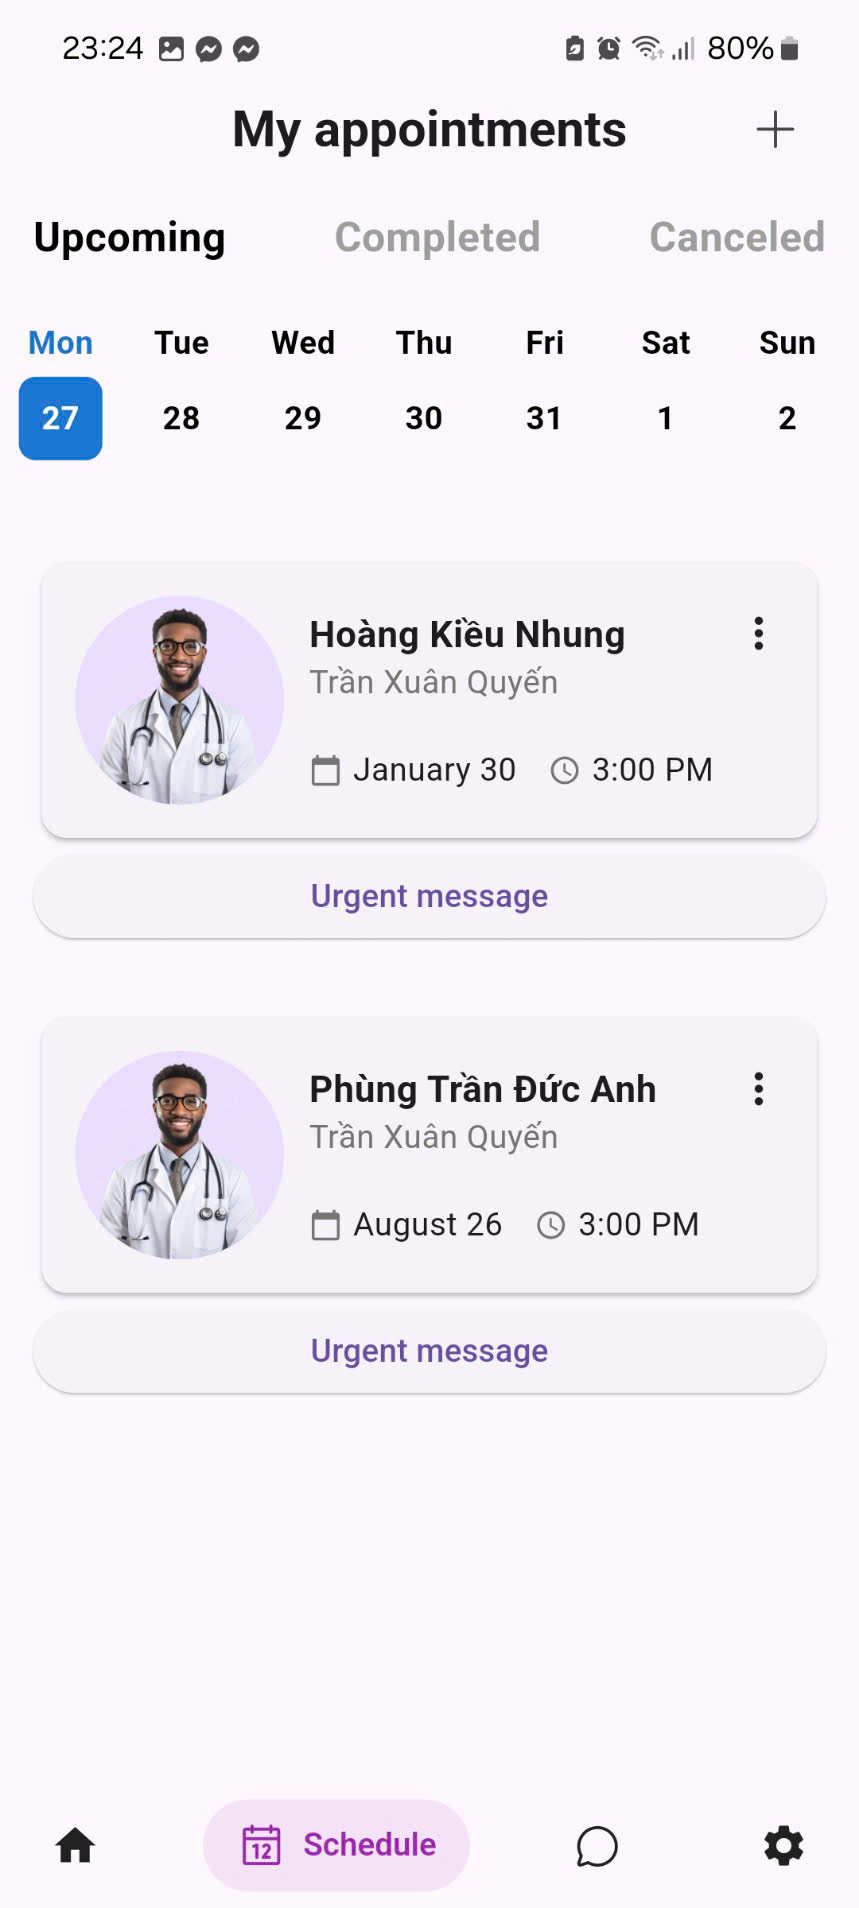
\includegraphics[width=8.5cm,height=18cm]{Images/AppUI/scheduleUpComing.jpg}
	\caption[Giao diện quản lý lịch của bác sĩ]{\bfseries \fontsize{12pt}{0pt}\selectfont Giao diện quản lý lịch của bác sĩ}
	\label{scheduleDoctor}
\end{figure}
Giao diện quản lý lịch của bác sĩ được chia thành ba tab chính: \textbf{Upcoming}, \textbf{Completed}, và \textbf{Canceled}. Tab \textbf{Upcoming} hiển thị danh sách các cuộc hẹn sắp tới với thông tin chi tiết như tên bệnh nhân, ngày và giờ hẹn, cùng nút "Urgent message" để liên lạc khẩn cấp khi cần thiết. 


\begin{figure}[H]
	\centering
	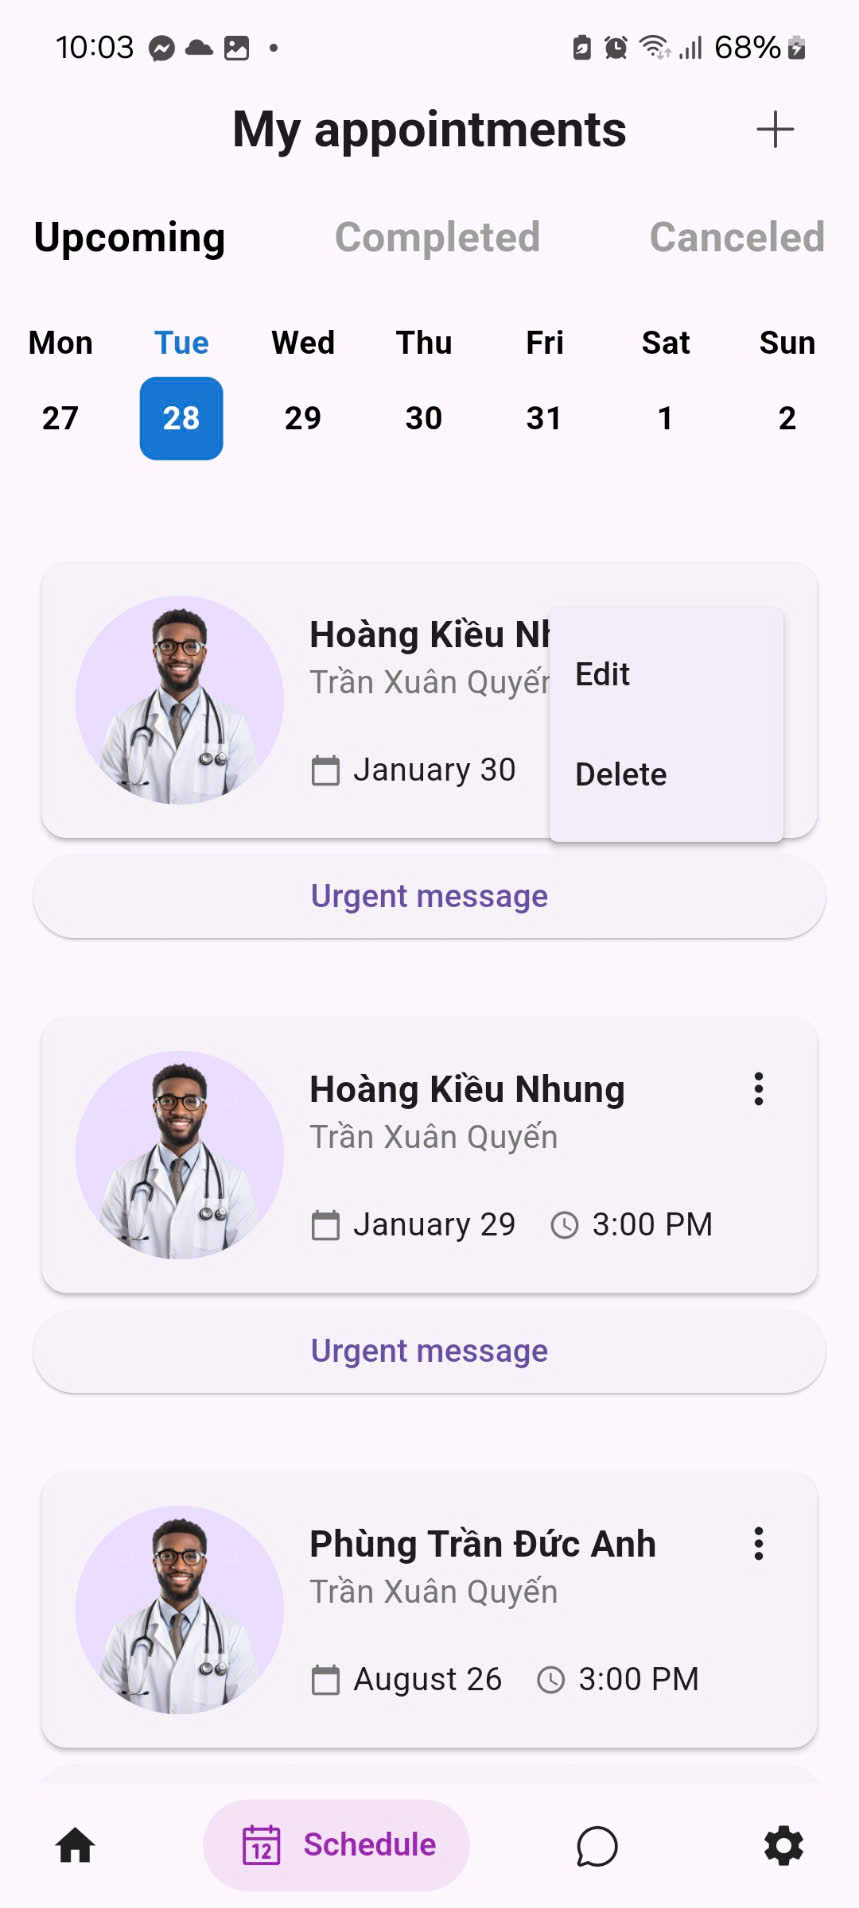
\includegraphics[width=8.5cm,height=18cm]{Images/AppUI/optionSchedule.jpg}
	\caption[Tùy chọn hủy lịch hẹn trong tab Upcoming]{\bfseries \fontsize{12pt}{0pt}\selectfont Tùy chọn hủy lịch hẹn trong tab Upcoming}
	\label{upcomingOptions}
\end{figure}
Trong tab \textbf{Upcoming}, mỗi cuộc hẹn đều có biểu tượng dấu ba chấm ở góc phải, cho phép bác sĩ truy cập vào các tùy chọn bổ sung. Một trong số đó là chức năng \textbf{Hủy lịch hẹn}. Khi nhấn vào tùy chọn này, một cửa sổ mới sẽ xuất hiện, yêu cầu bác sĩ nhập lý do hủy lịch.

\begin{figure}[H]
	\centering
	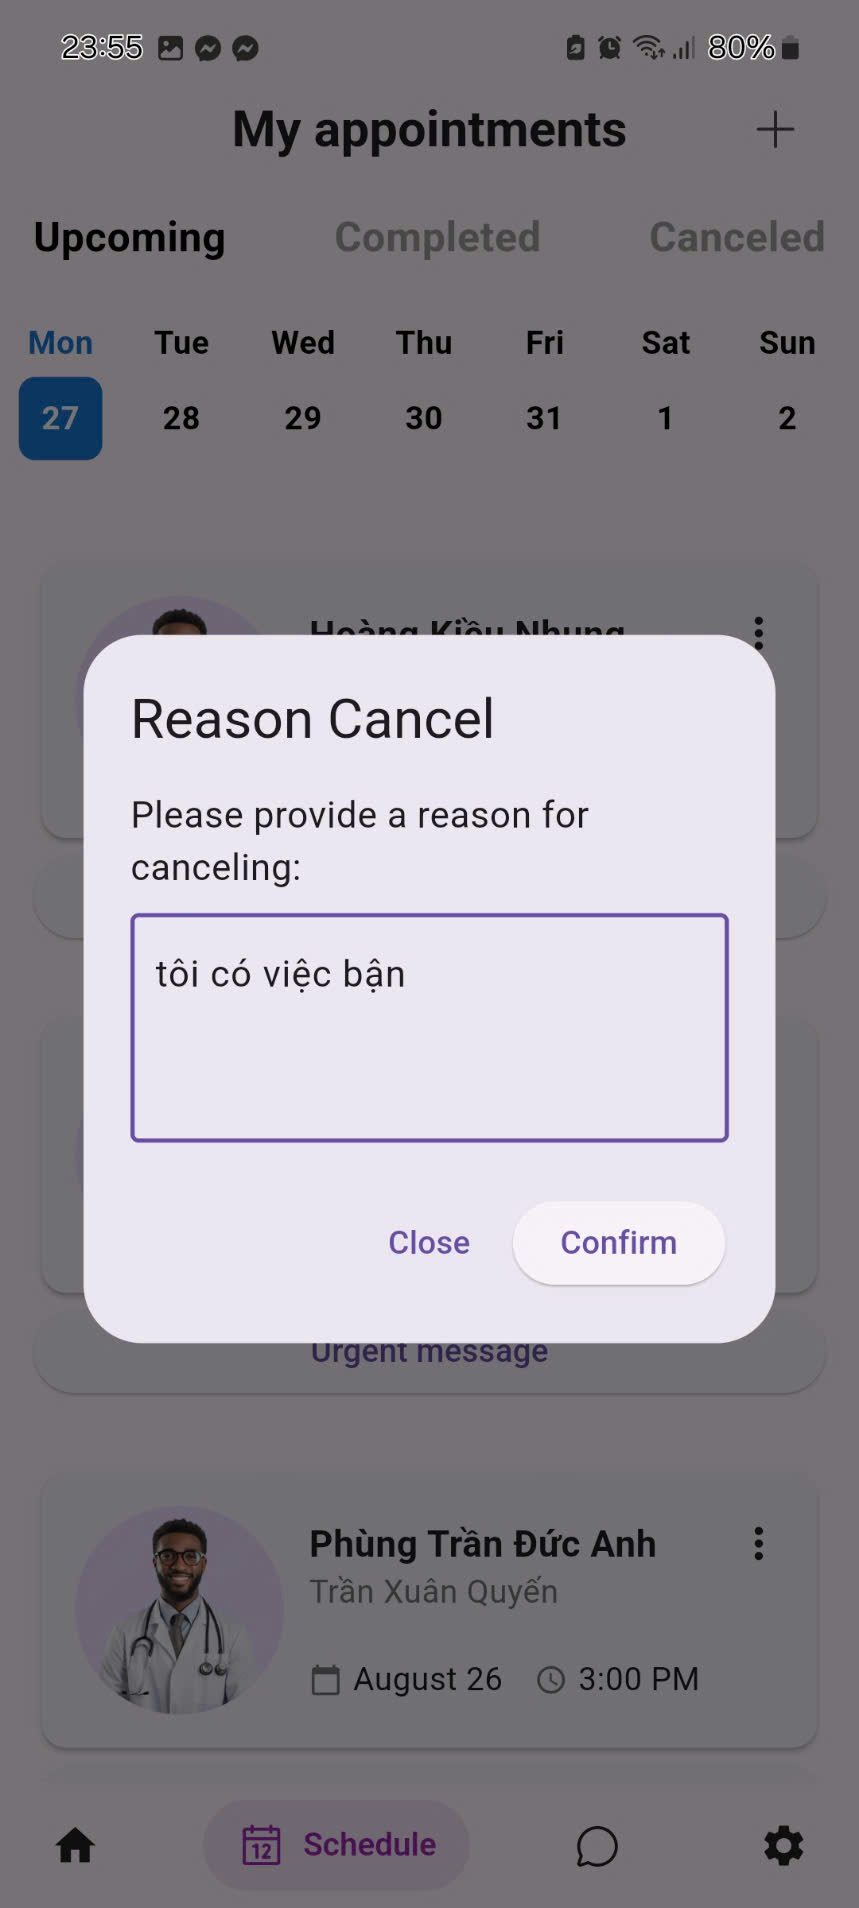
\includegraphics[width=8.5cm,height=18cm]{Images/AppUI/cancelledSchedule.jpg}
	\caption[Giao diện nhập lý do hủy lịch hẹn]{\bfseries \fontsize{12pt}{0pt}\selectfont Giao diện nhập lý do hủy lịch hẹn}
	\label{cancelAppointment}
\end{figure}
Giao diện nhập lý do hủy lịch hẹn cung cấp một ô nhập liệu để bác sĩ điền thông tin giải thích lý do hủy cuộc hẹn. Phía dưới là hai nút chức năng:
\begin{itemize}
	\item \textbf{Cancel Appointment}: Xác nhận hủy lịch hẹn sau khi lý do được nhập.
	\item \textbf{Close}: Đóng cửa sổ mà không thực hiện thay đổi.
\end{itemize}
Chức năng này đảm bảo bác sĩ có thể quản lý lịch hẹn linh hoạt, đồng thời cung cấp thông tin rõ ràng cho bệnh nhân về lý do hủy lịch.


Tab \textbf{Completed} tập hợp các cuộc hẹn đã hoàn thành. Khi nhấn vào một mục trong danh sách, bác sĩ sẽ được chuyển đến cửa sổ chi tiết, hiển thị thông tin bệnh nhân như tên, tuổi, giới tính, và số điện thoại, cùng với các tùy chọn thao tác như nhập thông tin chẩn đoán và tạo lịch tái khám. Tab \textbf{Canceled} cho phép bác sĩ theo dõi các cuộc hẹn đã bị hủy, hỗ trợ việc quản lý lịch sử làm việc dễ dàng hơn.

\begin{figure}[H]
	\centering
	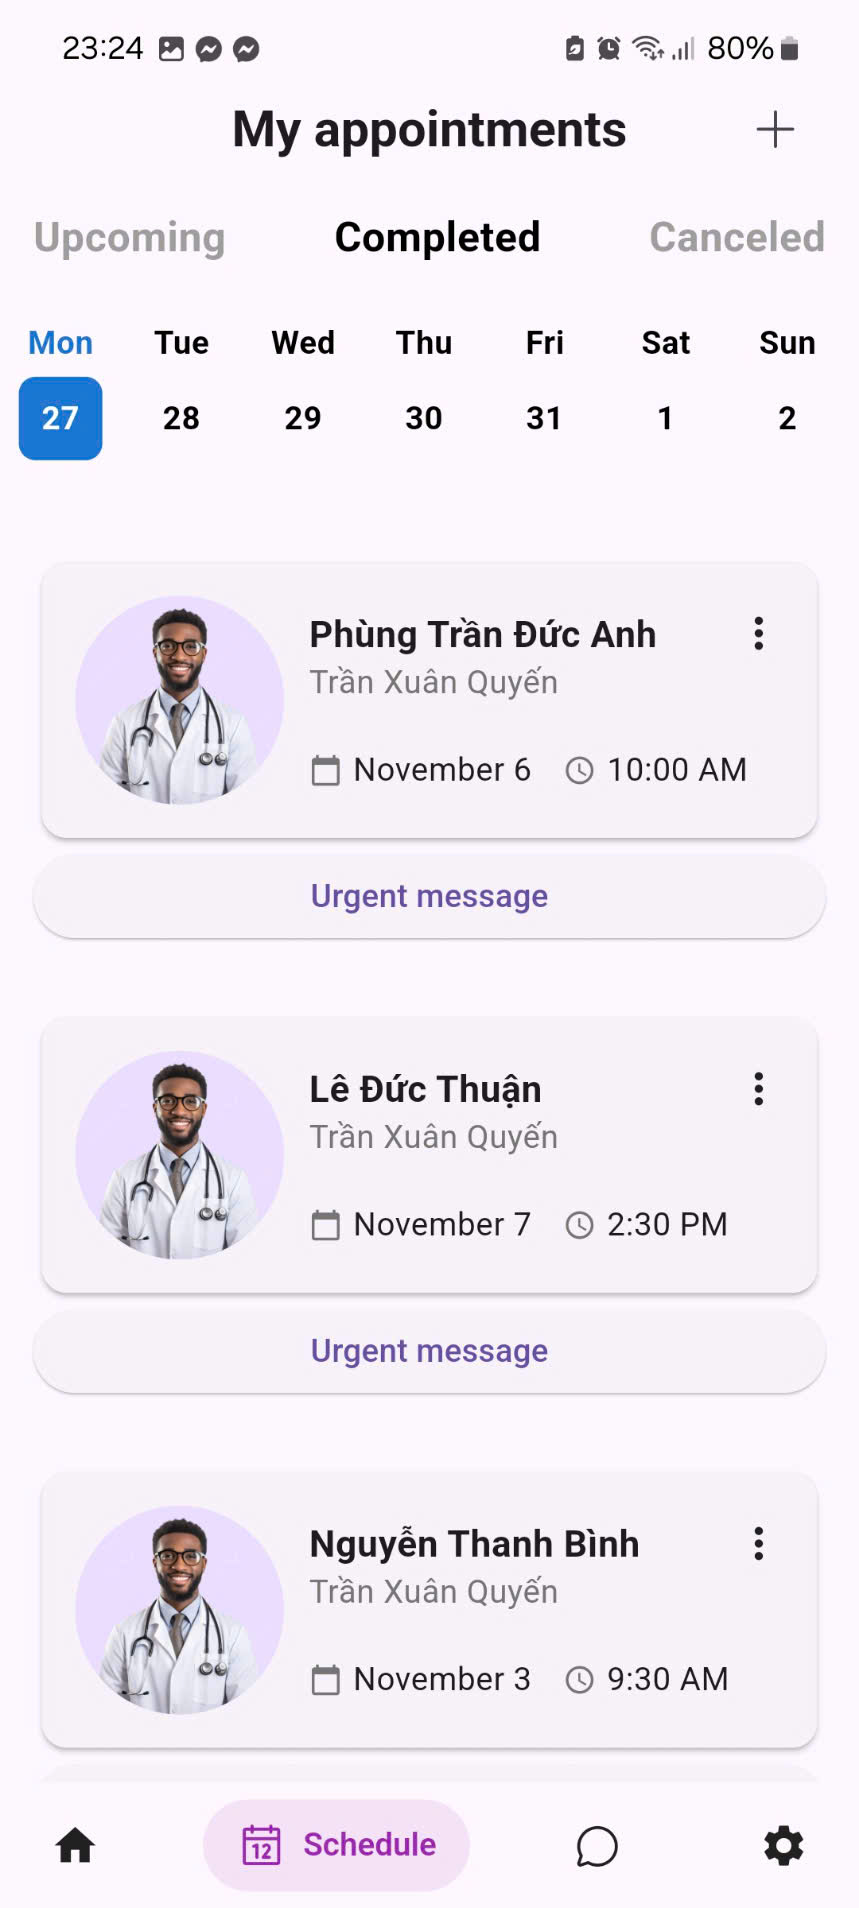
\includegraphics[width=8.5cm,height=18cm]{Images/AppUI/scheduleCompleted.jpg}
	\caption[Chi tiết thông tin bệnh nhân từ lịch đã hoàn thành]{\bfseries \fontsize{12pt}{0pt}\selectfont Chi tiết thông tin bệnh nhân từ lịch đã hoàn thành}
	\label{patientInfo}
\end{figure}
Khi truy cập vào thông tin chi tiết từ tab \textbf{Completed}, bác sĩ sẽ thấy toàn bộ thông tin về bệnh nhân, bao gồm tên, tuổi, giới tính, và số điện thoại. Bên dưới là các nút chức năng như:
\begin{itemize}
	\item \textbf{Chẩn đoán}: Cho phép bác sĩ nhập hoặc chỉnh sửa thông tin chẩn đoán cho bệnh nhân.
	\item \textbf{Tạo lịch tái khám}: Hỗ trợ bác sĩ đặt lịch tái khám mới với giao diện chọn ngày và giờ trực quan.
	\item \textbf{Đóng cửa sổ}: Kết thúc thao tác và quay lại danh sách.
\end{itemize}

\begin{figure}[H]
	\centering
	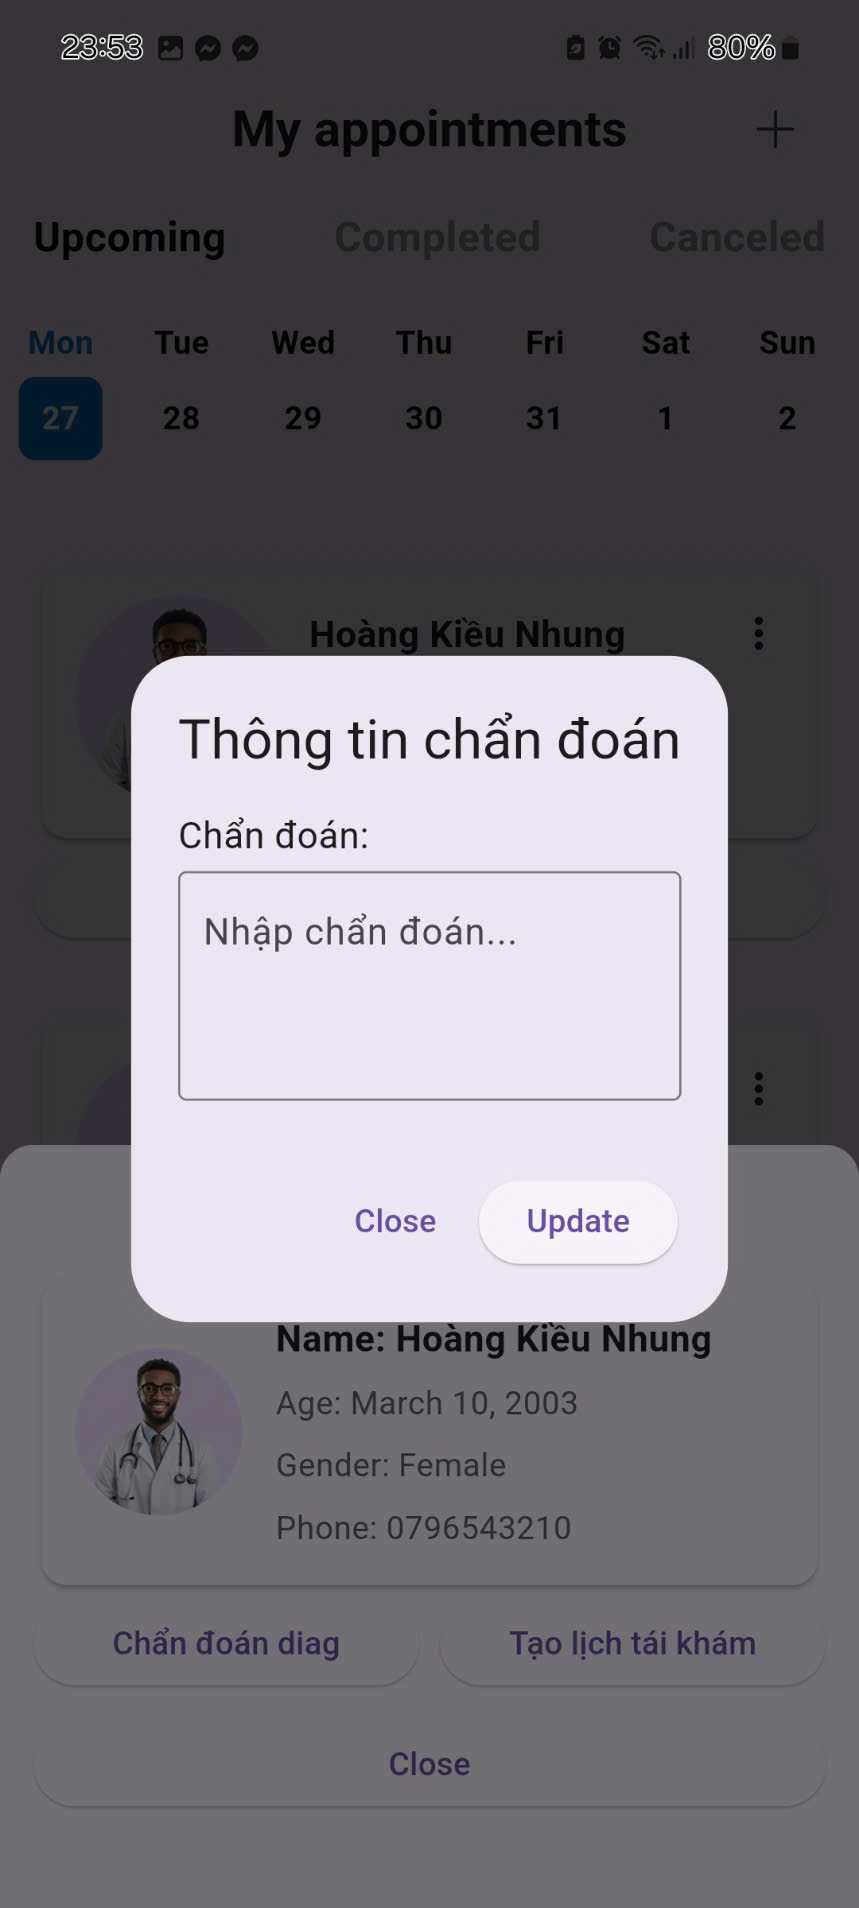
\includegraphics[width=8.5cm,height=18cm]{Images/AppUI/blockInputDIag.jpg}
	\caption[Cửa sổ cập nhật thông tin chẩn đoán]{\bfseries \fontsize{12pt}{0pt}\selectfont Cửa sổ cập nhật thông tin chẩn đoán}
	\label{diagnosisUpdate}
\end{figure}
Giao diện cập nhật chẩn đoán cung cấp một ô nhập liệu để bác sĩ thêm hoặc chỉnh sửa nội dung chẩn đoán, đi kèm nút \textbf{Update} để lưu thông tin mới.

\begin{figure}[H]
	\centering
	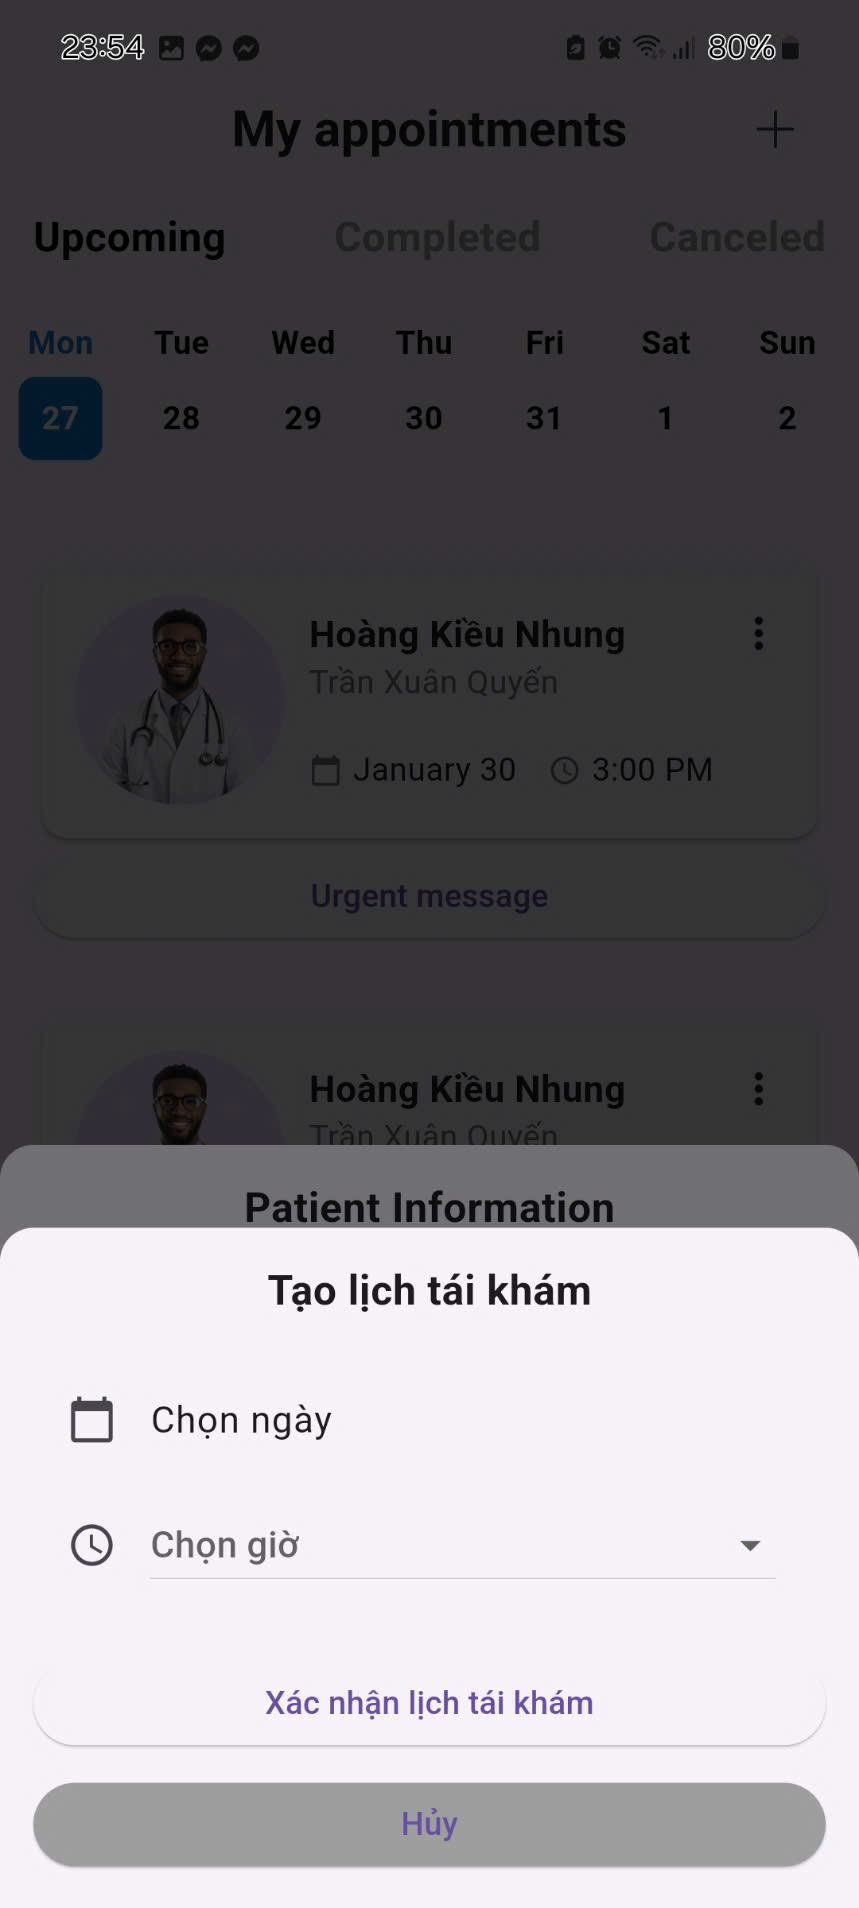
\includegraphics[width=8.5cm,height=18cm]{Images/AppUI/repickSchedule2.jpg}
	\caption[Cửa sổ tạo lịch tái khám]{\bfseries \fontsize{12pt}{0pt}\selectfont Cửa sổ tạo lịch tái khám}
	\label{reschedule}
\end{figure}
Giao diện đặt lịch tái khám cho phép bác sĩ chọn ngày và giờ, sau đó xác nhận bằng nút \textbf{Xác nhận lịch tái khám}. Điều này giúp đảm bảo việc quản lý các cuộc hẹn diễn ra mượt mà và hiệu quả.

\begin{figure}[H]
	\centering
	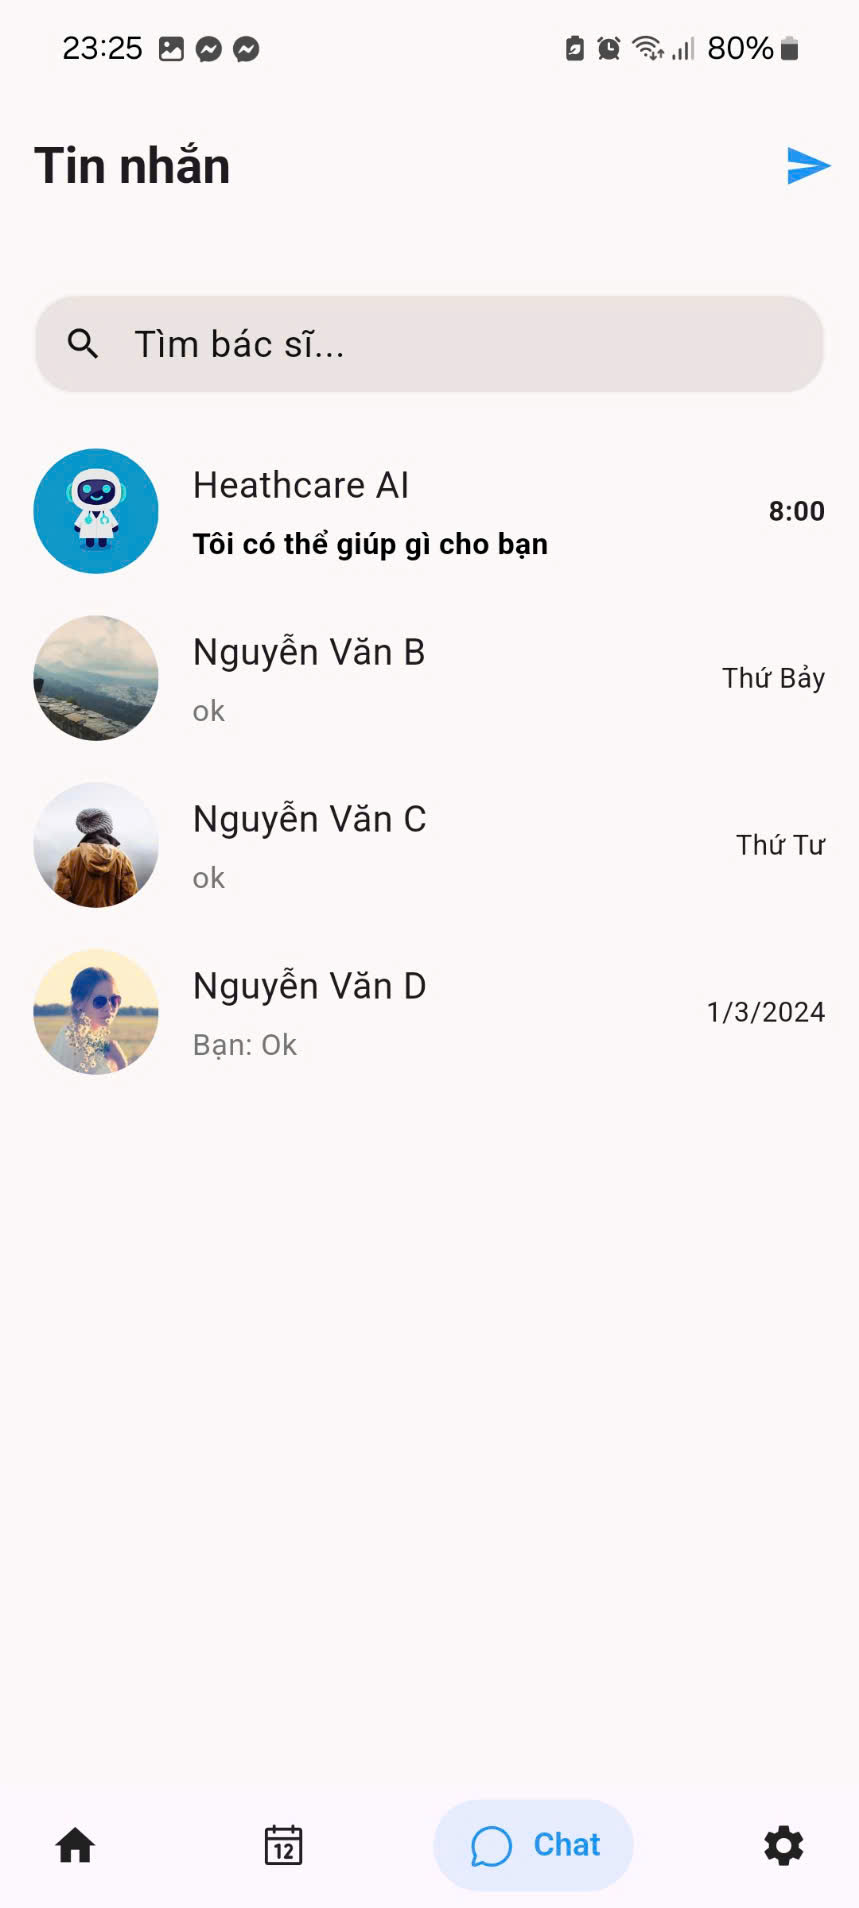
\includegraphics[width=8.5cm,height=18cm]{Images/AppUI/chatDoctor.jpg}
	\caption[Giao diện trang hội thoại]{\bfseries \fontsize{12pt}{0pt}\selectfont Giao diện trang hội thoại}
	\label{chat}
\end{figure}
Giao diện trên thuộc màn hình của bác sĩ, được thiết kế để tạo cuộc hội thoại giữa bác sĩ và bệnh nhân. Tại đây, bác sĩ có thể dễ dàng tìm kiếm tên bệnh nhân hoặc truy cập nhanh các cuộc hội thoại thông qua danh sách hiển thị ở giữa màn hình. Mỗi cuộc hội thoại đều đi kèm với tên người liên hệ, tin nhắn gần nhất, và thời gian trao đổi, giúp bác sĩ nhanh chóng xác định nội dung cần trao đổi.

\begin{figure}[H]
	\centering
	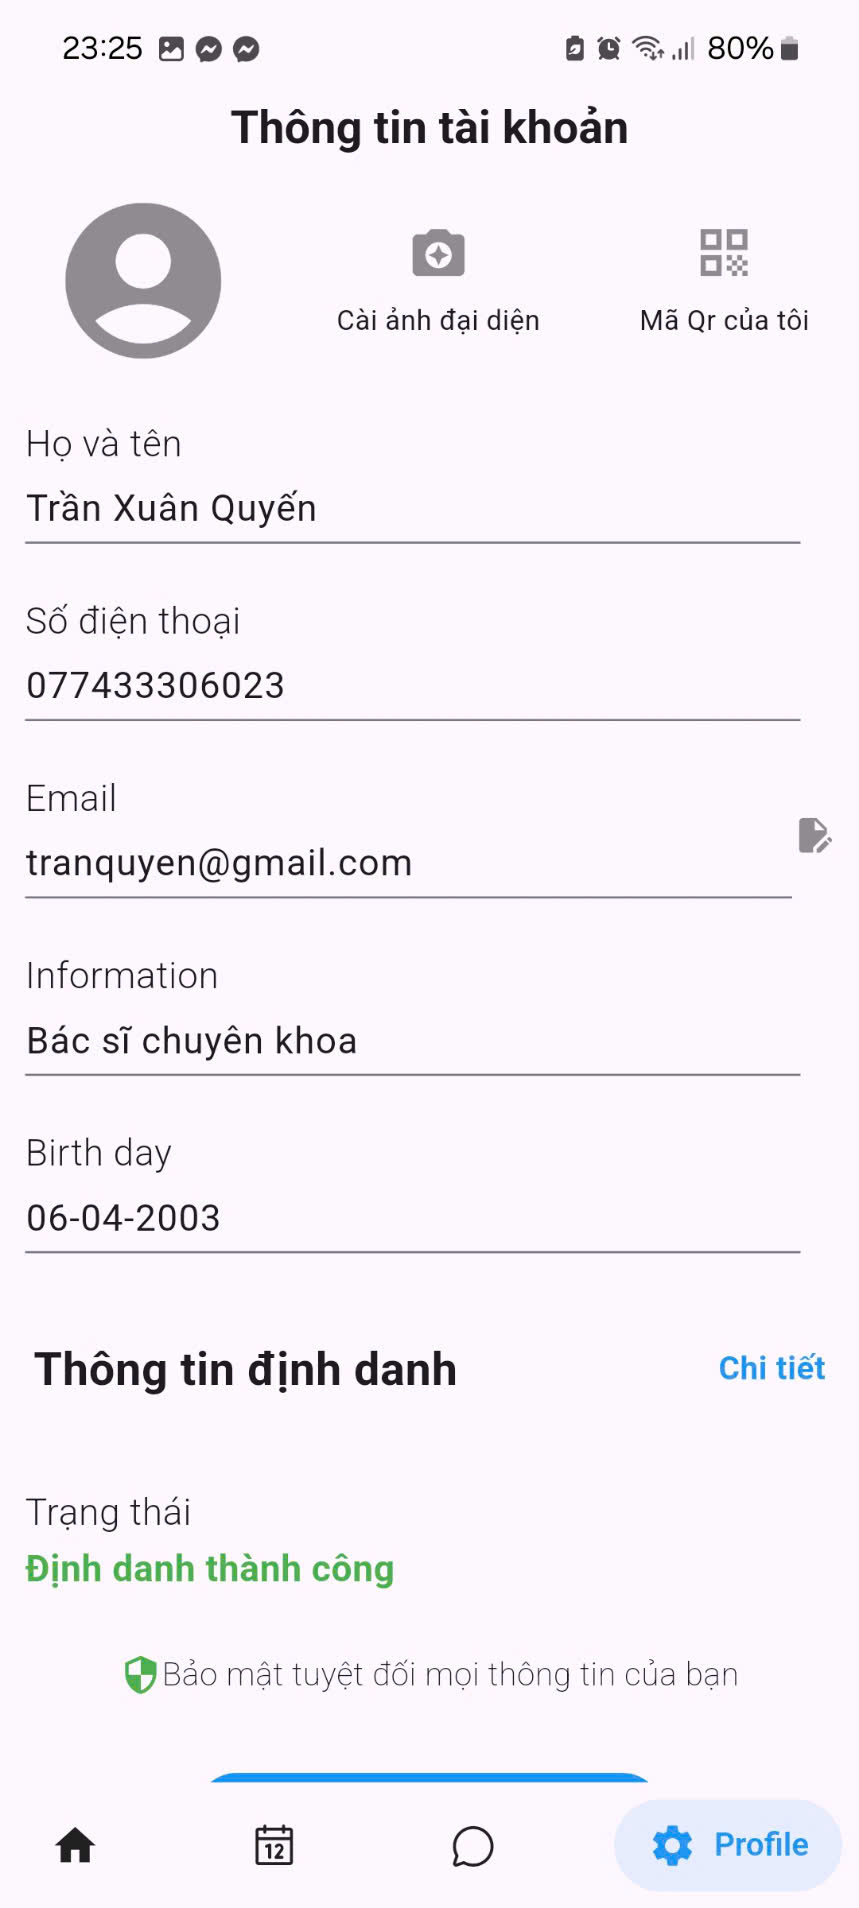
\includegraphics[width=8.5cm,height=18cm]{Images/AppUI/infoDoctor.jpg}
	\caption[Giao diện màn thông tin của bác sĩ]{\bfseries \fontsize{12pt}{0pt}\selectfont Giao diện màn thông tin của bác sĩ}
	\label{infoDoctor}
\end{figure}

Trong phần "Profile" dành cho bác sĩ, giao diện cung cấp đầy đủ các chi tiết cơ bản như họ và tên, số điện thoại, email, và ngày sinh của người dùng. Ngoài ra, chức năng hiển thị rõ vai trò chuyên môn của bác sĩ, chẳng hạn như "Bác sĩ chuyên khoa". Một điểm nổi bật là tính năng định danh tài khoản, được hiển thị với trạng thái "Định danh thành công", nhằm đảm bảo bảo mật và xác thực thông tin của bác sĩ. Giao diện trực quan, dễ sử dụng, giúp bác sĩ nhanh chóng truy cập và cập nhật thông tin cá nhân.


\begin{figure}[H]
	\centering
	
\includegraphics[width=8.5cm,height=6cm]{Images/AppUI/buttonInfoPage.png}
	\caption[Giao diện màn thông tin của bác sĩ]{\bfseries \fontsize{12pt}{0pt}\selectfont Giao diện màn thông tin của bác sĩ}
	\label{infoDoctor}
\end{figure}

Ngoài việc cung cấp các thông tin cá nhân chi tiết, phần này còn có hai nút chức năng quan trọng: "Cập nhật lại định danh" và "Đăng xuất". Nút "Cập nhật lại định danh" cho phép bác sĩ xác thực lại thông tin tài khoản để đảm bảo tính chính xác và an toàn. Trong khi đó, nút "Đăng xuất" được thiết kế với màu đỏ nổi bật, giúp bác sĩ nhanh chóng thoát khỏi tài khoản khi cần thiết. Cả hai nút đều được đặt ở vị trí dễ thấy, hỗ trợ tốt cho việc quản lý tài khoản một cách hiệu quả.
\subsubsection{Giao diện của bệnh nhân (Patient)}

\begin{figure}[H]
	\centering
	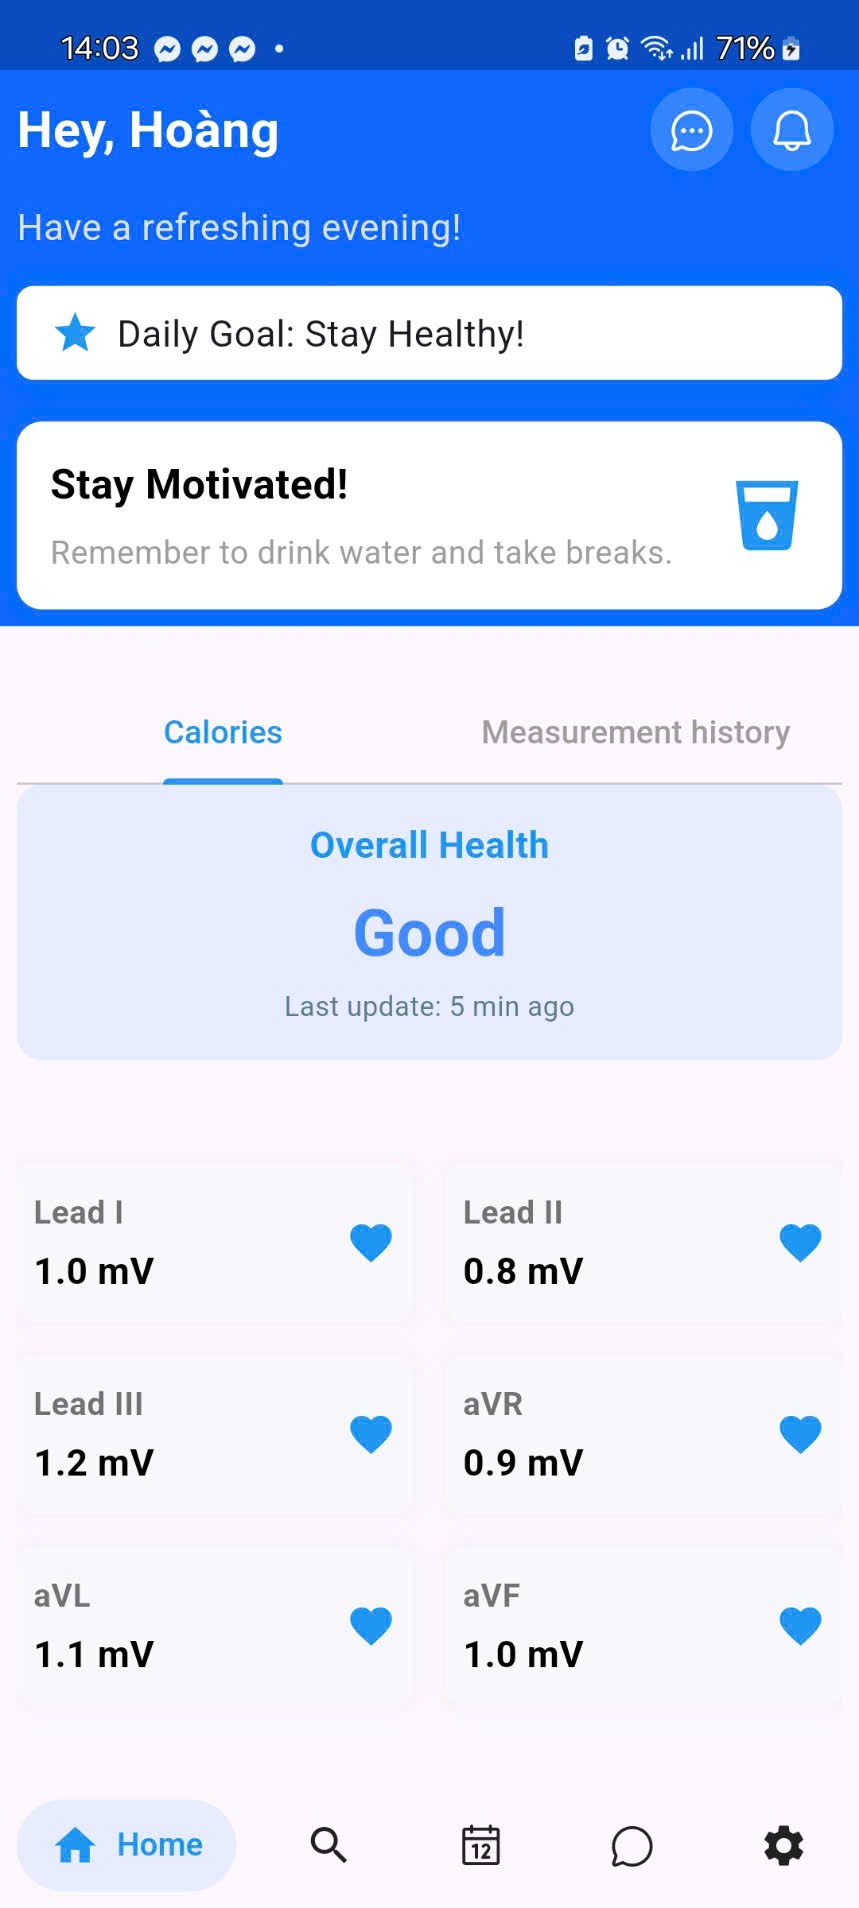
\includegraphics[width=8.5cm,height=18cm]{Images/AppUI/homePagePatient.jpg}
	\caption[Giao diện thông tin sức khỏe của bệnh nhân]{\bfseries \fontsize{12pt}{0pt}\selectfont Giao diện thông tin sức khỏe của bệnh nhân}
	\label{healthInfoPatient}
\end{figure}
Giao diện của bệnh nhân tập trung vào việc hiển thị trạng thái sức khỏe tổng quan với đánh giá "Overall Health: Good" được cập nhật gần nhất. Bên dưới là 6 số liệu liên quan đến điện tim, được trình bày rõ ràng và dễ hiểu. Những số liệu này giúp bệnh nhân theo dõi tình trạng sức khỏe tim mạch của mình một cách trực quan và chi tiết.


\begin{figure}[H]
	\centering
	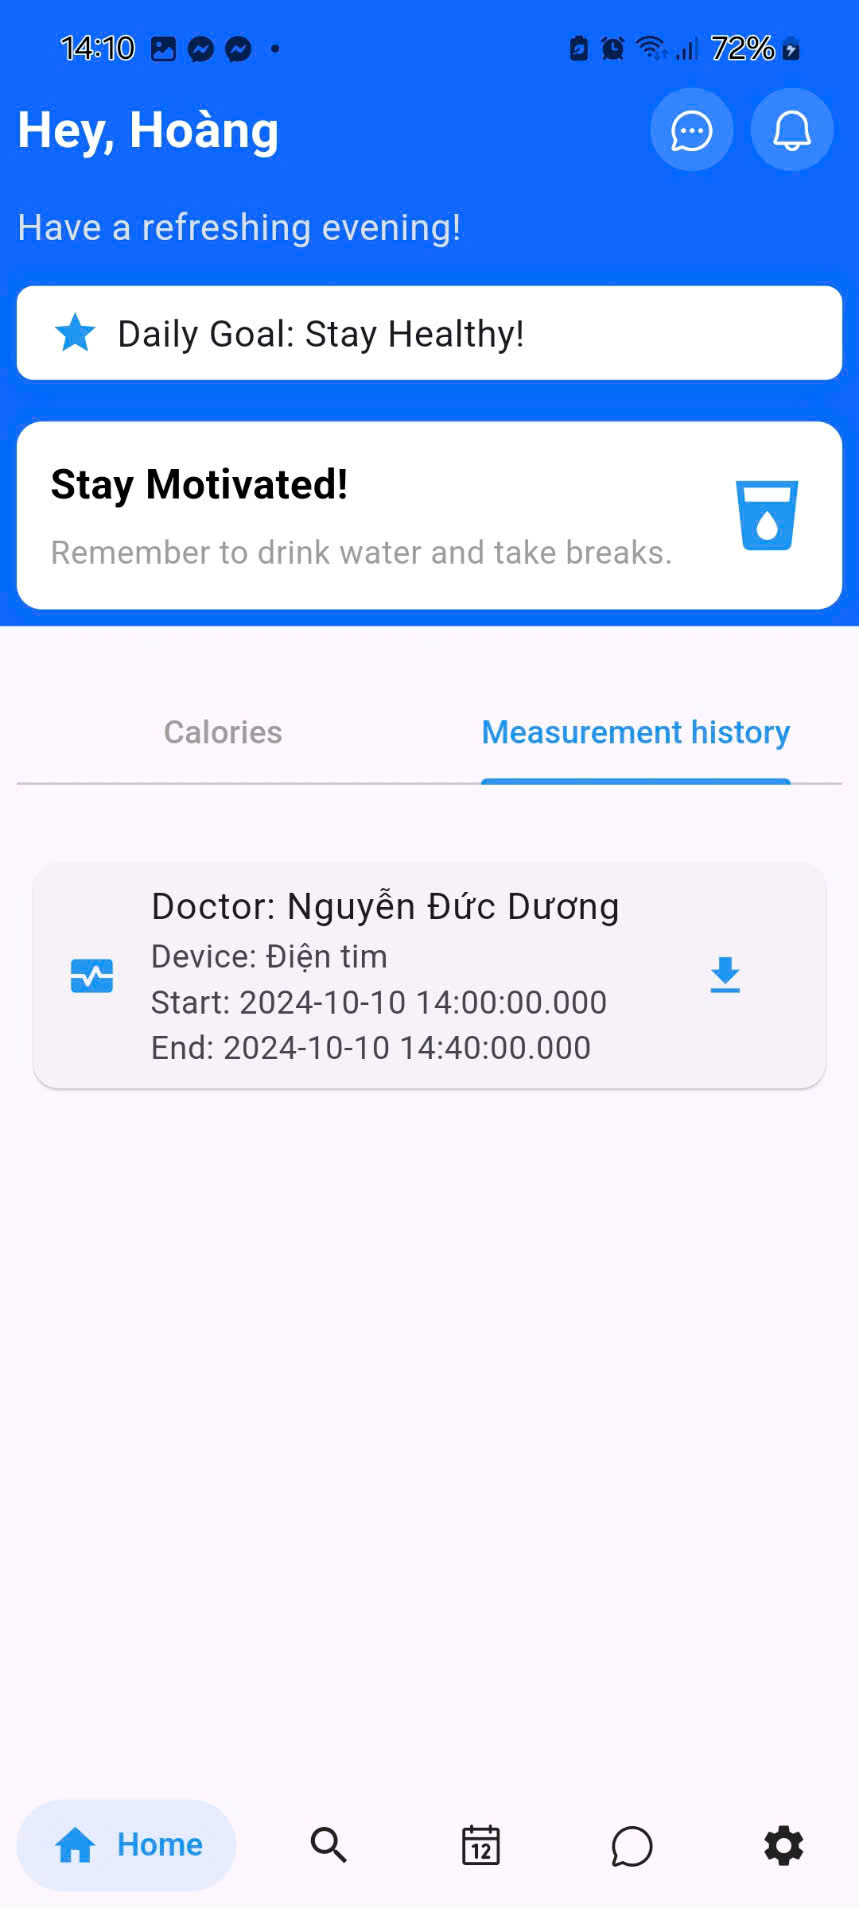
\includegraphics[width=8.5cm,height=18cm]{Images/AppUI/homePagePatient2.jpg}
	\caption[Giao diện lịch sử đo của bệnh nhân]{\bfseries \fontsize{12pt}{0pt}\selectfont Giao diện lịch sử đo của bệnh nhân}
	\label{measurementHistory}
\end{figure}
	Ở Tab \textbf{Measurement history}, cung cấp cho bệnh nhân lịch sử các lần đo trước đo với tên bác sĩ cùng với đó là thời gian bắt đầu đo và thời gian kết thúc đo, tên thiết bị đo.

\begin{figure}[H]
		\centering
		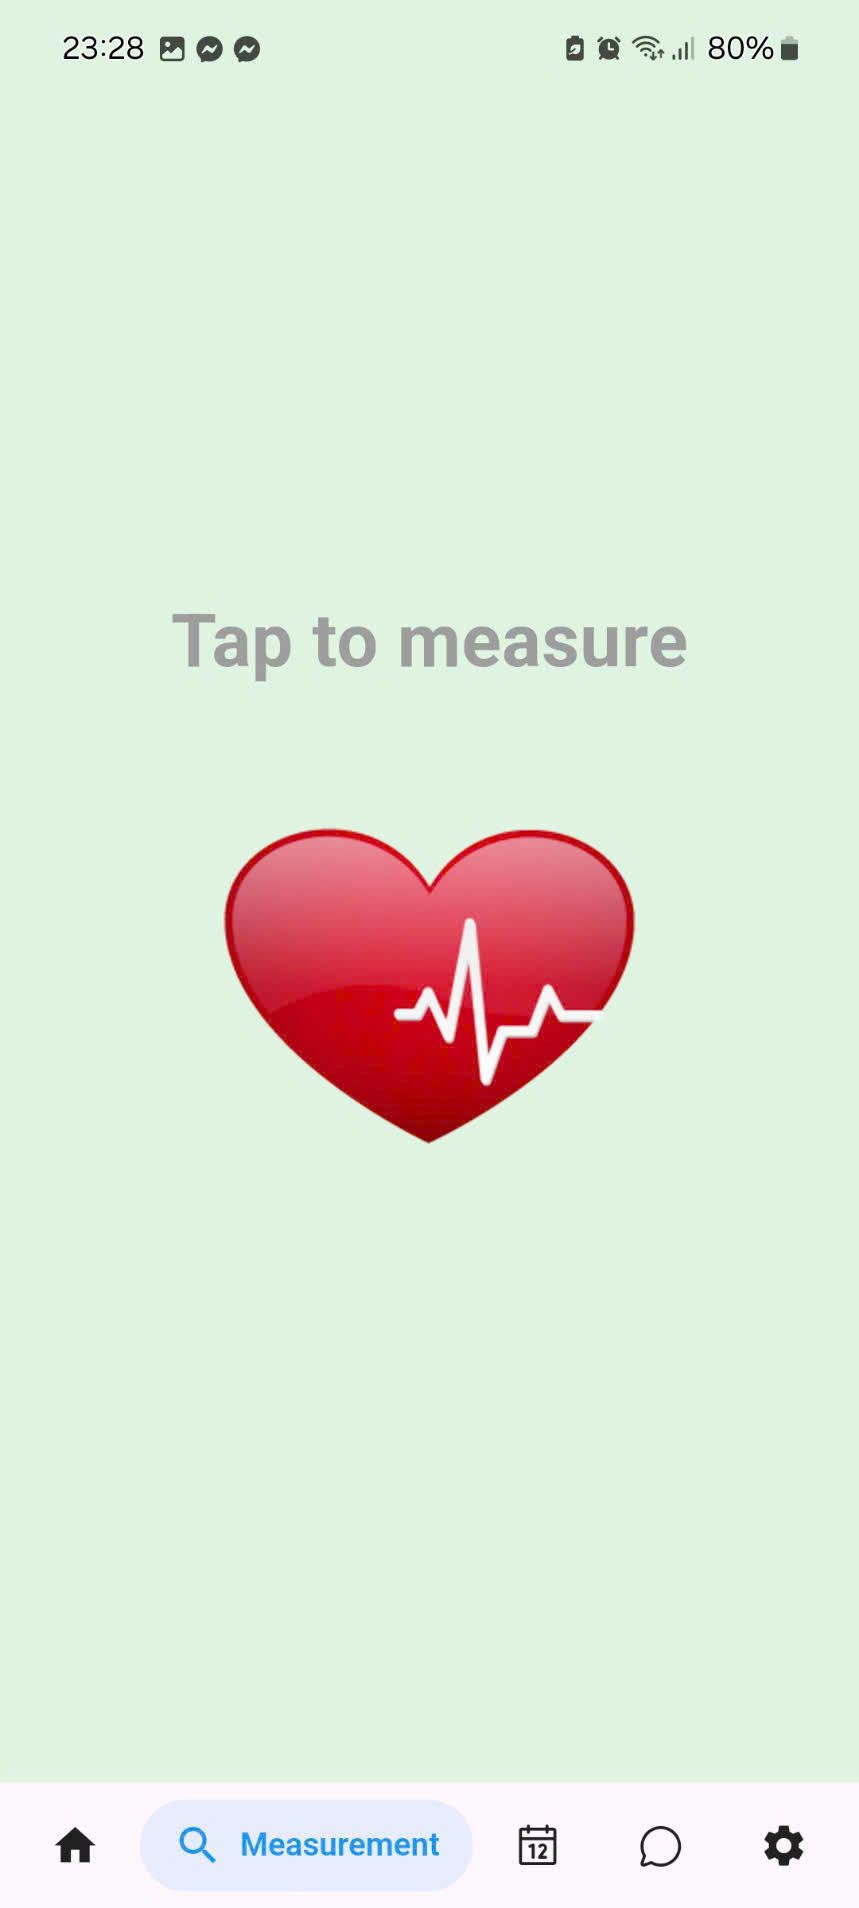
\includegraphics[width=8.5cm,height=18cm]{Images/AppUI/measure.jpg}
		\caption[Giao diện đo tín hiệu điện tim của bệnh nhân]{\bfseries \fontsize{12pt}{0pt}\selectfont Giao diện đo tin hiệu điện tim của bệnh nhân}
		\label{measurement}
\end{figure}
	Đây là giao diện phần Measurement khi bệnh nhân muốn đo tín hiệu điện tim, khi click vào hình trái tim, thiết bị sẽ bắt đầu đo và kết quả sẽ được hiển thị trên màn hình điện thoại của bệnh nhân.

	Giao diện phần đặt lịch Schedules, chủ yếu vẫn khá giống giao diện bên phần của bác sĩ, có sự khác biệt khi click vào nút "+" ở bên trên góc phải, sẽ xuất hiện màn hình lựa chọn
\begin{figure}[H]
		\centering
		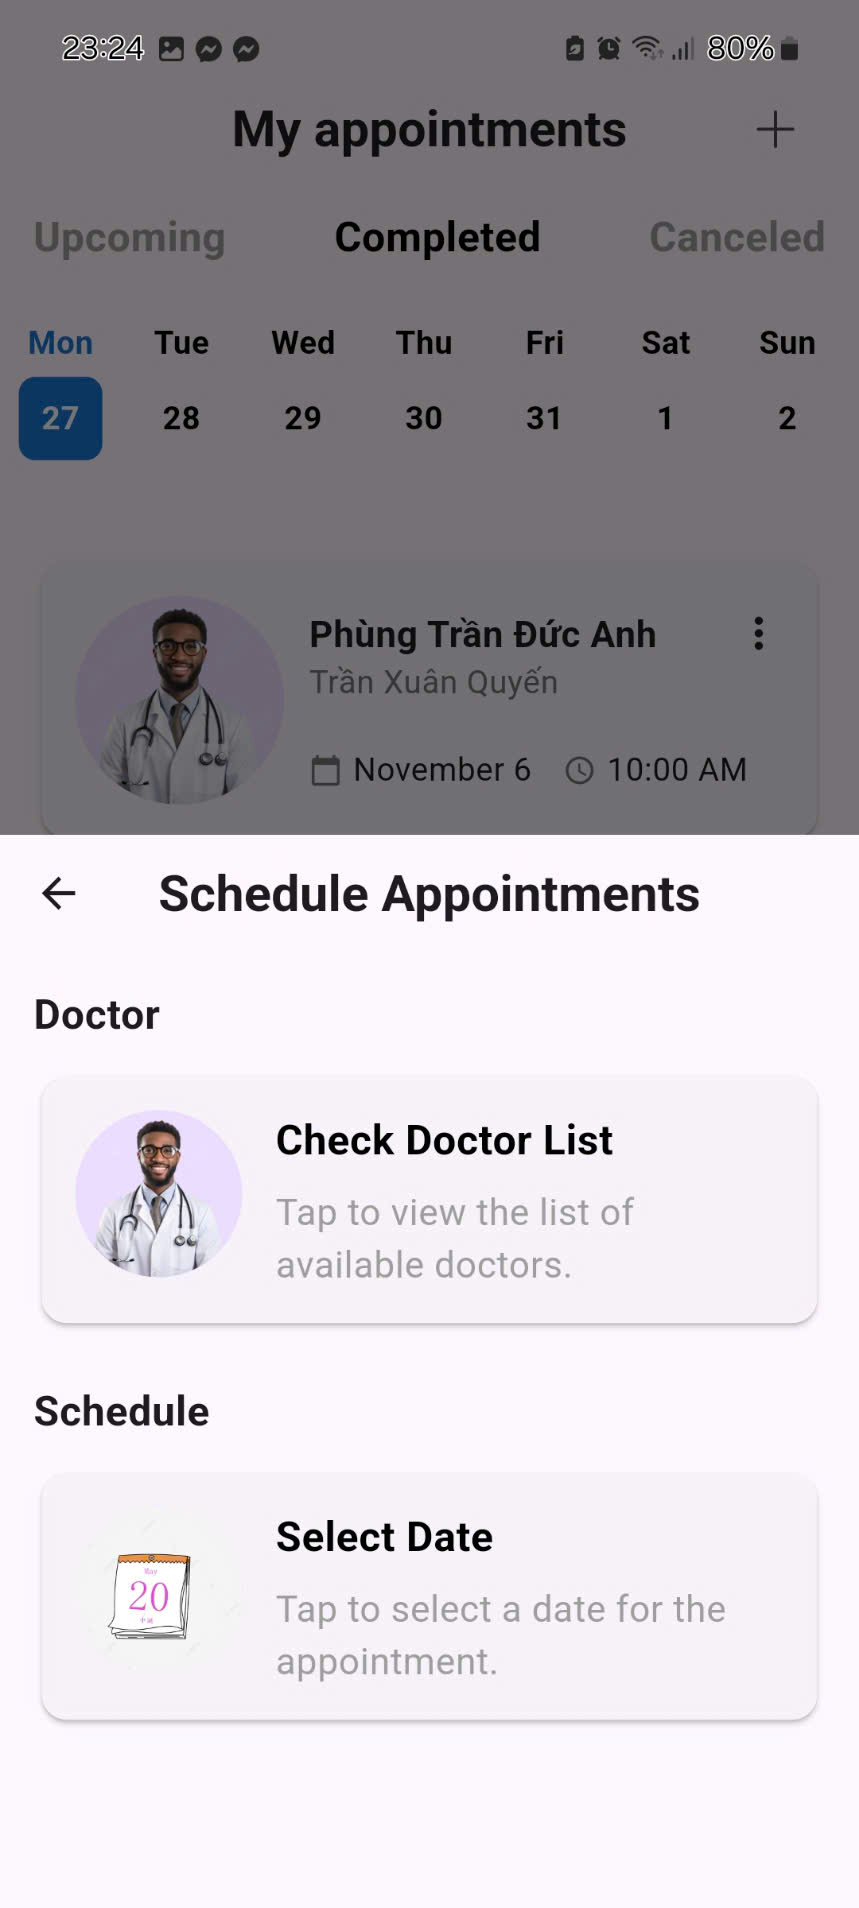
\includegraphics[width=8.5cm,height=18cm]{Images/AppUI/scheduleChoice.jpg}
		\caption[Giao diện lựa chọn kiểu đặt lịch cho bệnh nhân]{\bfseries \fontsize{12pt}{0pt}\selectfont Giao diện lựa chọn kiểu đặt lịch của bệnh nhân}
		\label{scheduleChoice}
\end{figure}
	Với lựa chọn đầu tiên là chọn Bác sĩ trước, bệnh nhân có thể lựa chọn bác sĩ mình muốn đặt lịch trước rồi mới cần chọn lịch dựa trên những lịch đang rảnh của bác sĩ

\begin{figure}[H]
	\centering
	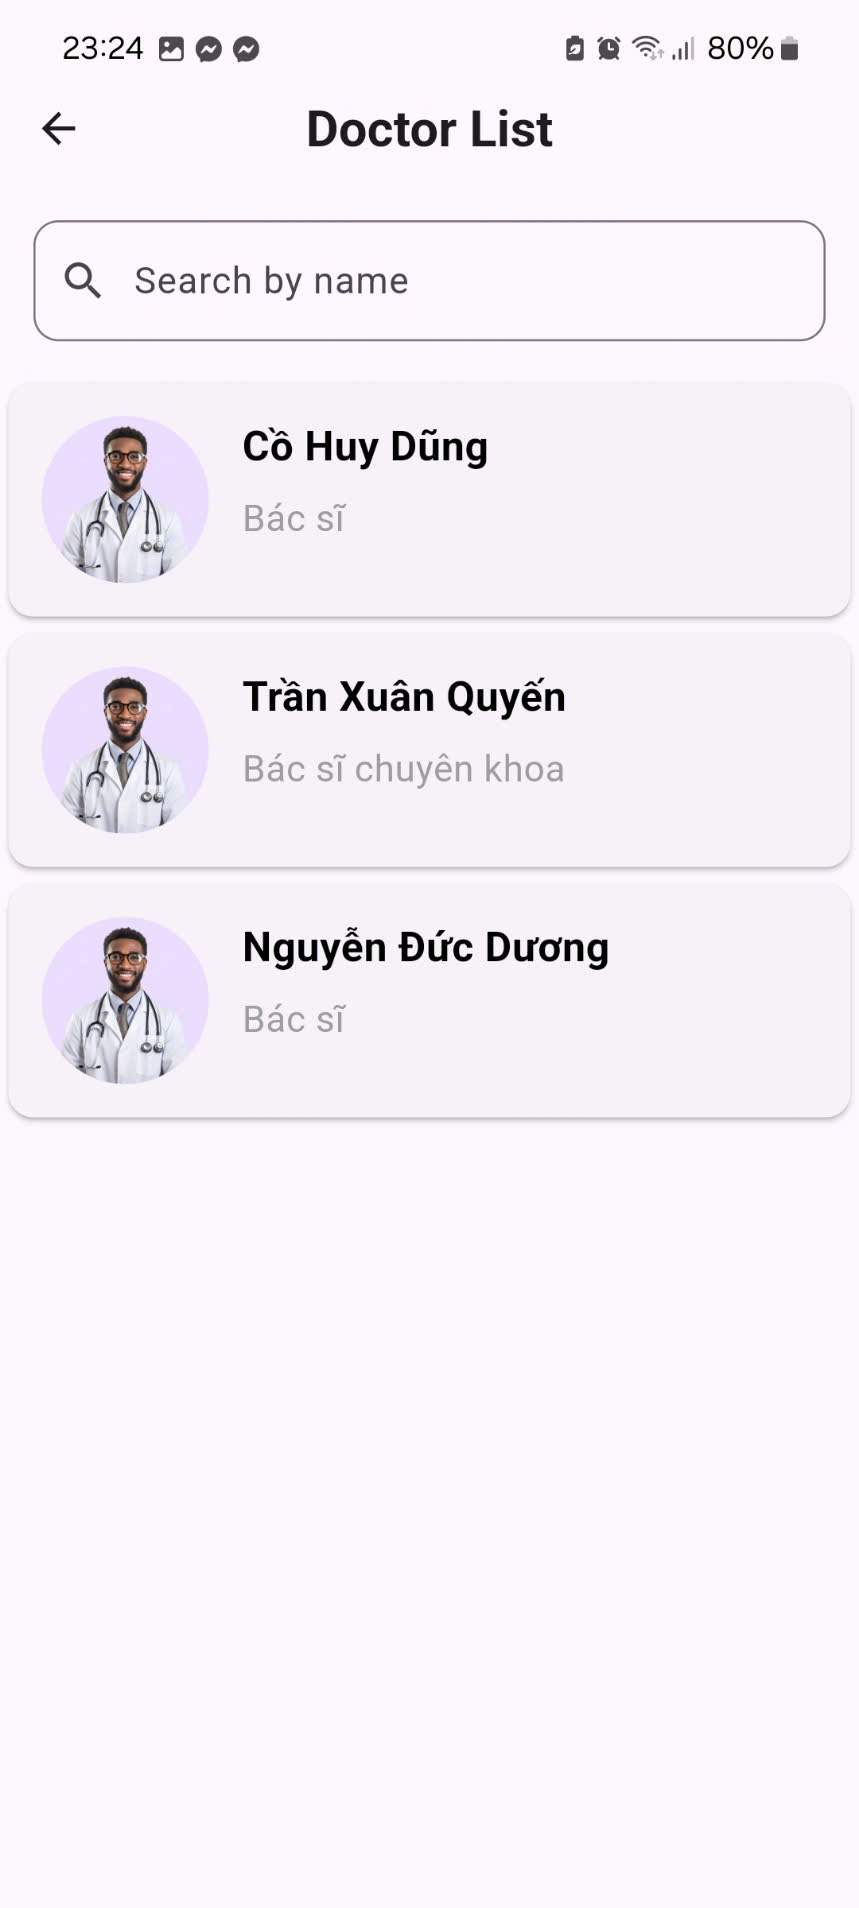
\includegraphics[width=8.5cm,height=18cm]{Images/AppUI/pickDoctor.jpg}
	\caption[Giao diện lựa chọn bác sĩ]{\bfseries \fontsize{12pt}{0pt}\selectfont Giao diện lựa chọn bác sĩ}
	\label{DoctorList}
\end{figure}
\begin{figure}[H]
	\centering
	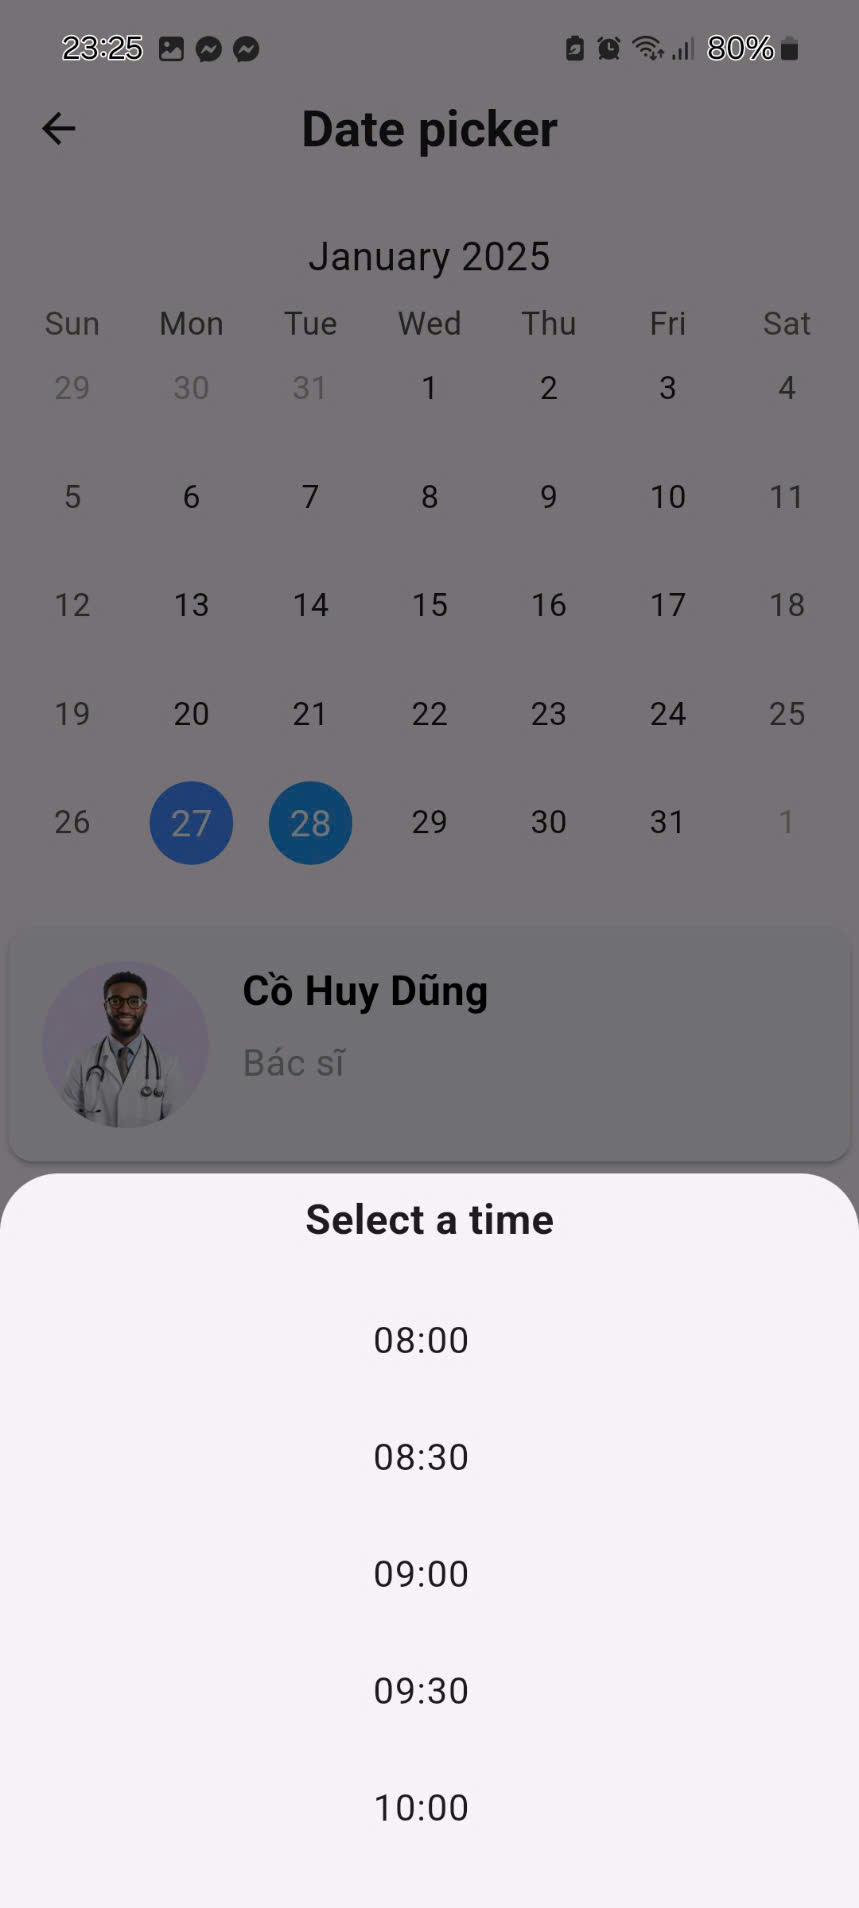
\includegraphics[width=8.5cm,height=18cm]{Images/AppUI/selectTimeWithDoctorPick.jpg}
	\caption[Giao diện chọn thời gian tương ứng với bác sĩ đã chọn trước đó]{\bfseries \fontsize{12pt}{0pt}\selectfont Giao diện chọn thời gian tương ứng với bác sĩ đã chọn trước đó}
	\label{TimePickWithDoctor}
\end{figure}

Khi đã chọn xong sẽ hiển thị Popup xác nhận đặt lịch của bệnh nhân
\begin{figure}[H]
	\centering
	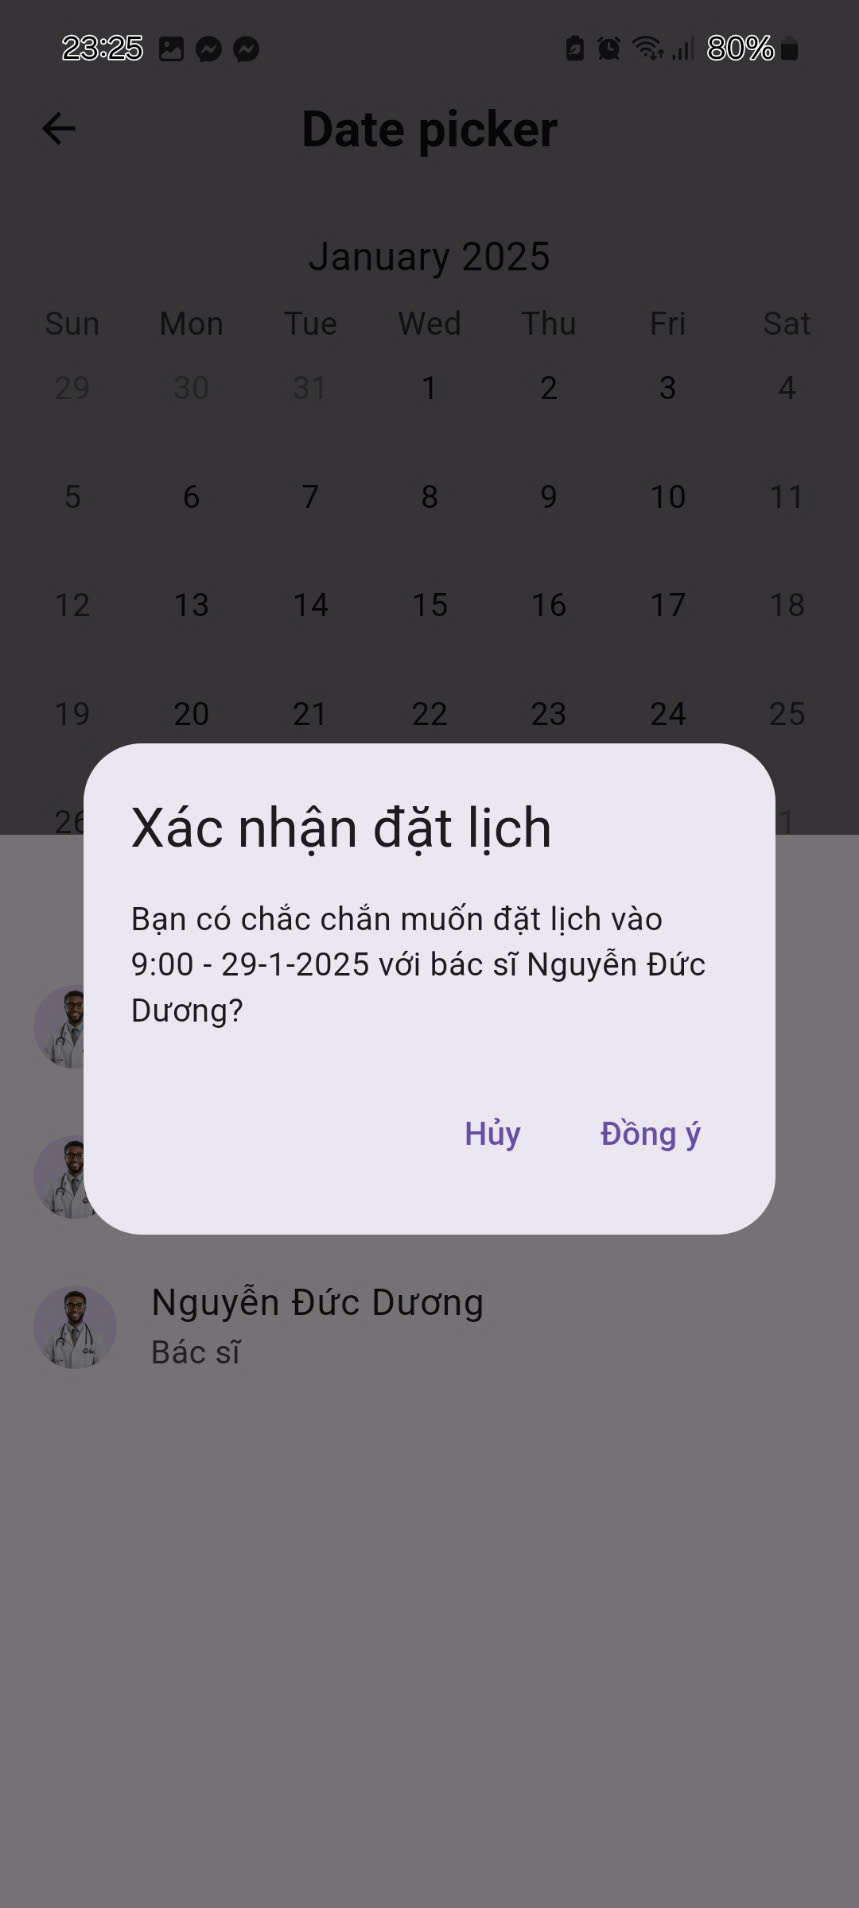
\includegraphics[width=8.5cm,height=18cm]{Images/AppUI/firmPicker.jpg}
	\caption[Popup xác nhận đặt lịch]{\bfseries \fontsize{12pt}{0pt}\selectfont Popup xác nhận đặt lịch}
	\label{TimePickWithDoctor}
\end{figure}

	Với lựa chọn thứ 2 là chọn thời gian trước, bệnh nhân sẽ đặt thời gian rảnh trước và màn hình sẽ hiển thị ra các bác sĩ đang rảnh trong thời gian đó để bệnh nhân có thể lựa chọn. Quy trình xác nhận đặt lịch tương tự như phần bên trên.

Khi đặt lịch thành công, sẽ có thông báo trả về ở phần Thông báo của cả bệnh nhân lẫn bác sĩ.
\begin{figure}[H]
	\centering
	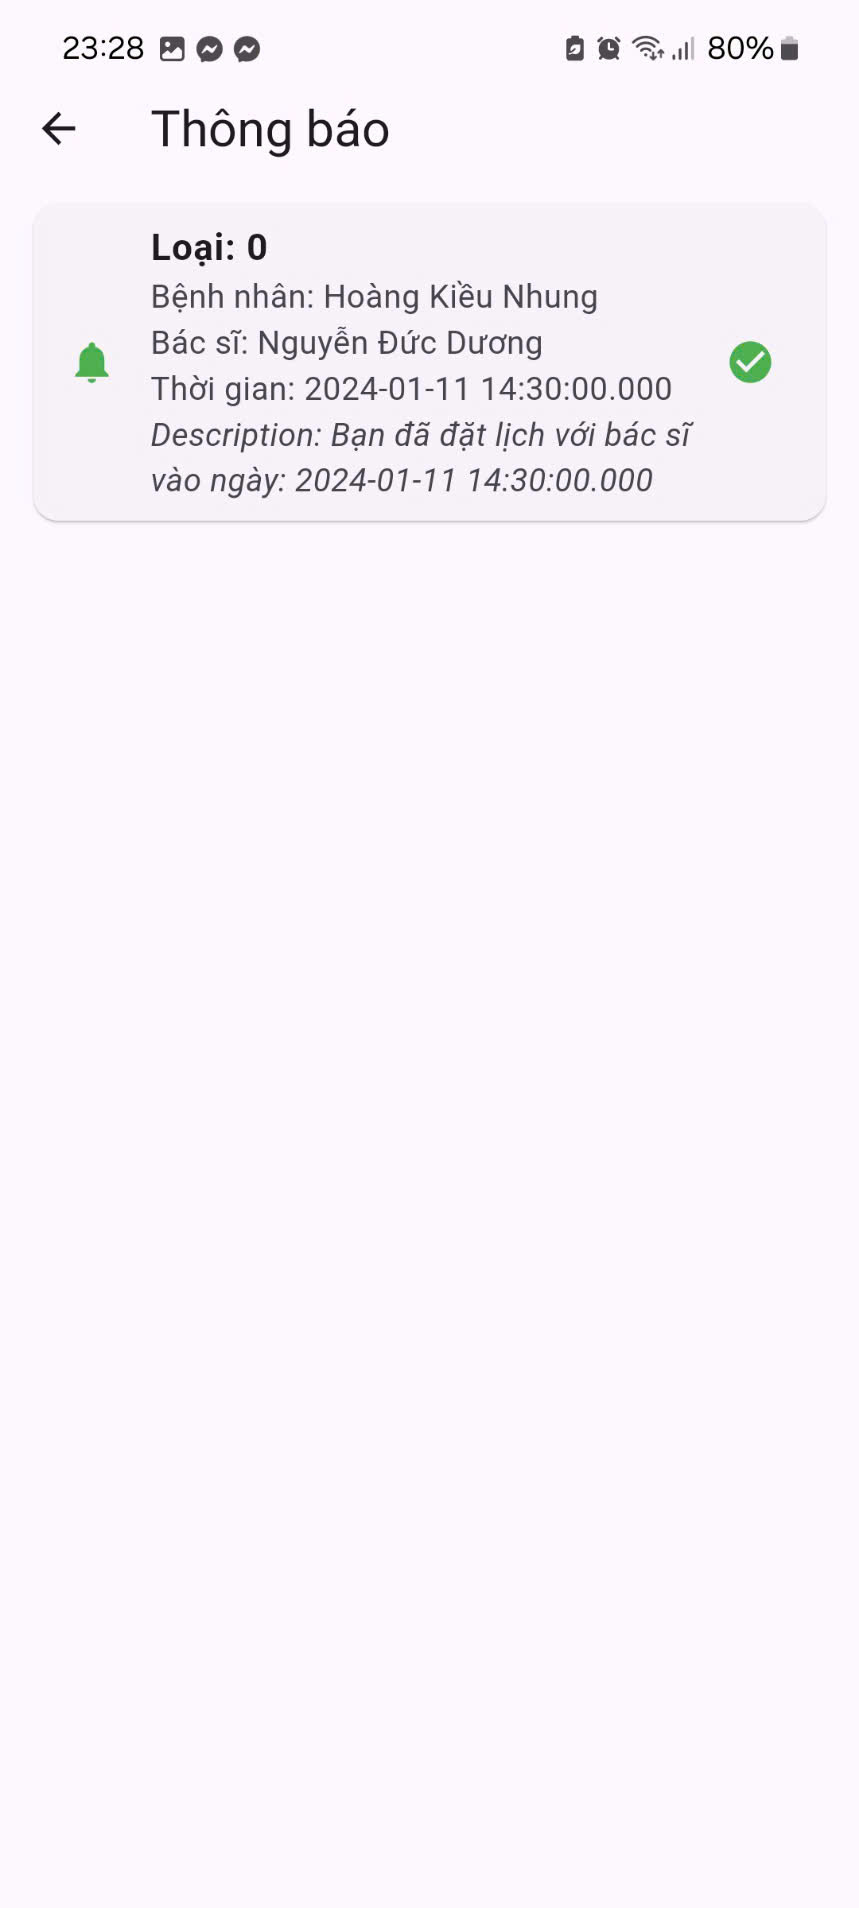
\includegraphics[width=8.5cm,height=18cm]{Images/AppUI/noti.jpg}
	\caption[Giao diện thông báo đặt lịch thành công]{\bfseries \fontsize{12pt}{0pt}\selectfont Giao diện thông báo đặt lịch thành công}
	\label{TimePickWithDoctor}
\end{figure}
Về giao diện phần Hội thoại và Thông tin cá nhân sẽ được thiết kế giống với phần giao diện bên phía bác sĩ.

\begin{figure}[H]
	\centering
	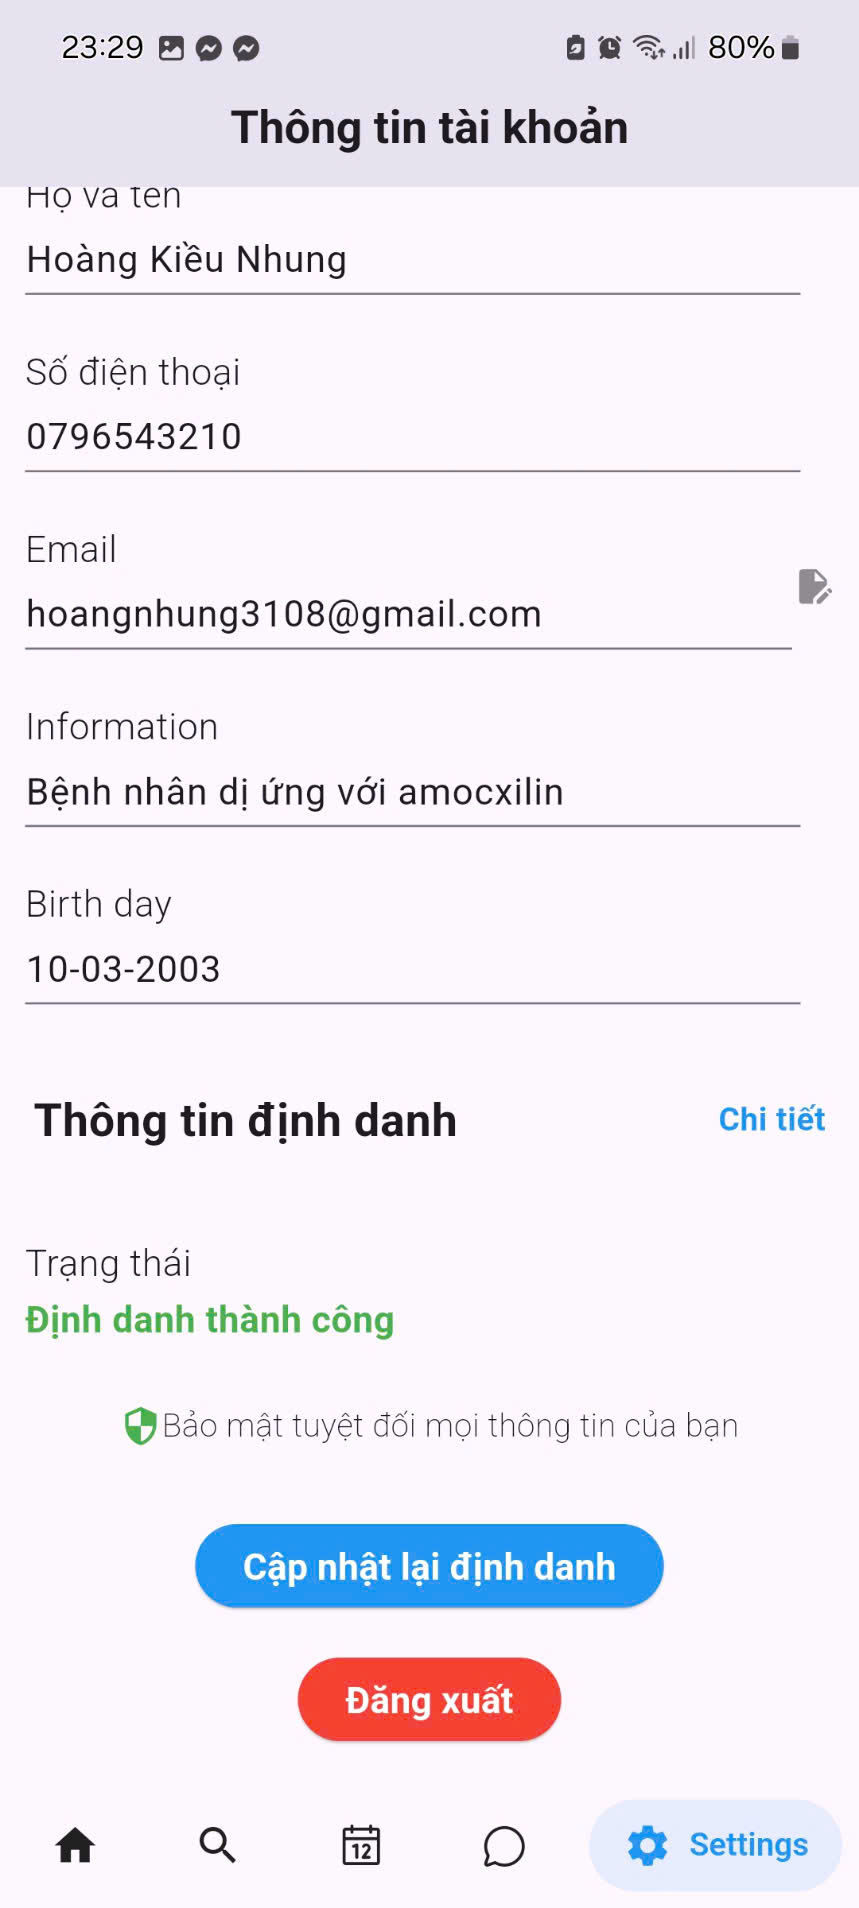
\includegraphics[width=8.5cm,height=18cm]{Images/AppUI/infoPatient.jpg}
	\caption[Giao diện thông tin cá nhân của bệnh nhân]{\bfseries \fontsize{12pt}{0pt}\selectfont Giao diện thông tin cá nhân của bệnh nhân}
	\label{TimePickWithDoctor}
\end{figure}
	\subsection{Thiết kế các chức năng}

	\subsubsection{Thiết kế các API cần thiết}


	\begin{enumerate}[a)]
		\item API xác minh tài khoản
	
		\begin{xltabular}{\textwidth}{
		  | >{\raggedright\arraybackslash}m{4.6cm}
		  | >{\centering\arraybackslash}m{2.8cm}
		  | >{\raggedright\arraybackslash}X |
		  }
		  \caption{\bfseries \fontsize{12pt}{0pt}\selectfont Bảng API xác minh tài khoản}
		  \label{table_api_auth}
		  \\
		  \hline
		  \bfseries Đường dẫn    &\bfseries Phương thức    &\bfseries Mô tả\\ \hline
		  api/ecg/auth/create-account   &   POST  & Tạo mới tài khoản người dùng \\ \hline
		  api/ecg/auth/login   &    POST    & Đăng nhập vào hệ thống \\ \hline
		  api/ecg/auth/logout   &    POST    & Đăng xuất khỏi hệ thống \\ \hline
		\end{xltabular}
	  
		\item API quản lý người dùng trong hệ thống
		\begin{xltabular}{\textwidth}{
		  | >{\raggedright\arraybackslash}m{4.6cm}
		  | >{\centering\arraybackslash}m{2.8cm}
		  | >{\raggedright\arraybackslash}X |
		  }
		  \caption{\bfseries \fontsize{12pt}{0pt}\selectfont Bảng API quản lý người dùng trong hệ thống}
		  \label{table_api_user}
		  \\
		  \hline
		  \bfseries Đường dẫn    &\bfseries Phương thức    &\bfseries Mô tả\\ \hline
		  api/ecg/users   &   GET  &  Tra cứu danh sách tất cả người dùng trong hệ thống\\  \hline
		  api/ecg/users/doctors   &   GET  &  Tra cứu danh sách toàn bộ bác sĩ trong hệ thống \\  \hline
		  api/ecg/users/:id   &   GET  &  Tra cứu dữ liệu người dùng cụ thể dựa trên id tương ứng \\  \hline
		  api/ecg/users/data/patient-data   &   GET  &  Tra cứu danh sách các bệnh nhân đang được theo dõi của bác sĩ cụ thể \\  \hline
		  api/ecg/users/data/doctor-id   &   GET  &  Tra cứu thông tin của bác sĩ phụ trách bệnh nhân \\  \hline
		  api/ecg/users/   &   PUT  &  Chỉnh sửa thông tin người dùng \\  \hline
		  api/ecg/users/:userId  &   DELETE  &  Xóa người dùng cụ thể dựa trên id tương ứng \\  \hline
		\end{xltabular}
	  
	  \item API quản lý thiết bị y tế
	  \begin{xltabular}{\textwidth}{
		| >{\raggedright\arraybackslash}m{4.8cm}
		| >{\centering\arraybackslash}m{2.8cm}
		| >{\raggedright\arraybackslash}X |
		}
		\caption{\bfseries \fontsize{12pt}{0pt}\selectfont Bảng API quản lý thiết bị y tế}
		\label{table_api_device}
		\\
		\hline
		\bfseries Đường dẫn    &\bfseries Phương thức    &\bfseries Mô tả\\ \hline
		api/ecg/device   &   GET  & Tra cứu danh sách toàn bộ thiết bị y tế trong hệ thống\\ \hline
		api/ecg/devide/:id   &    GET    & Tra cứu thông tin chi tiết của một thiết bị y tế dựa trên id tương ứng \\ \hline
		api/ecg/device/add &   POST     & Thêm mới thiết bị y tế \\ \hline
		api/ecg/device/update  &     PUT   & Cập nhật thông tin chi tiết cho thiết bị y tế cụ thể \\ \hline
		api/ecg/device/:deviceId  &     DELETE   & Xóa thiết bị y tế dựa trên id tương ứng \\ \hline
	  \end{xltabular}
	  
	  \item API quản lý dữ liệu phiên đo
	  \begin{xltabular}{\textwidth}{
		| >{\raggedright\arraybackslash}p{5cm}
		| >{\centering\arraybackslash}m{2.8cm}
		| >{\raggedright\arraybackslash}X |
		}
		\caption{\bfseries \fontsize{12pt}{0pt}\selectfont Bảng API quản lý dữ liệu phiên đo}
		\label{table_api_record}
		\\
		\hline
		\bfseries Đường dẫn    &\bfseries Phương thức    &\bfseries Mô tả \\ \hline
		 api/ecg/records   &   GET  & Tra cứu danh sách các dữ liệu phiên đo \\ \hline
		 api/ecg/records/:id   &    GET    & Tra cứu dữ liệu phiên đo cụ thể dựa theo id tương ứng \\ \hline
		 api/ecg/records/data/ doctor &   GET     & Tra cứu danh sách các dữ liệu phiên đo của bệnh nhân mà bác sĩ phụ trách \\ \hline
		 api/ecg/records/data/ patient &   GET     & Tra cứu danh sách dữ liệu các phiên đo cá nhân \\ \hline
		 api/ecg/records/   &    POST    & Tạo dữ liệu phiên đo mới \\ \hline
		 api/ecg/records/   &    PUT    & Cập nhật dữ liệu phiên đo \\ \hline
		 api/ecg/records/:recordId  &    DELETE    & Xóa dữ liệu phiên đo dựa theo id tương ứng \\ \hline
		\end{xltabular}
	  
	  
	  \item API quản lý dịch vụ lịch khám
	  \begin{xltabular}{\textwidth}{
		| >{\raggedright\arraybackslash}m{4.5cm}
		| >{\centering\arraybackslash}m{2.8cm}
		| >{\raggedright\arraybackslash}X |
		}
		\caption{\bfseries \fontsize{12pt}{0pt}\selectfont Bảng API quản lý dịch vụ lịch khám}
		\label{table_api_schedule}
		\\
		\hline
		\bfseries Đường dẫn    &\bfseries Phương thức    &\bfseries Mô tả\\ \hline
		api/ecg/schedules   &   GET  & Tra cứu danh sách tất cả lịch khám trong hệ thống \\ \hline
		api/ecg/schedules/ doctor-id  &    GET    & Tra cứu danh sách lịch khám của bác sĩ cụ thể \\ \hline
		api/ecg/schedules/ patient-id  &    GET    & Tra cứu danh sách lịch khám của bệnh nhân cụ thể \\ \hline
		api/ecg/schedules/create-by-doctor  &    POST    & Cho phép bác sĩ đặt lịch tái khám cho bệnh nhân \\ \hline
		api/ecg/schedules/create-by-patient  &    POST    & Cho phép bệnh nhân đặt lịch khám với bác sĩ \\ \hline
		api/ecg/schedules/time/ available-doctor/: schedule-time  &    GET    & Tra cứu danh sách các bác sĩ khả dụng theo thời gian đã chọn \\ \hline
		api/ecg/schedules/ available-schedule/:id  &    GET    & Tra cứu các khung giờ trống có thể đặt lịch với bác sĩ cụ thể. \\ \hline
		api/ecg/schedules/accept-schedule  &    PUT    & Chấp nhận lịch khám cụ thể \\ \hline
		api/ecg/schedules/reject-schedule/:id  &    DELETE    & Từ chối lịch khám cụ thể \\ \hline
		\end{xltabular}
	  
	  \item API liên quan đến chẩn đoán cho bệnh nhân
	  \begin{xltabular}{\textwidth}{
		| >{\raggedright\arraybackslash}m{4.5cm}
		| >{\centering\arraybackslash}m{2.8cm}
		| >{\raggedright\arraybackslash}X |
		}
		\caption{\bfseries \fontsize{12pt}{0pt}\selectfont Bảng API liên quan đến chẩn đoán cho bệnh nhân}
		\label{table_api_diagnosis}
		\\
		\hline
		\bfseries Đường dẫn    &\bfseries Phương thức    &\bfseries Mô tả\\ \hline
		api/ecg/diagnosis   &   POST  & Tạo chẩn đoán mới cho bệnh nhân \\ \hline
		api/ecg/diagnosis/ schedule/:scheduleId   &   POST  & Tra cứu thông tin chẩn đoán dựa trên id lịch khám tương ứng\\ \hline
		api/ecg/diagnosis/update   &   POST  & Cập nhật thông tin chẩn đoán \\ \hline
		\end{xltabular}
	  
	  
	  \item API liên quan đến thông báo về lịch khám
	  \begin{xltabular}{\textwidth}{
		| >{\raggedright\arraybackslash}m{4.5cm}
		| >{\centering\arraybackslash}m{2.8cm}
		| >{\raggedright\arraybackslash}X |
		}
		\caption{\bfseries \fontsize{12pt}{0pt}\selectfont Bảng API liên quan đến thông báo về lịch khám}
		\label{table_api_notification}
		\\
		\hline
		\bfseries Đường dẫn    &\bfseries Phương thức    &\bfseries Mô tả\\ \hline
		api/ecg/notification/get   &   GET  & Tra cứu tất cả các thông báo của người dùng cụ thể  \\ \hline
		api/ecg/notification   &   POST  & Tạo thông báo mới liên quan đến lịch khám \\ \hline
		api/ecg/notification/ update-seen   &   POST  & Cập nhật trạng thái thông báo đã được xem\\ \hline
		api/ecg/notification/:id   &   DELETE  & Xóa thông báo dựa trên id tương ứng\\ \hline
		\end{xltabular}
	  
	  \item API liên quan đến tin nhắn
	  \begin{xltabular}{\textwidth}{
		| >{\raggedright\arraybackslash}m{4.5cm}
		| >{\centering\arraybackslash}m{2.8cm}
		| >{\raggedright\arraybackslash}X |
		}
		\caption{\bfseries \fontsize{12pt}{0pt}\selectfont Bảng API liên quan đến tin nhắn}
		\label{table_api_chat}
		\\
		\hline
		\bfseries Đường dẫn    &\bfseries Phương thức    &\bfseries Mô tả\\ \hline
		api/ecg/groupChat   &   POST  & Tạo nhóm trò chuyện mới  \\ \hline
		api/ecg/groupChat   &   GET  & Tra cứu danh sách các nhóm trò chuyện của người dùng  \\ \hline
		api/ecg/chat/messages/: groupChatId   &   GET  & Tra cứu lịch sử trò chuyện của các đoạn hội thoại đã thực hiện \\ \hline
		api/ecg/chat/send   &   POST  & Cho phép người dùng gửi tin nhắn đến các đối tượng liên quan \\ \hline
		\end{xltabular}
	\end{enumerate}
	
	
	\subsubsection{Sơ đồ tuần tự API}
Phần này cung cấp các sơ đồ tuần tự minh họa chi tiết cách thức hoạt động của các API trong hệ thống.
Dựa trên bảng API đã thiết kế, các sơ đồ tuần tự sẽ mô phỏng luồng xử lý từ khi nhận yêu cầu đến khi trả về kết quả cho người dùng,
cho thấy rõ sự tương tác giữa các thành phần và lớp chức năng trong hệ thống.
% ------------------------Auth----------------------

\paragraph{Các API phục vụ mục đích xác minh tài khoản}
\mbox{}

\begin{figure}[H]
	\centering
	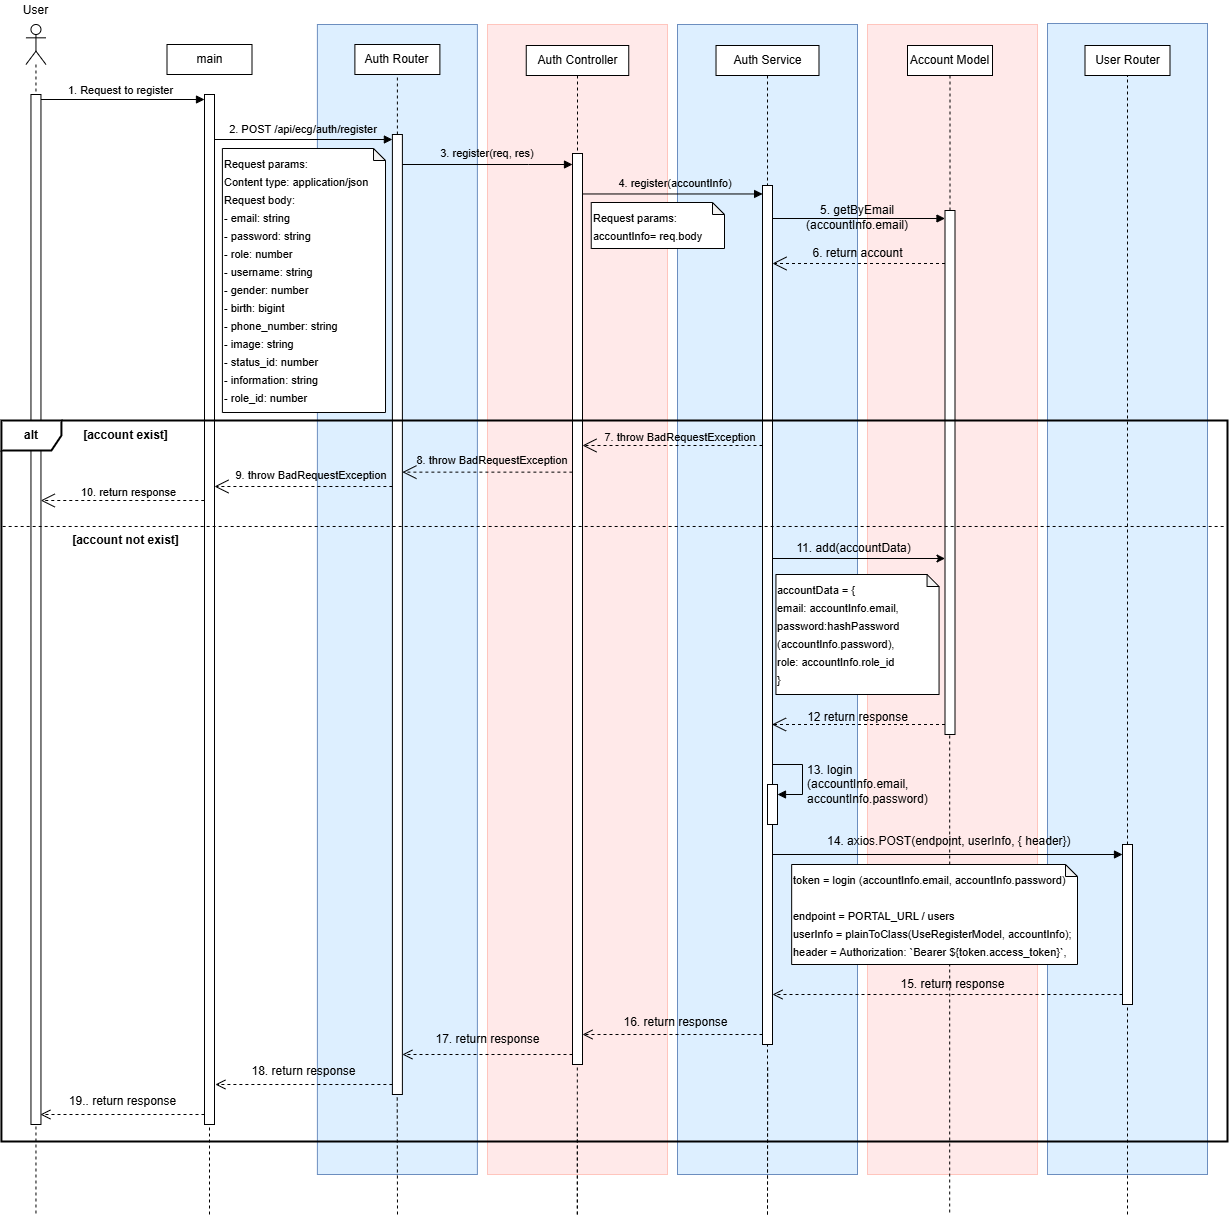
\includegraphics[width=16cm]{Images/api_sequence/authen/authentication-register.drawio.png}
	\caption[Sơ đồ tuần tự API tạo mới tài khoản người dùng]{\bfseries \fontsize{12pt}{0pt}\selectfont Sơ đồ tuần tự API tạo mới tài khoản người dùng}
	\label{sequence_diagram_create_account}
\end{figure}

\begin{figure}[H]
	\centering
	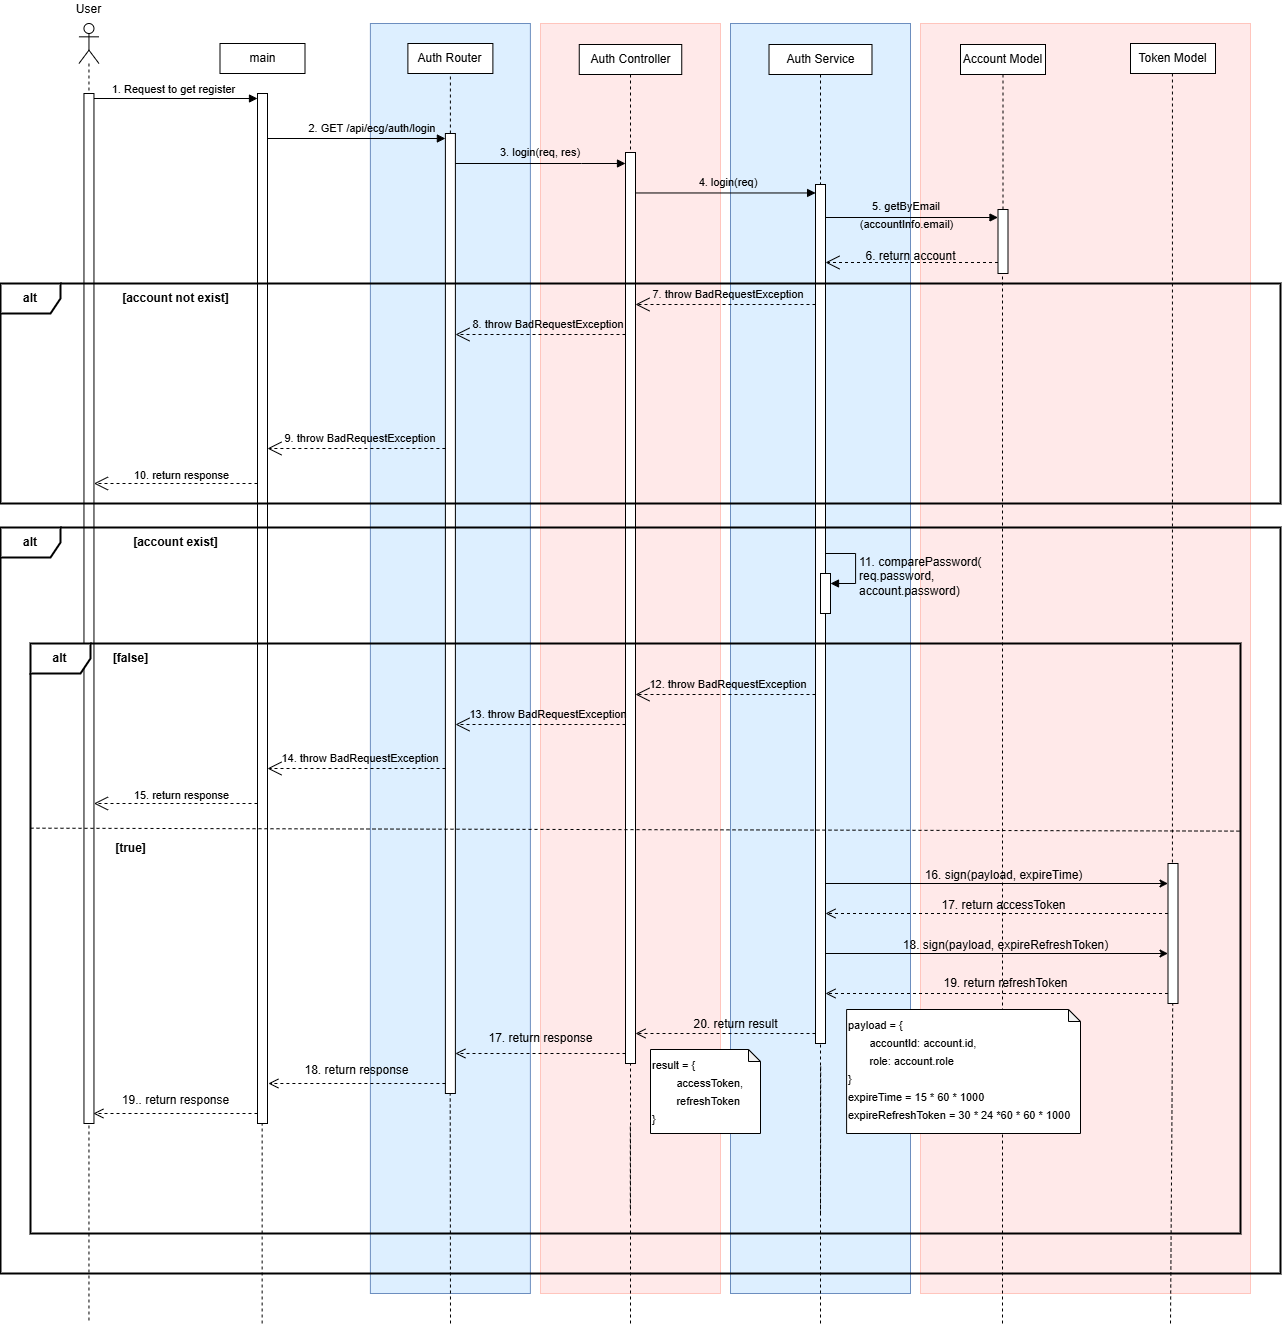
\includegraphics[width=16cm]{Images/api_sequence/authen/authentication-login.drawio.png}
	\caption[Sơ đồ tuần tự API đăng nhập vào hệ thống]{\bfseries \fontsize{12pt}{0pt}\selectfont Sơ đồ tuần tự API đăng nhập vào hệ thống}
	\label{sequence_diagram_login}
\end{figure}


% % ------------------------User----------------------
\paragraph{Các API phục vụ mục đích quản lý người dùng trong hệ thống}
\mbox{}
\begin{figure}[H]
	\centering
	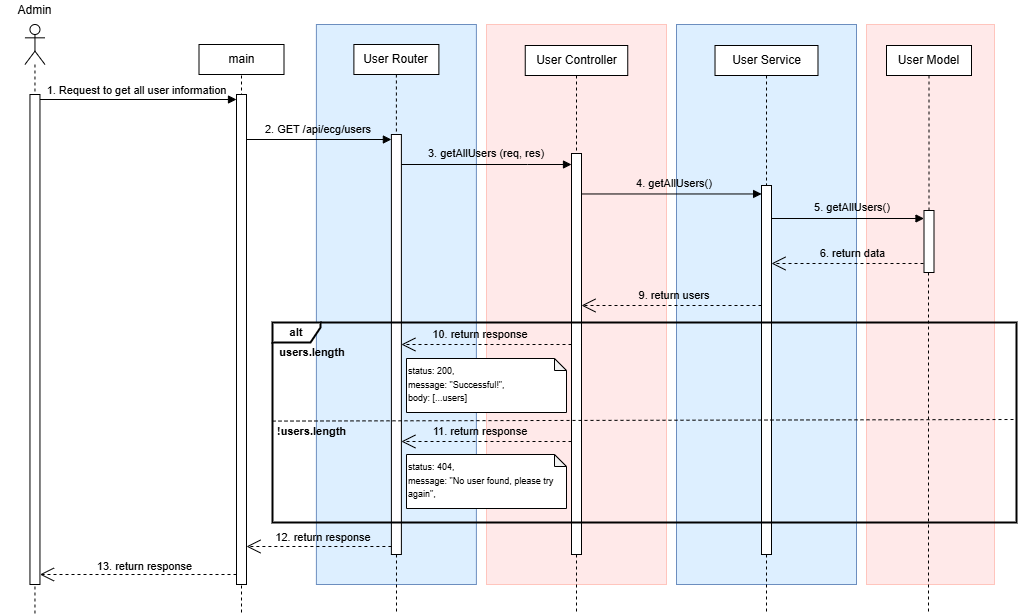
\includegraphics[width=16cm]{Images/api_sequence/user/getAllUsers.drawio.png}
	\caption[Sơ đồ tuần tự API tra cứu danh sách tất cả người dùng trong hệ thống]{\bfseries \fontsize{12pt}{0pt}\selectfont Sơ đồ tuần tự API tra cứu danh sách tất cả người dùng trong hệ thống}
	\label{sequence_diagram_get_all_users}
\end{figure}

\begin{figure}[H]
	\centering
	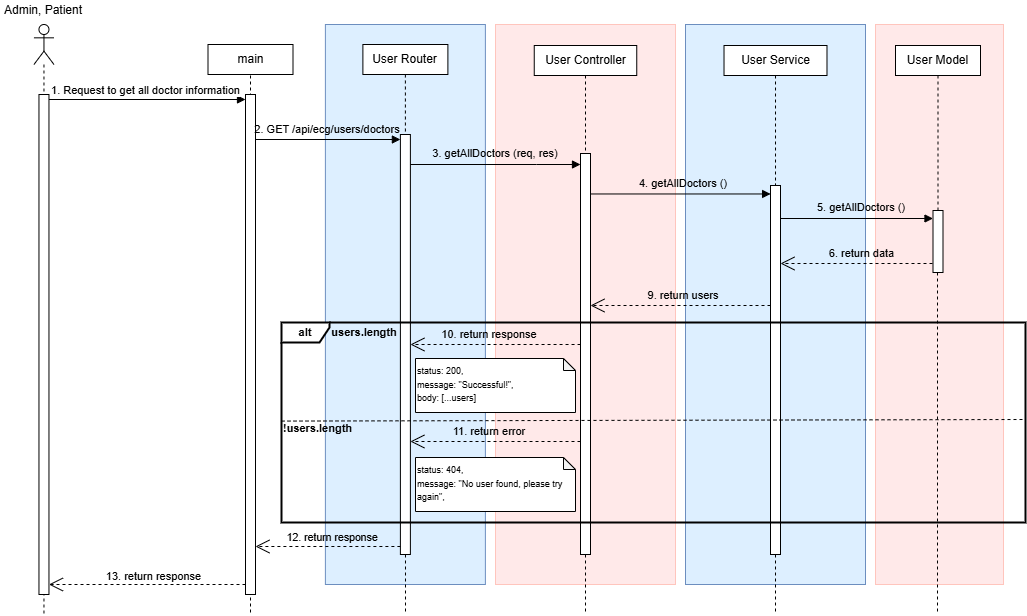
\includegraphics[width=16cm]{Images/api_sequence/user/getAllDoctors.drawio.png}
	\caption[Sơ đồ tuần tự API tra cứu danh sách toàn bộ bác sĩ trong hệ thống]{\bfseries \fontsize{12pt}{0pt}\selectfont Sơ đồ tuần tự API tra cứu danh sách toàn bộ bác sĩ trong hệ thống}
	\label{sequence_diagram_get_all_doctors}
\end{figure}

\begin{figure}[H]
	\centering
	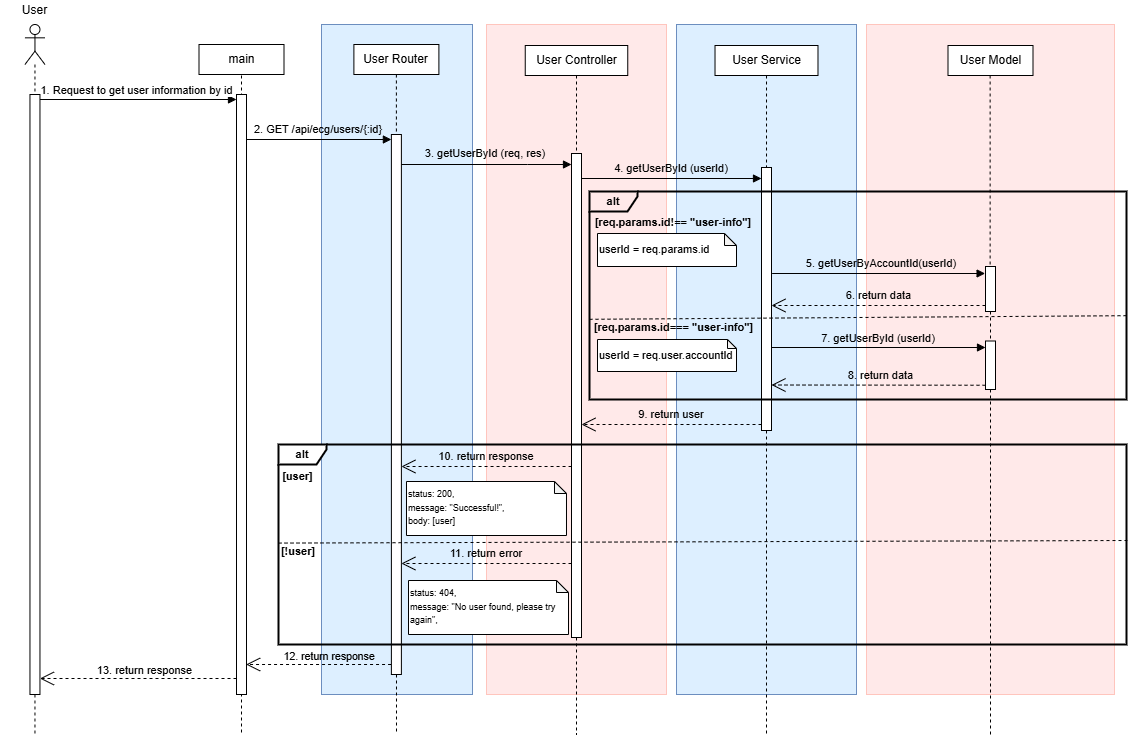
\includegraphics[width=16cm]{Images/api_sequence/user/getUserById.drawio.png}
	\caption[Sơ đồ tuần tự API tra cứu của thông tin người dùng cụ thể dựa trên id tương ứng]{\bfseries \fontsize{12pt}{0pt}\selectfont Sơ đồ tuần tự API tra cứu thông tin của người dùng cụ thể dựa trên id tương ứng}
	\label{sequence_diagram_get_user_by_id}
\end{figure}

\begin{figure}[H]
	\centering
	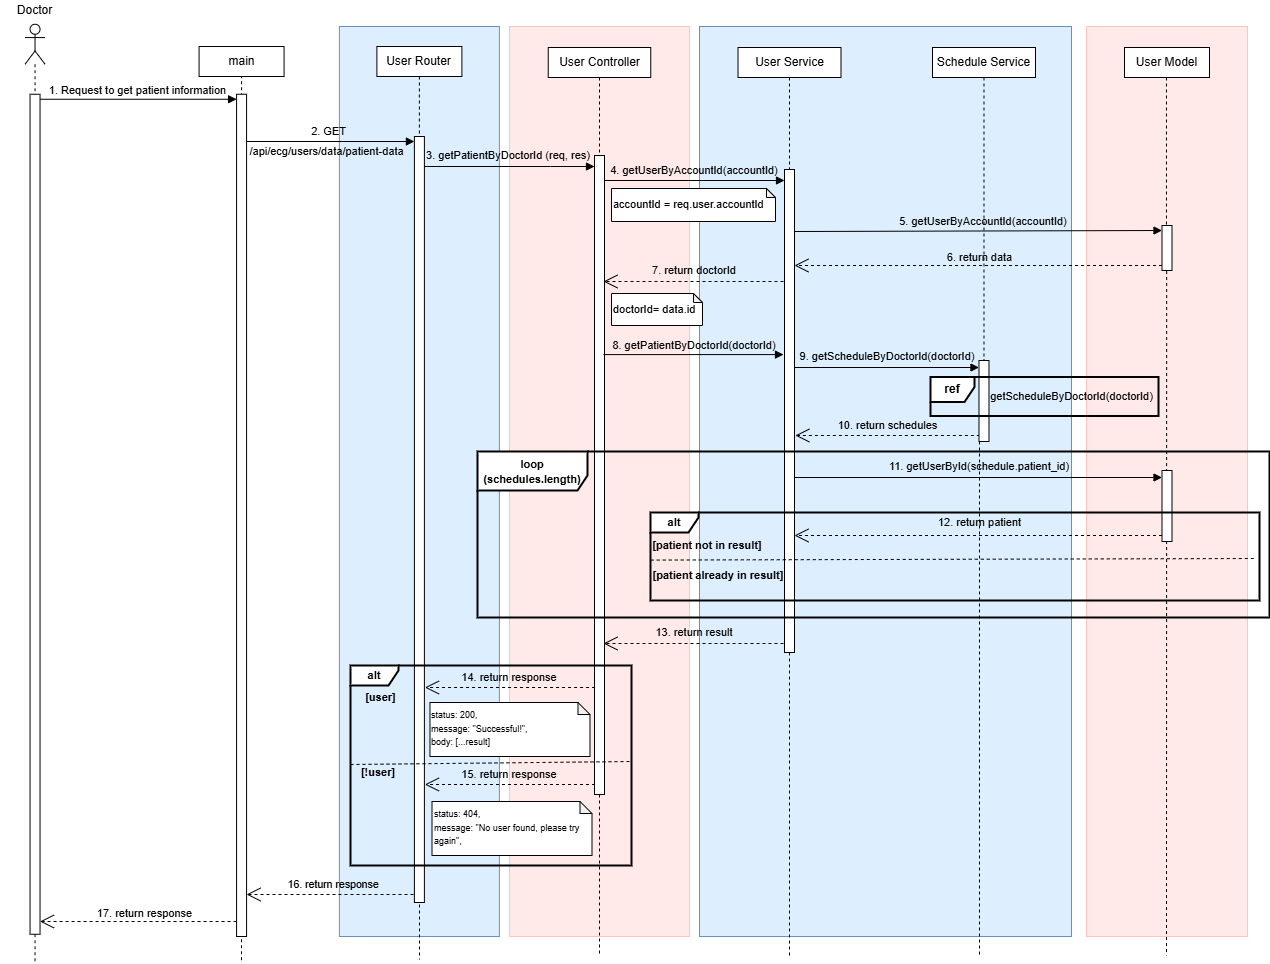
\includegraphics[width=16cm]{Images/api_sequence/user/getPatientByDoctorId.drawio.png}
	\caption[Sơ đồ tuần tự API tra cứu danh sách bệnh nhân đang được theo dõi của bác sĩ cụ thể]{\bfseries \fontsize{12pt}{0pt}\selectfont Sơ đồ tuần tự API tra cứu danh sách bệnh nhân đang được theo dõi của bác sĩ cụ thể}
	\label{sequence_diagram_get_patient_data}
\end{figure}

\begin{figure}[H]
	\centering
	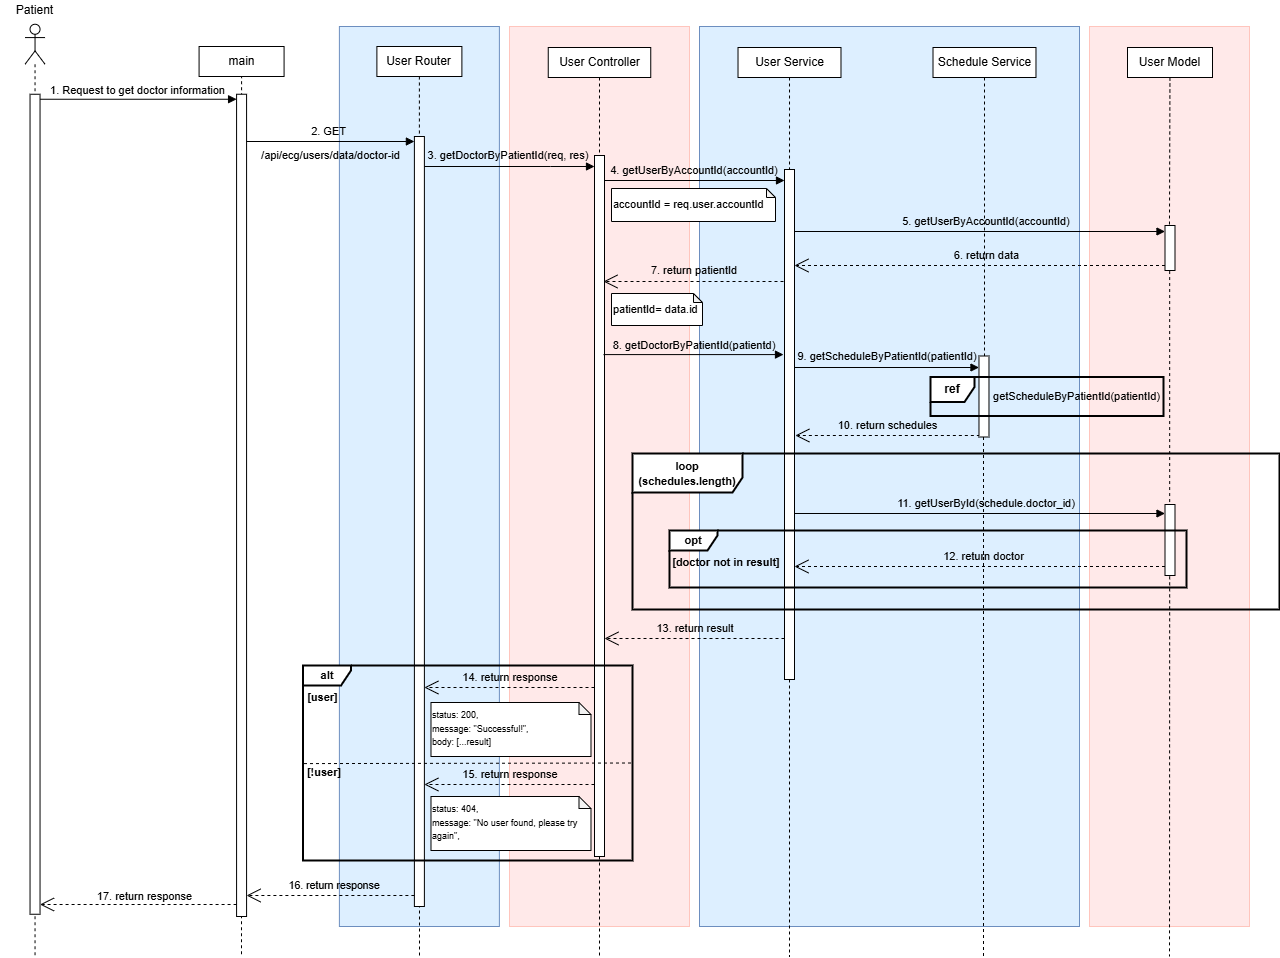
\includegraphics[width=16cm]{Images/api_sequence/user/getDoctorByPatientId.drawio.png}
	\caption[Sơ đồ tuần tự API tra cứu thông tin của bác sĩ phụ trách bệnh nhân]{\bfseries \fontsize{12pt}{0pt}\selectfont Sơ đồ tuần tự API tra cứu thông tin của bác sĩ phụ trách bệnh nhân}
	\label{sequence_diagram_get_doctor_data}
\end{figure}

\begin{figure}[H]
	\centering
	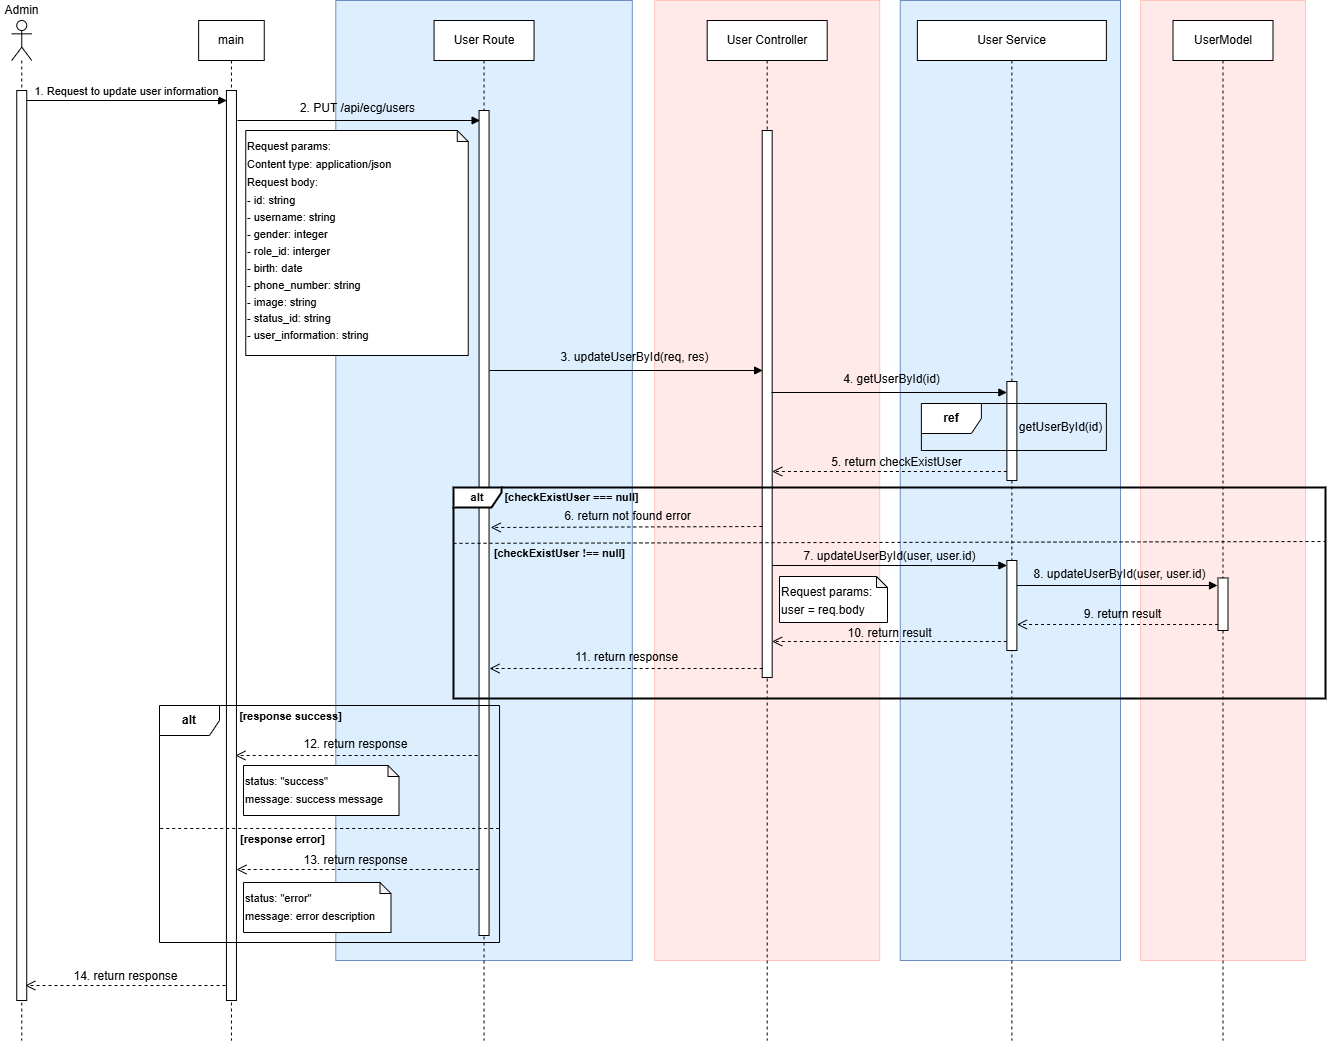
\includegraphics[width=16cm]{Images/api_sequence/user/updateUserById.drawio.png}
	\caption[Sơ đồ tuần tự API chỉnh sửa thông tin của người dùng]{\bfseries \fontsize{12pt}{0pt}\selectfont Sơ đồ tuần tự API thay đổi thông tin của người dùng}
	\label{sequence_diagram_update_user}
\end{figure}

\begin{figure}[H]
	\centering
	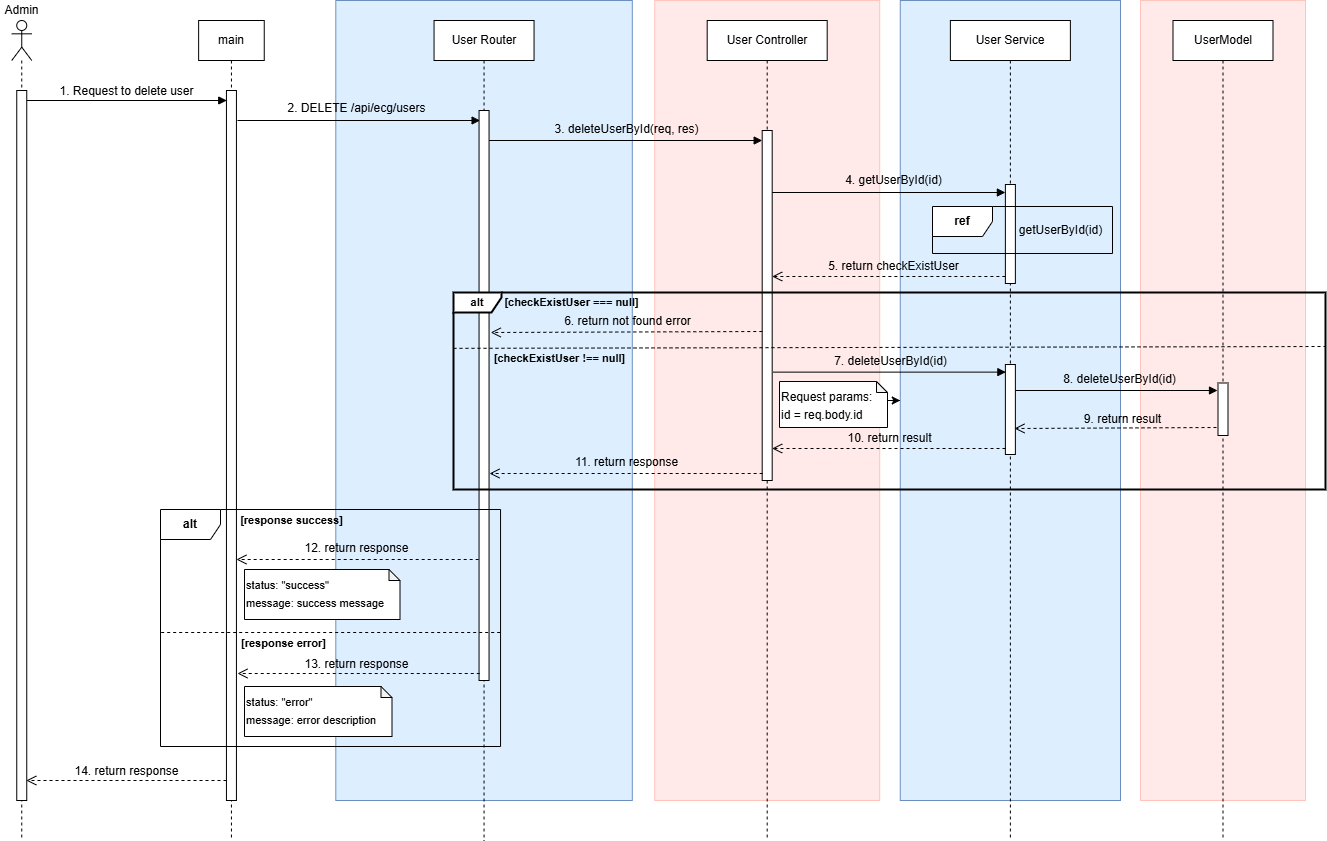
\includegraphics[width=16cm]{Images/api_sequence/user/deleteUserById.drawio.png}
	\caption[Sơ đồ tuần tự API xóa người dùng cụ thể dựa trên id tương ứng]{\bfseries \fontsize{12pt}{0pt}\selectfont Sơ đồ tuần tự API xóa người dùng cụ thể dựa trên id tương ứng}
	\label{sequence_diagram_delete_user}
\end{figure}

% % ------------------------Device----------------------
\paragraph{Các API phục vụ mục đích quản lý thiết bị y tế}
\mbox{}
\begin{figure}[H]
	\centering
	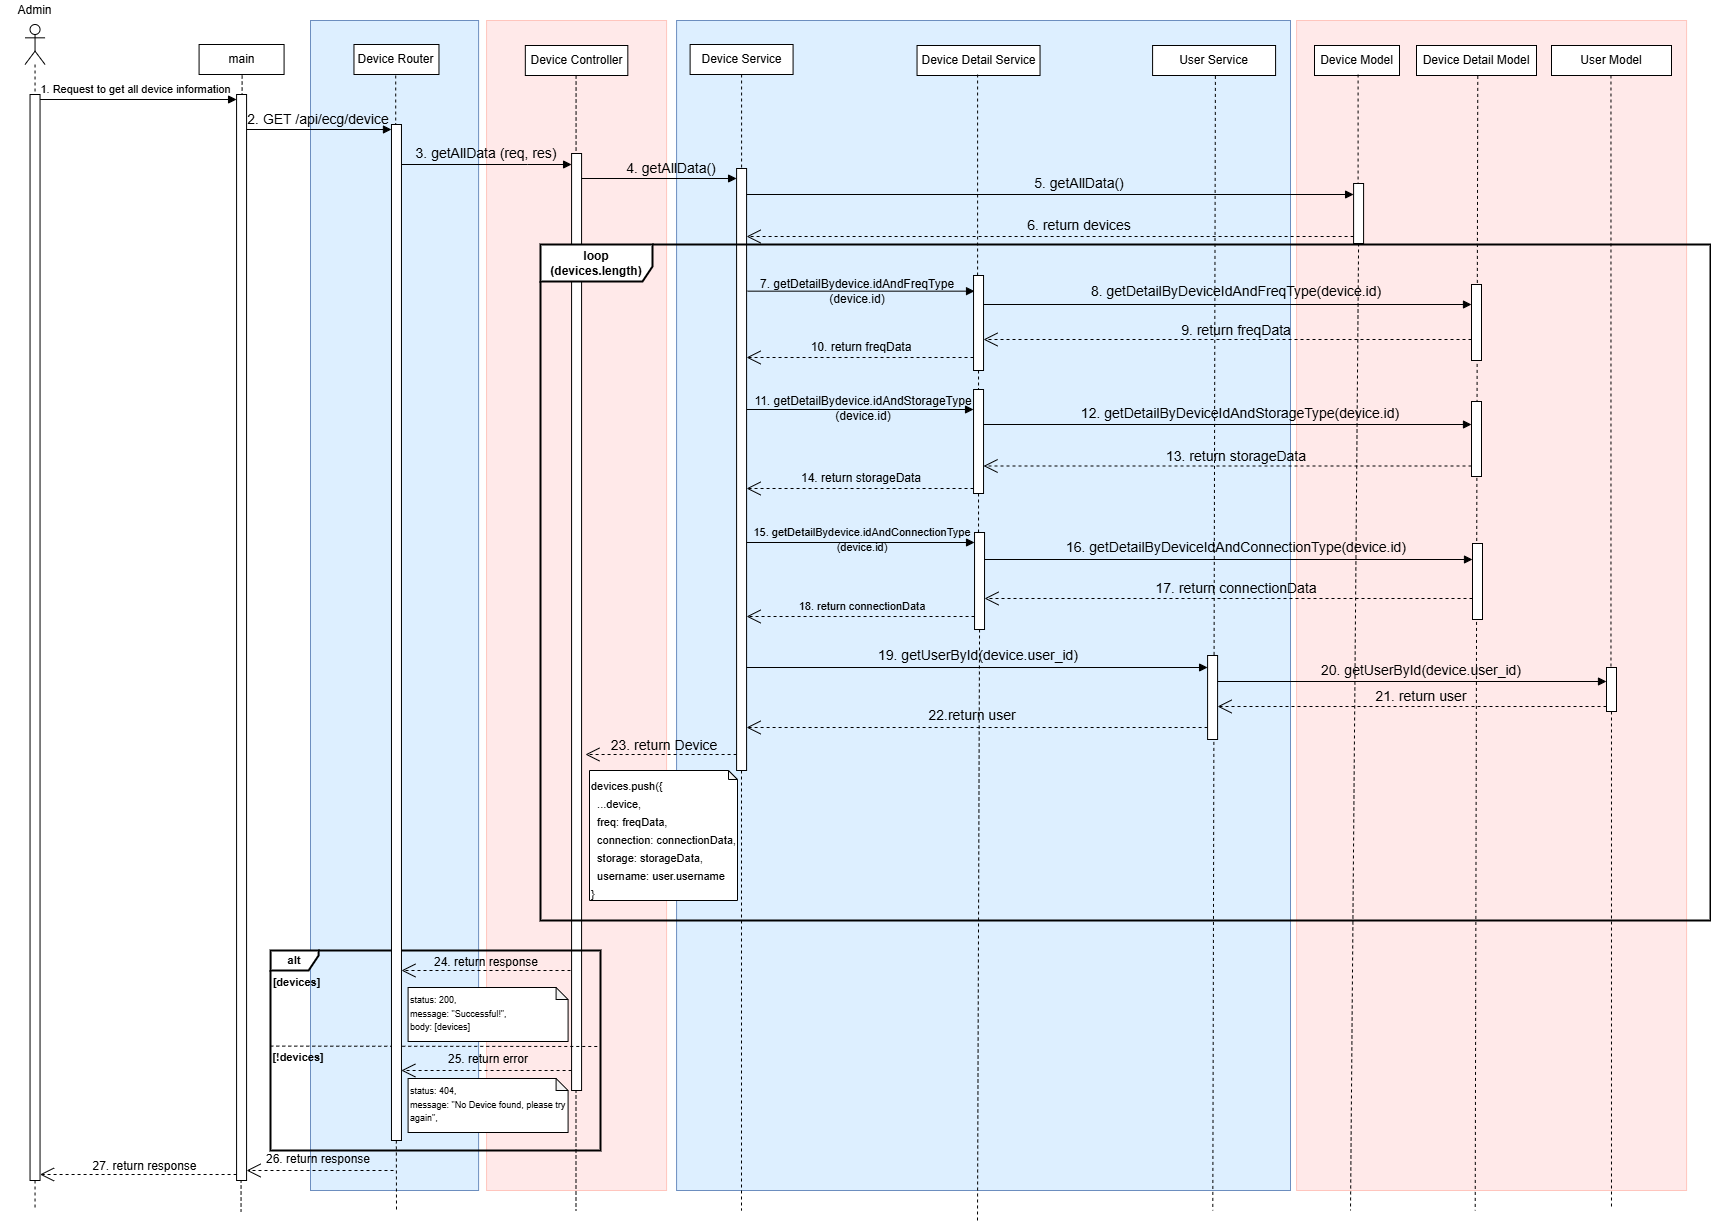
\includegraphics[width=16cm]{Images/api_sequence/device/device-GetAllDevice.drawio.png}
	\caption[Sơ đồ tuần tự API tra cứu danh sách toàn bộ thiết bị y tế trong hệ thống]{\bfseries \fontsize{12pt}{0pt}\selectfont Sơ đồ tuần tự API tra cứu danh sách toàn bộ thiết bị y tế trong hệ thống}
	\label{sequence_diagram_get_all_devices}
\end{figure}

\begin{figure}[H]
	\centering
	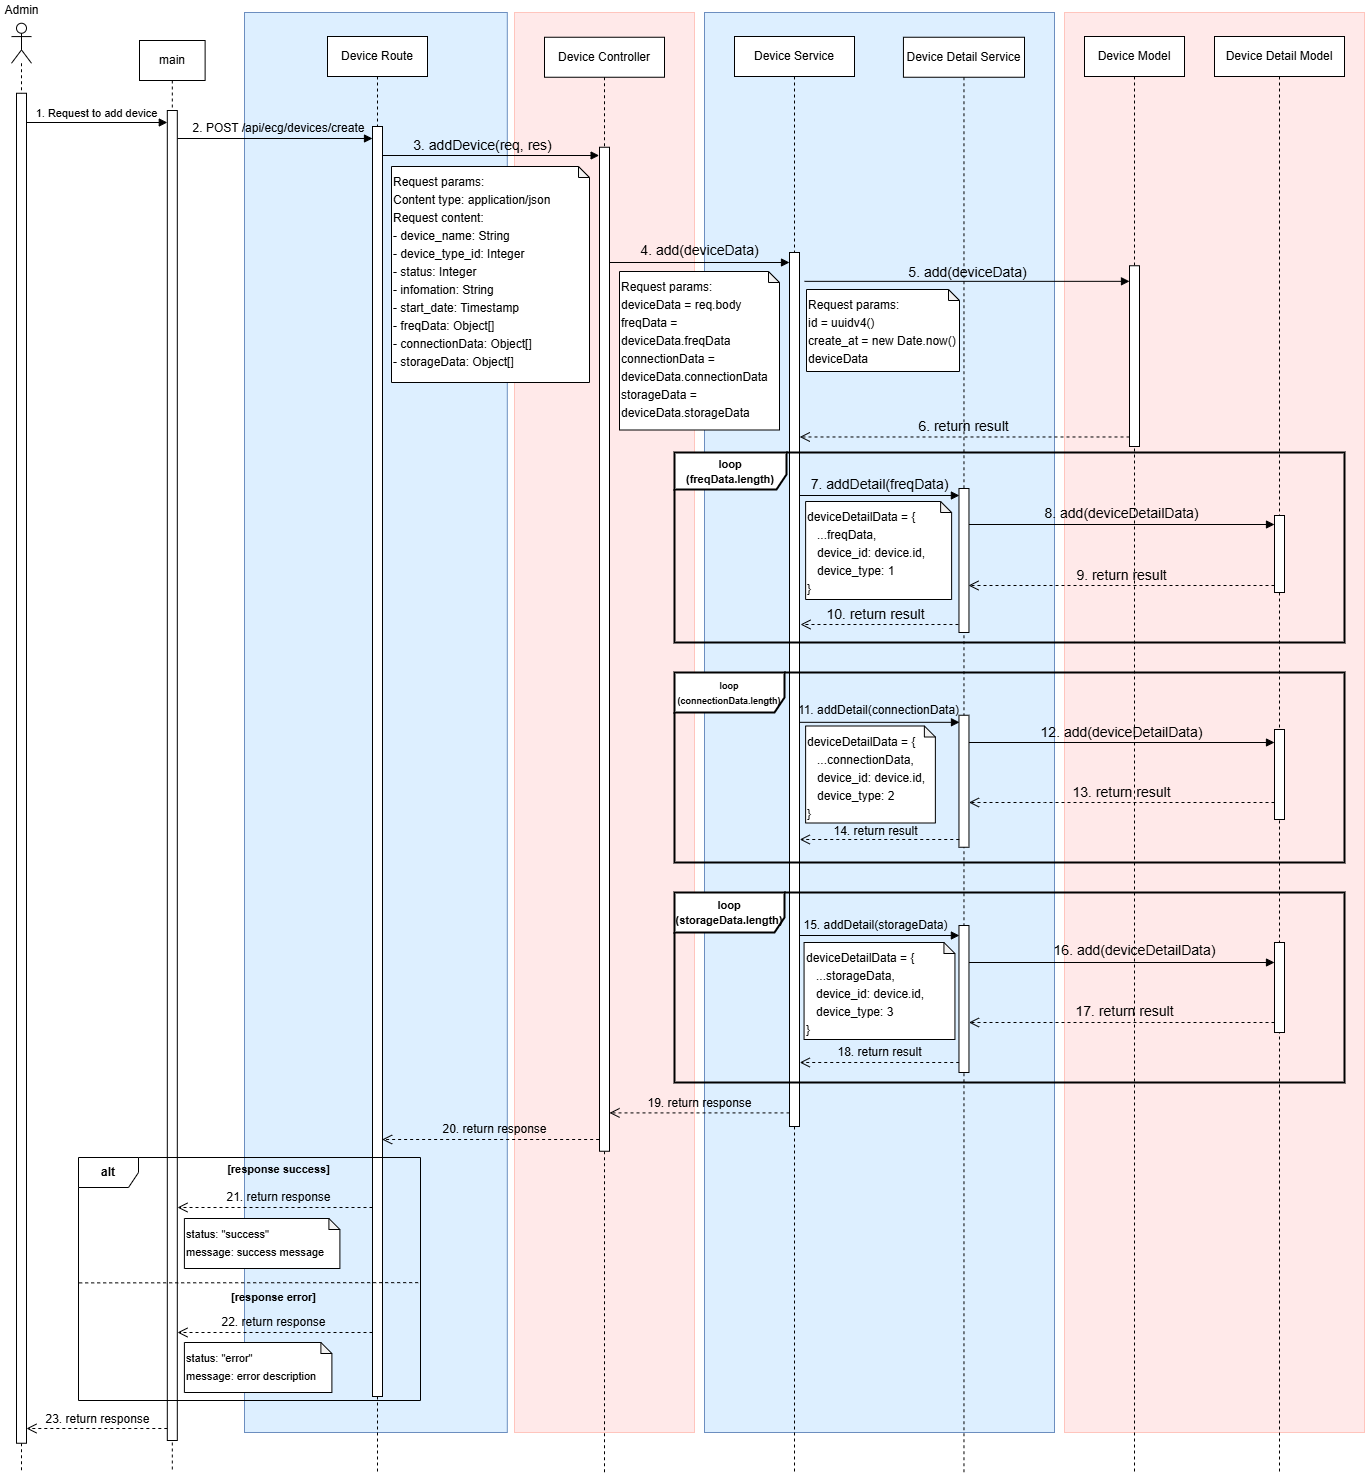
\includegraphics[width=16cm]{Images/api_sequence/device/device-Add.drawio.png}
	\caption[Sơ đồ tuần tự API thêm mới thiết bị y tế]{\bfseries \fontsize{12pt}{0pt}\selectfont Sơ đồ tuần tự API thêm mới thiết bị y tế}
	\label{sequence_diagram_add_device}
\end{figure}

\begin{figure}[H]
	\centering
	\includegraphics[width=16cm]{Images/api_sequence/device/device-GetDeviceById.drawio.png}
	\caption[Sơ đồ tuần tự API tra cứu thông tin chi tiết một thiết bị y tế dựa trên id tương ứng]{\bfseries \fontsize{12pt}{0pt}\selectfont Sơ đồ tuần tự API tra cứu thông tin chi tiết một thiết bị y tế dựa trên id tương ứng}
	\label{sequence_diagram_add_device}
\end{figure}

\begin{figure}[H]
	\centering
	\includegraphics[width=16cm]{Images/api_sequence/device/device-updateDevice.drawio.png}
	\caption[ Sơ đồ tuần tự API chỉnh sửa thông tin chi tiết cho thiết bị y tế cụ thể]{\bfseries \fontsize{12pt}{0pt}\selectfont  Sơ đồ tuần tự API chỉnh sửa thông tin chi tiết cho thiết bị y tế cụ thể}
	\label{sequence_diagram_update_device}
\end{figure}

\begin{figure}[H]
	\centering
	\includegraphics[width=16cm]{Images/api_sequence/device/device-Add.drawio.png}
	\caption[Sơ đồ tuần tự API xóa thiết bị y tế dựa trên id tương ứng]{\bfseries \fontsize{12pt}{0pt}\selectfont Sơ đồ tuần tự API xóa thiết bị y tế dựa trên id tương ứng}
	\label{sequence_diagram_get_device_by_id}
\end{figure}
% % ------------------------Record----------------------
\paragraph{Các API phục vụ mục đích liên quan đến dữ liệu phiên đo}
\mbox{}
\begin{figure}[H]
	\centering
	\includegraphics[width=16cm]{Images/api_sequence/record/getAllRecord.drawio.png}
	\caption[Sơ đồ tuần tự API tra cứu danh sách các dữ liệu phiên đo]{\bfseries \fontsize{12pt}{0pt}\selectfont Sơ đồ tuần tự API tra cứu danh sách các dữ liệu phiên đo}
	\label{sequence_diagram_get_all_records}
\end{figure}

\begin{figure}[H]
	\centering
	\includegraphics[width=16cm]{Images/api_sequence/record/getRecordById.drawio.png}
	\caption[Sơ đồ tuần tự API tra cứu dữ liệu phiên đo cụ thể theo id tương ứng]{\bfseries \fontsize{12pt}{0pt}\selectfont Sơ đồ tuần tự API tra cứu dữ liệu phiên đo cụ thể theo id tương ứng}
	\label{sequence_diagram_get_record_by_id}
\end{figure}

\begin{figure}[H]
	\centering
	\includegraphics[width=16cm]{Images/api_sequence/record/getRecordByDoctorId.drawio.png}
	\caption[Sơ đồ tuần tự API tra cứu danh sách các dữ liệu phiên đo của bệnh nhân mà bác sĩ phụ trách]{\bfseries \fontsize{12pt}{0pt}\selectfont Sơ đồ tuần tự API tra cứu danh sách các dữ liệu phiên đo của bệnh nhân mà bác sĩ phụ trách}
	\label{sequence_diagram_get_record_by_doctor_id}
\end{figure}

\begin{figure}[H]
	\centering
	\includegraphics[width=16cm]{Images/api_sequence/record/getRecordByPatientId.drawio.png}
	\caption[Sơ đồ tuần tự API tra cứu danh sách dữ liệu các phiên đo cá nhân]{\bfseries \fontsize{12pt}{0pt}\selectfont Sơ đồ tuần tự API tra cứu danh sách dữ liệu các phiên đo cá nhân}
	\label{sequence_diagram_get_record_by_patient_id}
\end{figure}

\begin{figure}[H]
	\centering
	\includegraphics[width=16cm]{Images/api_sequence/record/createRecord.drawio.png}
	\caption[Sơ đồ tuần tự API tạo dữ liệu phiên đo mới]{\bfseries \fontsize{12pt}{0pt}\selectfont Sơ đồ tuần tự API tạo dữ liệu phiên đo mới}
	\label{sequence_diagram_create_record}
\end{figure}

\begin{figure}[H]
	\centering
	\includegraphics[width=16cm]{Images/api_sequence/record/updateRecordById.drawio.png}
	\caption[Sơ đồ tuần tự API cập nhật dữ liệu phiên đo]{\bfseries \fontsize{12pt}{0pt}\selectfont Sơ đồ tuần tự API cập nhật dữ liệu phiên đo}
	\label{sequence_diagram_update_record}
\end{figure}

\begin{figure}[H]
	\centering
	\includegraphics[width=16cm]{Images/api_sequence/record/deleteRecordByID.drawio.png}
	\caption[Sơ đồ tuần tự API xóa dữ liệu phiên đo theo id tương ứng]{\bfseries \fontsize{12pt}{0pt}\selectfont Sơ đồ tuần tự API xóa dữ liệu phiên đo theo id tương ứng}
	\label{sequence_diagram_delete_record}
\end{figure}

% % ------------------------Schedule----------------------
\paragraph{Các API phục vụ mục đích quản lý dịch vụ lịch khám}
\mbox{}
\begin{figure}[H]
	\centering
	\includegraphics[width=16cm]{Images/api_sequence/schedule/getAllSchedules.drawio.png}
	\caption[Sơ đồ tuần tự API tra cứu danh sách tất cả lịch khám trong hệ thống]{\bfseries \fontsize{12pt}{0pt}\selectfont Sơ đồ tuần tự API tra cứu danh sách tất cả lịch khám trong hệ thống}
	\label{sequence_diagram_get_schedule}
\end{figure}

\begin{figure}[H]
	\centering
	\includegraphics[width=16cm]{Images/api_sequence/schedule/getScheduleByDoctorId.drawio.png}
	\caption[Sơ đồ tuần tự API tra cứu danh sách lịch khám của bác sĩ cụ thể]{\bfseries \fontsize{12pt}{0pt}\selectfont Sơ đồ tuần tự API tra cứu danh sách lịch khám của bác sĩ cụ thể}
	\label{sequence_diagram_get_schedule_by_doctor}
\end{figure}

\begin{figure}[H]
	\centering
	\includegraphics[width=16cm]{Images/api_sequence/schedule/getScheduleByPatientId.drawio.png}
	\caption[Sơ đồ tuần tự API tra cứu danh sách lịch khám của bệnh nhân cụ thể]{\bfseries \fontsize{12pt}{0pt}\selectfont Sơ đồ tuần tự API tra cứu danh sách lịch khám của bệnh nhân cụ thể}
	\label{sequence_diagram_get_schedule_by_patient}
\end{figure}

\begin{figure}[H]
	\centering
	\includegraphics[width=16cm]{Images/api_sequence/schedule/createScheduleByDoctor.drawio.png}
	\caption[Sơ đồ tuần tự API cho phép bác sĩ đặt lịch tái khám cho bệnh nhân]{\bfseries \fontsize{12pt}{0pt}\selectfont Sơ đồ tuần tự API cho phép bác sĩ đặt lịch tái khám cho bệnh nhân}
	\label{sequence_diagram_create_schedule_by_doctor}
\end{figure}

\begin{figure}[H]
	\centering
	\includegraphics[width=16cm]{Images/api_sequence/schedule/createScheduleByPatient.drawio.png}
	\caption[Sơ đồ tuần tự API cho phép bệnh nhân đặt lịch khám với bác sĩ]{\bfseries \fontsize{12pt}{0pt}\selectfont Sơ đồ tuần tự API cho phép bệnh nhân đặt lịch khám với bác sĩ}
	\label{sequence_diagram_create_schedule_by_patient}
\end{figure}

\begin{figure}[H]
	\centering
	\includegraphics[width=16cm]{Images/api_sequence/schedule/getAvailableScheduleByDoctorId.drawio.png}
	\caption[Sơ đồ tuần tự API tra cứu các khung giờ trống có thể đặt lịch với bác sĩ cụ thể]{\bfseries \fontsize{12pt}{0pt}\selectfont Sơ đồ tuần tự API tra cứu các khung giờ trống có thể đặt lịch với bác sĩ cụ thể}
	\label{sequence_diagram_get_available_by_doctor}
\end{figure}

\begin{figure}[H]
	\centering
	\includegraphics[width=16cm]{Images/api_sequence/schedule/getAvailableDoctorByScheduleTime.drawio.png}
	\caption[Sơ đồ tuần tự API tra cứu các bác sĩ khả dụng theo thời gian đã chọn]{\bfseries \fontsize{12pt}{0pt}\selectfont Sơ đồ tuần tự API tra cứu các bác sĩ khả dụng theo thời gian đã chọn}
	\label{sequence_diagram_get_available_with_time}
\end{figure}

\begin{figure}[H]
	\centering
	\includegraphics[width=16cm]{Images/api_sequence/schedule/acceptSchedule.drawio.png}
	\caption[Sơ đồ tuần tự API chấp nhận lịch khám cụ thể]{\bfseries \fontsize{12pt}{0pt}\selectfont Sơ đồ tuần tự API chấp nhận lịch khám cụ thể}
	\label{sequence_diagram_accept_schedule}
\end{figure}

\begin{figure}[H]
	\centering
	\includegraphics[width=16cm]{Images/api_sequence/schedule/deleteScheduleById.drawio.png}
	\caption[Sơ đồ tuần tự API từ chối lịch khám cụ thể]{\bfseries \fontsize{12pt}{0pt}\selectfont Sơ đồ tuần tự API bác sĩ từ chối lịch khám cụ thể}
	\label{sequence_diagram_reject_schedule}
\end{figure}

% % ------------------------Diag----------------------
\paragraph{Các API phục vụ mục đích liên quan đến chẩn đoán}
\mbox{}

\begin{figure}[H]
	\centering
	\includegraphics[width=16cm]{Images/api_sequence/diag/getByScheduleId.drawio.png}
	\caption[Sơ đồ tuần tự API tra cứu thông tin chẩn đoán dựa trên id lịch khám tương ứng]{\bfseries \fontsize{12pt}{0pt}\selectfont Sơ đồ tuần tự API tra cứu thông tin chẩn đoán dựa trên id lịch khám tương ứng}
	\label{sequence_diagram_get_diagnosis_by_schedule}
\end{figure}

\begin{figure}[H]
	\centering
	\includegraphics[width=16cm]{Images/api_sequence/diag/create.drawio.png}
	\caption[Sơ đồ tuần tự API tạo chẩn đoán mới cho bệnh nhân]{\bfseries \fontsize{12pt}{0pt}\selectfont Sơ đồ tuần tự API tạo chẩn đoán mới cho bệnh nhân}
	\label{sequence_diagram_create_diagnosis}
\end{figure}

\begin{figure}[H]
	\centering
	\includegraphics[width=16cm]{Images/api_sequence/diag/update.drawio.png}
	\caption[Sơ đồ tuần tự API cập nhật thông tin chẩn đoán]{\bfseries \fontsize{12pt}{0pt}\selectfont Sơ đồ tuần tự API cập nhật thông tin chẩn đoán}
	\label{sequence_diagram_update_diagnosis}
\end{figure}

% % ------------------------Noti----------------------
\paragraph{Các API phục vụ mục đích liên quan đến thông báo}
\mbox{}

\begin{figure}[H]
	\centering
	\includegraphics[width=16cm]{Images/api_sequence/noti/getNotificationByUserId.drawio.png}
	\caption[Sơ đồ tuần tự API tra cứu tất cả thông báo của người dùng cụ thể]{\bfseries \fontsize{12pt}{0pt}\selectfont Sơ đồ tuần tự API tra cứu tất cả thông báo của người dùng cụ thể}
	\label{sequence_diagram_get_notification_by_user}
\end{figure}
\begin{figure}[H]
	\centering
	\includegraphics[width=16cm]{Images/api_sequence/noti/createNotification.drawio.png}
	\caption[Sơ đồ tuần tự API tạo thông báo mới liên quan đến lịch khám]{\bfseries \fontsize{12pt}{0pt}\selectfont Sơ đồ tuần tự API tạo thông báo mới liên quan đến lịch khám}
	\label{sequence_diagram_create_notification}
\end{figure}

\begin{figure}[H]
	\centering
	\includegraphics[width=16cm]{Images/api_sequence/noti/updateSeenStatus.drawio.png}
	\caption[Sơ đồ tuần tự API cập nhật trạng thái thông báo đã được xem]{\bfseries \fontsize{12pt}{0pt}\selectfont Sơ đồ tuần tự API cập nhật trạng thái thông báo đã được xem}
	\label{sequence_diagram_update_seen}
\end{figure}

\begin{figure}[H]
	\centering
	\includegraphics[width=16cm]{Images/api_sequence/noti/deleteNotification.drawio.png}
	\caption[Sơ đồ tuần tự API xóa thông báo dựa trên id tương ứng]{\bfseries \fontsize{12pt}{0pt}\selectfont Sơ đồ tuần tự API xóa thông báo dựa trên id tương ứng}
	\label{sequence_diagram_delete_notification}
\end{figure}
% % ------------------------Chat----------------------
\paragraph{Các API phục vụ mục đích liên quan đến tin nhắn}
\mbox{}
\begin{figure}[H]
	\centering
	\includegraphics[width=16cm]{Images/api_sequence/chat/loadMessages.drawio.png}
	\caption[Sơ đồ tuần tự API tra cứu lịch sử trò chuyện của các đoạn hội thoại đã thực hiện]{\bfseries \fontsize{12pt}{0pt}\selectfont Sơ đồ tuần tự API tra cứu lịch sử trò chuyện của các đoạn hội thoại đã thực hiện}
	\label{sequence_diagram_load_chat}
\end{figure}

\begin{figure}[H]
	\centering
	\includegraphics[width=16cm]{Images/api_sequence/chat/sendMessage.drawio.png}
	\caption[Sơ đồ tuần tự API ch o phép người dùng gửi tin nhắn đến các đối tượng liên quan]{\bfseries \fontsize{12pt}{0pt}\selectfont Sơ đồ tuần tự API ch o phép người dùng gửi tin nhắn đến các đối tượng liên quan}
	\label{sequence_diagram_send_chat}
\end{figure}

\begin{figure}[H]
	\centering
	\includegraphics[width=16cm]{Images/api_sequence/chat/createGroupChat.drawio.png}
	\caption[Sơ đồ tuần tự API tạo nhóm trò chuyện mới]{\bfseries \fontsize{12pt}{0pt}\selectfont Sơ đồ tuần tự API tạo nhóm trò chuyện mới}
	\label{sequence_diagram_create_group_chat}
\end{figure}

\begin{figure}[H]
	\centering
	\includegraphics[width=16cm]{Images/api_sequence/chat/getGroupChat.drawio.png}
	\caption[Sơ đồ tuần tự API lấy danh sách nhóm trò chuyện của người dùng]{\bfseries \fontsize{12pt}{0pt}\selectfont Sơ đồ tuần tự API lấy danh sách nhóm trò chuyện của người dùng}
	\label{sequence_diagram_get_group_chat}
\end{figure}
Phần này cung cấp các sơ đồ tuần tự minh họa chi tiết cách thức hoạt động của các API trong hệ thống.
Dựa trên bảng API đã thiết kế, các sơ đồ tuần tự sẽ mô phỏng luồng xử lý từ khi nhận yêu cầu đến khi trả về kết quả cho người dùng,
cho thấy rõ sự tương tác giữa các thành phần và lớp chức năng trong hệ thống.

\subsection{Kết luận}

Chương này tập trung mô tả chi tiết quá trình thiết kế hệ thống, từ kiến trúc tổng quan đến các thành phần cụ thể.
Quá trình thiết kế hướng đến việc xây dựng một kiến trúc hoạt động hiệu quả, đảm bảo sự mượt mà trong vận hành,
đồng thời ưu tiên các yếu tố như bảo mật, hiệu suất cao và khả năng mở rộng linh hoạt.
\newpage